% Leia o documento 'copyright.txt' para saber mais sobre o modelo deste documento
\PassOptionsToPackage{table}{xcolor}
\documentclass[a4paper,12pt,oneside,onecolumn,final,fleqn]{config/repUERJ}

% Pacotes fundamentais
%\usepackage[brazil,american]{babel}	% adequação para o português Brasil
\usepackage[brazil,UKenglish,british]{babel}	% adequação para o português Brasil
\usepackage[utf8]{inputenc}		    % Determina a codificação utilizada
								    % (conversão automática dos acentos)
\usepackage{makeidx}			    % Cria o índice
\usepackage{hyperref}			    % Controla a formação do índice
\usepackage{indentfirst}	        % Indenta o primeiro parágrafo de cada seção.
%\usepackage{standalone}
\usepackage{graphicx}			    % Inclusão de gráficos
\graphicspath{%
             {images/}
}
\usepackage{subfig}
\usepackage{amsmath}			    % pacote matemático
\usepackage{mathtools}
\makeatletter
\@fleqnfalse
\@mathmargin\@centering
\makeatother
\usepackage[inline]{enumitem}	    % lista no parágrafo
\usepackage{tikz}				    % awesome drawings
\usetikzlibrary{calc}               % to get node width and height
\usetikzlibrary{positioning}        % to use the relative positioning commands
\usetikzlibrary{arrows.meta}
\usetikzlibrary{mindmap}
\usetikzlibrary{shapes.geometric}   % to use diamond shape
\usepackage[table]{xcolor}		    % colors on tables
\definecolor{lightgray}{gray}{0.9}
%\usepackage{calc}
% \let\oldtabular\tabular             % tabela cor-sim/cor-não
% \let\endoldtabular\endtabular
% \renewenvironment{tabular}{\rowcolors{2}{white}{lightgray}\oldtabular}{\endoldtabular}
\usepackage{multirow}
\usepackage{pgffor} 				% required for \foreach
                                    % (loop statement in LaTeX)
\usepackage{chngpage}			    % allows for temporary adjustment
                                    % of side margins
\usepackage{titlecaps}              % required for \titlecap
\usepackage{listings}               % for codes environment
% \lstloadlanguages[sharp]{C}
\lstset{defaultdialect=[sharp]C}

\lstdefinestyle{mystyle}{%
    % backgroundcolor=\color{backcolour},   
    % commentstyle=\color{codegreen},
    % keywordstyle=\color{magenta},
    % numberstyle=\tiny\color{codegray},
    % stringstyle=\color{codepurple},
    basicstyle=\scriptsize,
    breakatwhitespace=false,         
    breaklines=true,                 
    captionpos=b,                    
    keepspaces=true,                 
    numbers=left,                    
    numbersep=5pt,                  
    showspaces=false,                
    showstringspaces=false,
    showtabs=false,                  
    tabsize=2,
    frame=lrtb
}
\lstset{style=mystyle} % https://pt.overleaf.com/learn/latex/Code_listin

% ---
% Pacote auxiliar para as normas da UERJ
% ---
\usepackage[frame=no,algline=yes,font=default]{config/repUERJformat}
\usepackage{config/repUERJpseudocode}
% ---
% Pacotes de citacoes
% ---
\usepackage[alf]{abntex2cite}

% ---
% Configuração do glossário
% ---

% \usepackage{config/siglas-poliglota}

% facilita a criação do glossário
\usepackage[acronym, nonumberlist, nopostdot]{glossaries}
% \renewcommand*{\glsclearpage}{}     % organização do glossário em ordem
                                    % alfabética, independe da ordem que
                                    % os dados são inseridos
                                    
\addto\captionsamerican{%
    \renewcommand{\acronymname}{List of abbreviations and acronyms}%
    \renewcommand*{\glossarysection}[2][]{\pretextualchapter{#2}}%
    % \renewcommand*{\glossarysection}[2][]{%  
    %     \twocolumn[{\pretextualchapter{#2}}]%  
    %     \setlength\glsdescwidth{0.6\linewidth}%  
    %     \glsglossarymark{\glossarytoctitle}%  
    % }
    % \renewcommand*{\glossarypostamble}{\onecolumn}
}

\addto\captionsbrazil{%
    \renewcommand{\acronymname}{\abrevname}%
}

\newacronym{aneel}{ANEEL}
% {Agência Nacional de Energia Elétrica}
{Brazilian Electricity Regulatory Agency}

\newacronym{ccee}{CCEE}
% {Câmara de Comercialização de Energia Elétrica}
{Electric Power Trading Chamber}

\newacronym{epe}{EPE}
% {Empresa de Pesquisa Energética}
{Energy Research Company}

\newacronym{mme}{MME}
% {Ministério de Minas e Energia}
{Brazilian Ministry of Mines and Energy}

\newacronym{sin}{SIN}
% {Sistema Interligado Nacional}
{National Power Grid System}

\newacronym{cmse}{CMSE}
% {Comitê de Monitoramento do Setor Elétrico}
{Power Sector Monitoring Committee}

\newacronym{ons}{ONS}
% {Operador Nacional do Sistema Elétrico}
{National Power System Operator}

\newacronym{acr}{ACR}
% {Ambiente de Contratação Regulada}
{Regulated Contracting Environment}

\newacronym{acl}{ACL}
% {Ambiente de Contratação Livre}
{Free Contracting Environment}

\newacronym{seb}{SEB}
% {Setor Elétrico Brasileiro}
{Brazilian Electrical Sector}

\newacronym{iaas}{IaaS}
% {Infraestrutura como um serviço}
{Infrastructure as a Service}

\newacronym{paas}{PaaS}
% {Plataforma como um serviço}
{Platform as a Service}

\newacronym{saas}{SaaS}
% {Software como um serviço}
{Software as a Service}

\newacronym{baas}{BaaS}
% {Blockchain como um serviço}
{Blockchain as a Service}

\newacronym{reseb}{Projeto RE-SEB}
% {Projeto de Reestruturação do Setor Elétrico Brasileiro}
{Restructuring of the Brazilian Electricity Sector Project}

\newacronym{der}{DER}
% {Recursos Energéticos Distribuídos}
{Distributed Energy Resources}

\newacronym{gd}
% {GD}{Geração Distribuída}
{DG}{Distributed Generation}

\newacronym[plural=DLTs]{dlt}{DLT}% ,firstplural=Distributed Ledger Technologies (DLTs)
% {Tecnologia de Registros Distribuída}
{Distributed Ledger Technology}

\newacronym[plural=Dapps,firstplural=distributed applications (Dapps)]{dapp}{Dapp}
% {aplicação distribuída}
{distributed application}

\newacronym{Dapp}{Dapp}
% {Aplicação Distribuída}
{Decentralized Application}

\newacronym{p2p}{P2P}
% {}
{peer-to-peer}

\newacronym{mcp}{MCP}
% {Mercado de Curto Prazo}
{}

\newacronym{pis}{PIS}
% {Programas de Integração Social e de Formação do Patrimônio do Servidor Público}
{}

\newacronym{cofins}{COFINS}
% {Contribuição para Financiamento da Seguridade Social}
{}

\newacronym{icms}{ICMS}
% {Imposto sobre Circulação de Mercadorias e Serviços}
{}

\newacronym{ee}{EE}
% {Energia Elétrica}
{Electric Energy}

\newacronym{fv}{FV}
% {Energia Elétrica Fotovoltaica}
{}

\newacronym{pv}{PV}
% {}
{Photovoltaic}

\newacronym{proinfa}{PROINFA}
% {Programa de Incentivo às Fontes Alternativas de Energia Elétrica}
{}

\newacronym{its}{ITS Rio}
% {Instituto de Tecnologia e Sociedade do Rio}
{}

\newacronym{b2b}{B2B}
% {}
{business-to-business}

\newacronym{c2c}{C2C}
% {}
{consumer-to-consumer}

\newacronym{b2c}{B2C}
% {}
{business-to-consumer}

\newacronym{iot}{IoT}
% {}
{Internet Of Things}

\newacronym{tic}{TIC}
% {Tecnologias da Informação e Comunicação}
{}

\newacronym[plural=ICTs, firstplural=Information and Communications Technologies (ICTs)]{ict}{ICT}
% {Tecnologia da Informação e Comunicação}
{Information and Communications Technology}

\newacronym{pow}{PoW}
% {}
{Proof of Work}

\newacronym{pos}{PoS}
% {}
{Proof of Stake}

\newacronym{ico}{ICO}
% {}
{Initial Coin Offering}

\newacronym{poet}{PoET}
% {}
{Proof of Elapsed Time}

\newacronym{pob}{PoB}
% {}
{Proof of Burn}

\newacronym{por}{PoR}
% {}
{Proof of Retrievability}

\newacronym{poa}{PoA}
% {}
{Proof of Authority}

\newacronym{tee}{TEE}
% {}
{Trusted Execution Environment}

\newacronym{pbft}{PBFT}
% {}
{Practical Byzantine Fault Tolerance}

\newacronym{sbft}{SBFT}
% {}
{Simplified Byzantine Fault Tolerant}

\newacronym{dbft}{DBFT}
% {}
{Delegated Byzantine Fault Tolerance}

\newacronym{mtemsm}{MTEMsm}
% {}
{Microgrid Transactive Energy Management Smart Contract}

\newacronym{pp}{\emph{PP}}
% {}
{Power Plant}

\newacronym{tg}{\emph{TG}}
% {}
{Token Generator}

\newacronym{rum}{\emph{Rum}}
% {}
{Referendum}

\newacronym{mem}{\emph{Member}}
% {}
{Member}

\newacronym[plural=APIs, firstplural=Application Programming Interfaces (APIs)]{api}{API}
% {Interface de Programação de Aplicações}
{Application Programming Interface}

\newacronym{uml}{UML}
% {Linguagem de Modelagem Unificada}
{Unified Modeling Language}

\newacronym{te}{TE}
% {Energia Transativa}
{Transactive Energy}
				    % lista de acrônimos
% \newcommand{\gloss}[3]{\newglossaryentry{g#1}{name={#2},description={#3}}} % 'g#1' is the glossary label
% % General glossary input in the form {'name'}/{'description'}
% TAXONOMY --> XU2017
\def \listofBCc {
				{application}/{diferenciação para o modelo OSI},
% 
                {architecture}/{structure?},
%                 
				{block}/{containers?},
%                 
                {blockchain}/{"The term “blockchain” is used to refer to a data structure and occasionally to a network or system.
                As a data structure, a blockchain is an ordered list of blocks, where each block contains a small (possibly empty) list of transactions. Each block in a blockchain is “chained” back to the previous block, by containing a hash of the representation of the previous block. Thus historical transactions in the blockchain may not be deleted or altered without invalidating the chain of hashes. Combined with computational constraints and incentive schemes on the creation of blocks, this can in practice prevent tampering and revision of information stored in the blockchain."~\cite{xu2017}},
% 
                {blockchain network (DLT)}/{},
%                 
                {computação quântica}/{},
% 
                {consensus}/{"A signed transaction is sent to a node connected to the blockchain network, which validates the transaction. If the transaction is valid and previously unknown to the node, the node propagates it to other nodes in the network, which also validate the transaction and propagate it to their peers, until the transaction reaches all nodes in the network. In a global network, this can take seconds. There are different consensus mechanisms, e.g., “proof-of-work” or “proof-of-stake” (see Section III). Depending on the consensus mechanism and the required guarantees, there can be different notions of when a transaction is taken to be committed or confirmed and thus immutable."~\cite{xu2017}},
% 
                {hash}/{},
%                 
                {client-server}/{},
%                 
                {chaining}/{pq esse termo?},
% 
                {computação quântica}/{},
%                 
                {control data redundancy}/{"In the Database approach, ideally each data item is stored in only one place in the database. In some cases redundancy still exists so as to improve system performance, but such redundancy is controlled and kept to minimum."},
%                 http://www.opentextbooks.org.hk/ditatopic/30651		30/10/18
% 
                {crypto-currency}/{},
%                 
                {cryptography}/{},
%                          
                {DAO}/{},
%                 
                {dapps}/{},
%                 
                {data structure}/{ordered list of blocks?},
% 
                {double-spending problem}/{},
% 
                {ledger}/{},
%                 
                {Merkle Tree}/{árvore de armazenamento de dados no banco de dados...?},
% 
                {mining/mined}/{"Mining is the process of appending new blocks to the blockchain data structure. A blockchain network relies on miners to aggregate valid transactions into blocks and append them to the blockchain. New blocks broadcast across the whole network, so that each node holds a replica of the whole data structure. The whole network aims to reach a consensus about the latest block to be included into the blockchain."~\cite{xu2017}},
% 
                {minted}/{},
% 
                {network}/{centralized or decentralized?},
%                 
                {node}/{},
%                 
                {peer-to-peer (P2P)}/{},
%                 
                {protocol}/{},
% 
                {private key}/{},
% 
                {public key}/{"Public key cryptography and digital signatures are normally used to identify accounts and to ensure authorization of transactions initiated on a blockchain."~\cite{xu2017}},
%                 
                {relational database}/{},
%                 
                {server-client}/{},
%                 
                {signature}/{},
%                 
                {smart contract}/{"Programs can be deployed and run on a blockchain, and are known as smart contracts [18]. Smart contracts can express triggers, conditions and business logic [25] to enable more complex programmable transaction. However, they are not necessarily smart, nor necessarily related to legal contracts. A common simple example of a smart contract-enabled service is escrow, which can hold funds until the obligations defined in the smart contract have been fulfilled."~\cite{xu2017}},% E se a pessoa não tiver como pagar no futuro? Isso não está igual a lógica do cheque?
% 
                {``stack-oriented'' programming}/{},
%                 
                {transaction}/{"Transactions are data packages that store parameters (such as monetary value in the case of Bitcoin) and results of function calls (such as from smart contracts). The integrity of a transaction is checked by algorithmic rules and cryptographic techniques. A transaction is signed by its initiator, to authorise the expenditure of their money, to authorise the data payload of a transaction, or the creation and execution of a smart contract."~\cite{xu2017}},
% 
                {tamper-proof}/{},
% 
                {timestamp}/{},
%                 
%                 {}/{},
%                 {}/{},
%                 {}/{},
%                 {}/{},
% 
                {z}/{o último sem vírgula}
				}


% Adjust the glossary inputs to glossary package code to allow sorting
\newcounter{BC}
\foreach \name/\description in \listofBCc{
    \refstepcounter{BC}
	\gloss{\theBC}{\name}{\description}
}				  % blockchain glossary
% % Smart Grid + VPP + Energy Internet + Transactive Grid + SEN (1 parágrafo para cada assunto + 1 parágrafo conectando eles)

\section*{Smart Grid}


\section*{Virtual Power Plant}


\section*{Energy Internet}


\section*{Transactive Energy}
% Transactive energy (TE) can be defined as “a system of economic and control mechanisms that allows the dynamic balance of supply and demand across the entire electrical infrastructure using value as a key operational parameter.”  This definition, which is the one currently used by NIST, was originally proposed by the U.S. Department of Energy’s Gridwise Architecture Council in its Transactive Energy Framework (link is external).
% %https://www.nist.gov/engineering-laboratory/smart-grid/transactive-energy-overview

% The term "transactive energy" is used here to refer to techniques for managing the generation, consumption or flow of electric power within an electric power system through the use of economic or market based constructs while considering grid reliability constraints. The term "transactive" comes from considering that decisions are made based on a value. These decisions may be analogous to or literally economic transactions. An example of an application of a transactive energy technique is the double auction market used to control responsive demand side assets in the GridWise 
% %https://www.gridwiseac.org/about/transactive_energy.aspx

\section*{Smart Energy Network}


% GENERAL CONSEQUENCES AND GAPS                  % smart-grid glossary
\makeglossaries                     % unsorted output?
% \makenoidxglossaries                % sorted output?

% Lista customizada
% inline list with bold label with items separated by semicolon
\newenvironment{descriptive}{%
  \begin{itemize*}[font=\bfseries, before=\unskip{: }, itemjoin={{; }}, itemjoin*={{; and }}, afterlabel={{-- }}]
  \end{itemize*}
}

% Acrônimo customizado
\newcommand{\glsitem}[1]{\glsreset{#1}\gls{#1}}

% Coloca a primeira letra da sentença em maiúscula
\let\orgautoref\autoref
\providecommand{\Autoref}[1]{%
    \def\appendixautorefname{Appendix}%
    \def\sectionautorefname{Section}%
    \def\chapterautorefname{Chapter}%
    % \def\postextualchapterautorefname{Appendix}%
    \orgautoref{#1}%
}

\def\copyright{\UERJautornome\space\UERJautorsobrenome\space\textcopyright\space \href{http://creativecommons.org/licenses/by/4.0/}{CC BY 4.0}}

% Template do fluxograma
\tikzset{%
    >={Latex[width=2mm,length=2mm]},
    % Specifications for style of nodes:
            base/.style = {rounded corners, draw=black, yshift=-1cm,
                           minimum width=2cm, minimum height=1cm, text width=3cm, text centered},
  activityStarts/.style = {ellipse, base, text width=2cm, fill=blue!30},
       startstop/.style = {diamond, base, text width=1.5cm, fill=red!30, node distance=2.5cm},
    activityRuns/.style = {rectangle, base, fill=green!30},
         process/.style = {rectangle, base, fill=orange!15},
}

\newcommand{\flowchart}[4][h!tbp]{%
    \begin{figure}[#1]{\textwidth}
    	\centering
        \frame{%
        %     \resizebox{\textwidth}{!}{%
            % Drawing part, node distance is 1.5 cm and every node is prefilled with white background
            \begin{tikzpicture}[every node/.style={fill=white,
                                                    font=\sffamily\scriptsize,
                                                    node distance=1cm},
                                align=center]
                {#4}
        	\end{tikzpicture}%
        }
    	\caption{#2}
    	\label{#3}
    % 	\legend{}
        \source{\copyright}
    \end{figure}
}

\newcommand{\figchart}[4][h!tbp]{\flowchart[#1]{#2}{#3}{#4}}

% Imagem sobre stakeholders
\newcommand{\refimage}[9]{

\begin{figure}[h!tb]{\textwidth}
	\caption{#9}
    \centering
    
    % definition of circles
    \def\fcircle{(90:1.2) circle (2)} % HARDWARE
	\def\scircle{(210:1.2) circle (2)} % MARKET
    \def\tcircle{(330:1.2) circle (2)} % OPERATION
    
    %definition of image background
    \def\sil{3.5} % (sil = Square Image Limit)
    \def\bcksqr{\filldraw[fill=gray!10, draw=gray!80, thick, rounded corners=0.2cm] (-\sil,-\sil) rectangle (\sil,\sil)} % POLICY AND REGULATION
    
    % Venn diagram
    \begin{tikzpicture}
      % background
      \bcksqr;
      % circles area
      \draw[fill=white] \fcircle;
      \draw[fill=white] \scircle;
      \draw[fill=white] \tcircle;
      % R_1
      \begin{scope}
        \clip \fcircle;
        \draw[draw=none, fill=gray!35] \scircle;
      \end{scope}
      % R_2
      \begin{scope}
        \clip \scircle;
        \draw[draw=none, fill=gray!35] \tcircle;
      \end{scope}
      % R_3
      \begin{scope}
        \clip \fcircle;
        \draw[draw=none, fill=gray!35] \tcircle;
      \end{scope}
      % STAKEHOLDER
      \begin{scope}
        \clip \fcircle;
        \clip \scircle;
        \fill[fill=gray!60] \tcircle;
      \end{scope}
      % circle edge
      \draw[draw=gray!80, thick] \fcircle;
      \draw[draw=gray!80, thick] \scircle;
      \draw[draw=gray!80, thick] \tcircle;
      % tag names
      \node [align=center]	{#1};
      \node at (0,2)		{#2};
      \node at (-2,-0.75)	{#3};
      \node at (2,-0.75)	{#4};
      \node at (1.25,0.75)	{#5};
      \node at (0,-1.5)		{#6};
      \node at (-1.25,0.75) {#7};
      \node at (0,-3.15)	{#8};
    \end{tikzpicture}
    
%     \legend{Texto da legenda.}
% 	\source{Citação da fonte ou `O autor.'.}
\end{figure}

}

% Configuração padrão para os fluxogramas
\tikzset{%
    >={Latex[width=2mm,length=2mm]},
    node distance=1.5cm,
    % 
    % Specifications for style of nodes:
              base/.style = {fill=white, draw=black, %yshift=-1cm,
                             %minimum width=2cm, minimum height=1cm,
                             text width=2.5cm, text centered, font=\sffamily},
           onchain/.style = {base, rectangle, rounded corners},
          offchain/.style = {onchain, dashed},
          terminal/.style = {base, ellipse},
               i-o/.style = {base, trapezium, trapezium left angle=60, trapezium right angle=120},
               i2o/.style = {i-o, text width=5cm},
          decision/.style = {base, diamond},
             erase/.style = {fill=white, shape=circle, minimum size=1.8*\radius, inner sep=0pt},
}

% VALUABLE NOTES
% \draw[->]     (d) -- ++(-4cm,0) |- (end) node[pos=0.25] {No};
% [node distance=1.5cm, align=center]

\def \radius {.7mm} 
\def \cc {\textcopyright\space\textsc{CC BY 4.0}\space\textsc{2019, Yuri Bastos Gabrich}}


% Informações de autoria e institucionais
%%---------------------------------------------------------------------
% Imagens pretextuais
%---------------------------------------------------------------------
\logo{logo_uerj_cinza.png}
\marcadagua{marcadagua_uerj_cinza.png}{1}{160}{255}

%---------------------------------------------------------------------
% Informações da instituição
%---------------------------------------------------------------------
\instituicao{Universidade do Estado do Rio de Janeiro}
            {campus Maracanã} 
            {unidade} 
            {patrono} 

%---------------------------------------------------------------------
% Informações da autoria do documento
%---------------------------------------------------------------------
\autor{Yuri}
      {Bastos Gabrich}
      {Y. B. G.}

\title{A proposed blockchain application for transactive energy on the Brazilian micro/mini grid context}
\keywords{blockchain}
         {cidades inteligentes}
         {geração distribuída de energia}
         {micro/minigeração distribuída}

\titulo{Proposta de uma aplicação blockchain para se comercializar energia no contexto de micro/minigeração distribuída}
% se não for usar a quarta palavra chave, deixar o campo vazio: {}
\palavraschaves{blockchain}
               {smart city}
               {distributed energy}
               {micro/minigrid}

\orientador{Professor Doutor} 
           {Igor}{Machado Coelho} 
           {IME/CComp -- UERJ} 

%coorientador é opcional
\coorientador{Pesquisador} 
             {Vitor}{Nazário Coelho} 
             {Grupo da Causa Humana} 

%---------------------------------------------------------------------
% Grau pretendido (Doutor, Mestre, Bacharel, Licenciado) e Curso
%---------------------------------------------------------------------
\grau{Mestre}  
\curso{Ciências Computacionais}

% área de concentração é opcional
%\areadeconcentracao{área}

%---------------------------------------------------------------------
% Informações adicionais (local, data e paginas)
%---------------------------------------------------------------------
\local{Rio de Janeiro} 
\data{10}{novembro}{2018}

% Configurações de aparência do PDF final
% ********************************************************************
% Configurações de aparência do PDF final

% alterando o aspecto da cor azul
\definecolor{blue}{RGB}{41,5,195}
%\definecolor{apricot}{RGB}{251,206,177}

% informações do PDF (METADATA)
% https://tex.stackexchange.com/questions/87909/creating-metadata-using-hypersetup
% \hypersetup{
% %   backref=true,
% %   pagebackref=true,
% %   bookmarks=true,
%   unicode=false,
%   pdftitle={\UERJtitle},
%   pdfauthor={\UERJautor},
%   pdfsubject={\UERJpreambulo},
%   pdfkeywords={PALAVRAS}{CHAVES}{\chaveA}{\chaveB}{\chaveC}{\chaveD},
%   pdfproducer={\packagename},       % producer of the document
%   pdfcreator={\UERJautor},
%   colorlinks=true,       			% false: boxed links; true: colored links
%   linkcolor=black,       			% color of internal links blue
%   citecolor=black,       			% color of links to bibliography blue
%   filecolor=black,       			% color of file links magenta
%   urlcolor=black,
%   bookmarksdepth=2
% }

% Início do documento
% ---
% compila o índice; se não for usar, comentar
% ---
% \makeindex % acho q não é a melhor opção --> http://ftp.math.purdue.edu/mirrors/ctan.org/macros/latex/contrib/glossaries/glossaries-user.pdf
% Já definido em packages.tex
% ---

\begin{document}

%% ----------------------------------------------------------
% ELEMENTOS PRÉ-TEXTUAIS
% ----------------------------------------------------------
\frontmatter

\capa
\folhaderosto

% ----------------------------------------------------------
% FICHA CATALOGRÁFICA

% A biblioteca deverá providenciar a ficha catalográfica. Salve a ficha no formato PDF.
% Use o nome do arquivo PDF como argumento do comando. Exemplo: ficha catalográfica
% no arquivo 'ficha.pdf'

% \fichacatalografica{ficha.pdf}

% Enquanto não possuir a ficha catalográfica, use o comando sem argumentos...
\fichacatalografica{}

% ----------------------------------------------------------
% FOLHA DE APROVAÇÃO
% membros da banca: máximo 6

\begin{folhadeaprovacao}%
    \assinatura{Dra. Maria Clicia Stelling de Castro}{IME/CComp – UERJ}
    \assinatura{Dr. Diego Nunes Brandão}{EIC/PPCIC – CEFET/RJ}
    % \assinatura{~ }{~ } % para se ter linha em branco
\end{folhadeaprovacao}

% ----------------------------------------------------------
% DEDICATÓRIA
% \pretextualchapter{Dedicatória}
% \vfill
% Texto da dedicatória

% ----------------------------------------------------------
% AGRADECIMENTOS
\pretextualchapter{Acknowledgements}

\noindent
\begin{minipage}{\textwidth}

First of all, I'd like to thank all of those who have been waiting for the end of this tough course.
The supports came on different matters from each particular effort someone can make.
Fortunately, patience was key for all of us to conduct learning over each other mistakes.
\bigskip

I would like to thank both advisors, Igor Machado Coelho and Vitor Nazário Coelho, for the time given to develop the skills for self-criticism, writing, and workarounds out of the barriers faced on the way.
Special thanks also go to their life partners, Cristiane Tavares and Thays Aparecida de Oliveira, for random conversations on unusual meetings.
\bigskip

Moreover, this thesis would have been impossible without the contributions of Luis (Nando) Ochoa, Luiz Alberto Fortunato, Sérgio Mafra, and Nivalde José de Castro.
With the sharing of their scarce time to appoint me valuable reports and to allow discussions about the subject at the beginning of the present work, they had contributed to reaching further horizons.
Similar appreciation goes for Alexandre Sztajnberg, Luciano Porto Barreto, Maria Clicia Stelling de Castro, and Diego Nunes Brandão, who have integrated both examination committees, the mid-term and the final one, and have given important guidance to the research structure and content presentation.
\bigskip

Also, I am particularly grateful for the support given by professors and assistants from the Computational Science department that were willing to help me during the whole pathway.
Likewise, I would like to express my very great appreciation to colleagues for sharing their knowledge far beyond what classrooms may offer.
\bigskip

Above all, I wish to acknowledge the help provided by my closest relatives and friends.
At every uncertain day, they kept strong the support to reach the desired outcome.
The support that is only given by few but that surpasses in commitment and in confidence the difficulties imposed by others.

\end{minipage}
\vfill

% ----------------------------------------------------------
% EPÍGRAFE (opcional)
\pretextualchapter{}
\vfill

% \begin{flushright}
% \begin{quote}
\noindent
% As novas tecnologias nunca vêm sozinhas.
% É um pacote: mudanças tecnológicas, seguidas de mudanças sociais, políticas e culturais.
New technologies never come alone.
It's a package: technological changes, followed by social, political and cultural changes.
% \end{quote}

\hfill\textit{Alvin Toffler (The Third Wave)}
% \end{flushright}

% ----------------------------------------------------------
% RESUMO
\pretextualchapter{Resumo}
\referencia

Sabe-se que o aumento do consumo de eletricidade é consequência direta da melhoria da qualidade de vida e bem-estar da população.
Desde grandes usinas centralizadas à Geração Distribuída (DG) de eletricidade, procura-se suprir essa demanda de energia por meio de alternativas mais sustentáveis e socialmente responsáveis.
Apesar dos desafios técnicos e comerciais, o avanço da Tecnologia da Informação e Comunicações (TIC) está trazendo novas abordagens para o setor elétrico.
Por exemplo, a integração de blockchain com sistemas de energia pode cobrir algumas das dificuldades identificadas até o momento.
O presente trabalho tenta mostrar como um aplicativo distribuído (Dapp) pode apoiar o gerenciamento de energia de micro/mini redes de forma a permitir a sua comercialização (Energia Transativa -- TE) dentro da categoria brasileira de geração compartilhada.

\imprimirchaves

% ----------------------------------------------------------
% ABSTRACT
\pretextualchapter{Abstract}
\reference

% quasi-POC that outlines

It is well known that increasing electricity consumption is a direct consequence of betterment of the population quality of life and well-being.
From centralized big power plants to \acrfull{gd} of electricity, there is a look for supply this power demand employing more sustainable and socially responsible alternatives.
Despite the technical and business challenges to do so, the advance of \acrfull{ict} has bringing new approaches to the electric sector.
For instance, the integration of blockchain with power systems can cover some of the hindrances identified so far.
The present work attempts to show how a \acrfull{dapp} can support the power management of micro/mini-grids towards a \acrfull{te} inside the Brazilian market design of shared generation.

\printkeys

% ----------------------------------------------------------
% LISTA DE ILUSTRAÇÕES E DE TABELAS
\listadefiguras
\listadetabelas

% ----------------------------------------------------------
% OUTRAS LISTAS (opcionais)
% \listadealgoritmos

% ----------------------------------------------------------
% LISTA DE ABREVIATURAS E SIGLAS
\printglossaries
% \printnoidxglossaries

% \acrlong{ }
% \acrshort{ }
% \acrfull{ }

% ----------------------------------------------------------
% SUMÁRIO
\sumario


% ELEMENTOS TEXTUAIS
\mainmatter

% Formas de citar referências neste documento:
%     \cite{bib:Amado1991} --> (AUTOR, ano)
%     \citeonline{bib:Amado1991} --> Autor (ano)
%     \citeauthoronline{bib:Andrade1997} --> Autor
%     \citeyear{bib:Andrade1997} --> ano
%     \citeauthor{bib:Andrade1997} --> AUTOR

% verificação da gramática
% grammarly.com

% sugestões de como escrever textos acadêmicos em inglês
% http://www.phrasebank.manchester.ac.uk/

\chapter*{Introduction}
\label{ch:0}
Nowadays, modelling intelligent complex systems uses two main paradigms, commonly referred to as Symbolism and Connectionism, as basic guidelines for achieving your goals of creating intelligent machines and understanding human cognition. These two approaches depart from different positions, each advocating advantages over the other in reproducing intelligent activity. The traditional symbolic approach argues that the algorithmic manipulation of symbolic systems is an appropriate context for modelling cognitive processes. On the other hand, connectionists restrict themselves to brain-inspired architectures and argue that this approach has the potential to overcome the rigidity of symbolic systems by more accurately modeling cognitive tasks that can only be solved, in the best case, approximately. Years of experimentation with both paradigms lead us to the conclusion that the solution lies between these two extremes, and that the approaches must be integrated and unified. In order to establish a proper link between them, much remains to be researched.


%\begin{figure}[htb]
%  \centering
%  \input{images/tikz_code/code_hopfield.tex}
%  \caption{tikz image input from \.tikz file}
%  \label{fig:myfigure1}
%\end{figure}
\begin{figure}[htb]{\textwidth}
%  \input{images/tikz_figs/fig_hopfield}
  Here we will create Hopfield network image.

\end{figure}

\chapter{Boltzmann Machines}
\label{ch:1}
Here we begin by explaining the theory behind Boltzmann Machines

\section{Boltzmann Machines}

Boltzmann Machines (BM) are a type of stochastic neural networks (SNN) where the connections between units are symmetrical $w_{ij} = w_{ji}$ [HERTZ]. This kind of stochastic neural networks are capable of learning internal representation and to model an input distribution. Boltzmann Machines were named after the Boltzmann distribution. Due to its stochatics behaviour, the probability of the state of the system to be found in a certain configuration is given by previous mentioned distribution [HERTZ]. According to [MONTUFAR, 2018], BM can be seen as an extension of Hopfield networks to include hidden units.


Boltzamann Machines have visible and hidden units. The visible units are linked to the external world and they correspond to the components of an observation. On the other hand, the hidden units do not have any connection outside of the network and model the dependencies between the components of the observations [FISCHER, 2012]. In BM, there is no connection restriction, this means that every unit, visible or hidden, can be connected to every other unit as in a complete graph, this pattern is not mandatory as some of the connections may not exists depending on the network layout.

Training Boltzmann Machines means finding the right connection between the units.


Boltzmann Machines (BM) are stochastics neural networks with symmetric connections, i.e., $w_{ij} = w_{ji}$. Boltzmann Machines use the Boltzmann distribution to determine the probability of the state of the system of the network. BM ressambles the Hopfield networks with the inclusion of hidden units. Finding the right connections between the hidden units without knowing it from the training patterns what the hidden units represent is part of the solving the Boltzmann Machine problem.

Units $x_{i}$ in BM are split into two kinds: visible and hidden units. The visible units have connection to the outside world and are the units that receive the data input. On the other hand, the hidden units do not have any connection to the outside of the network and they are resposible to find the data relation from the input. In a BM, the connections between units can be complete or not. Regardless of how the connections are, every connection in a BM is symmetric.

BM are made of stochastics units $x_{i}$ which each of them can assume a binary value with a certain probabily as follows:
\begin{equation}
  x_{i} =
    \begin{cases*}
      1 & with probability $g(h_{i})$, \\
      0 & with probability $1 - g(h_{i})$
    \end{cases*},
  \label{eq:eq1}
\end{equation}
where
\begin{equation}
  h_{i} = \sum_{j}w_{ij}x_{j},
  \label{eq:eq2}
\end{equation}
and
\begin{equation}
  g(h_{i}) = \frac{1}{1 + e^{2 \beta h_{i}}}.
  \label{eq:eq3}
\end{equation}

%\chapter{The Brazilian Distributed Generation}
%\label{ch:1}
%% Falta uma introdução do capítulo!


In other countries and locations there have been initiatives for creating the so-called nanogrids, in which an optimized peer-to-peer topology \cite{MAGNASCO2016369} can be obtained by specialized real time management devices.
In this sense, we could expect an ever more active transactive energy.



% Detalhar mais que o texto descrito no Apêndice, porém buscar identificar conceito de sistema e não da engenharia elétrica

The \glsreset{gd}\gls{gd} is an alternative power source to the traditional big power plants.
At Brazil, the former comprises mainly photovoltaic solar panels to feed local power demands, while the latter encompass hydroeletric and thermoelectric power plants to sustain the country power needs.

% Diferença entre micro e mini
The \gls{gd} has its limits based on power capacity installations, i.e., at the Brazilian context, if the \gls{gd} installation has up to 75 kW of power capacity it is considered a micro grid, however if greater than this and up to 5 MW it is considered a mini grid.
Note that it is independently of the source type and must be connected to the local power distribution grid~\cite{GD}.
% completar com a diferença para o tamanho do SIN
% For the sake of comparison, the \gls{sin} has ... GW of power capacity.
As a matter of curiosity, the \gls{sin} has about 162 GW of power capacity~\cite{BIG2}.

Whilst the benefits of electricity to the daily life of society is immeasurable, the cost to do so is controversial.
The Brazilian policy aims to support the captive consumers%
\footnote{For a better comprehension about captive and free consumers consider \autoref{appen:1}.}
with the lowest possible tariff, and with a tariff diversification based on different energy scenarios in the country.
However, those that profit with \gls{gd} installation have an additional option of power source and electricity tariff to choose from.
No matter the reasons, if it is greener or a look for energy independence, the \gls{gd} offers an alternative to feed distinctive power needs.

Therefore, the captive consumers%
\footnote{An explanation about captive consumers is also at \autoref{appen:1}.}
can now be classified beyond their power consumption levels
with those that produce electricity being known as \emph{prosumers} (\emph{pro}ducer + con\emph{sumer}).
The prosumers are grouped by the Brazilian regulation into four categories,
but they can be divided into two main groups based on their generation management,
one that is for self-consumption, and another for shareable consumption.
The former is for individual use.
The \gls{gd} may be on the same local of power consumption or
in another place -- namely \emph{remote self-consumption} -- whereas the power and consumption units must be inside the same distribution utility coverage area.
The latter refers to sharing generation between customers,
either they are from a condominium -- known as \emph{enterprises of multiple consumer units} -- or
from a consortium or a cooperative -- known as a \emph{shareable generation}.
Again, the customers' units must situate inside the same distribution utility coverage area.
\autoref{fig:gd-categories} summarizes this classification and contextualizes the \gls{gd} into the power energy sector.

\begin{figure}[h!tbp]{\textwidth}
    \centering
    \caption{Classification of \gls{gd} under the Brazilian legislation, and its positioning in the power sector chain.}
    \label{fig:gd-categories}
    
    \tikzstyle{arrow} = [thick, ->, >=stealth, line width=1pt]
    \tikzstyle{drew} = [draw, fill=white, rounded corners=0.1cm, align=center]
    \tikzstyle{powers} = [align=center]
    
    \begin{tikzpicture}[level 1/.style={powers,level distance=1.8cm},%
                        level 2/.style={powers, level distance=1.5cm, sibling distance=4.5cm},%
                        level 3/.style={powers, level distance=1.5cm, sibling distance=2.3cm}]
        % place dimensions
        \draw[gray, thick, dashed, fill=gray!50, rounded corners=0.1cm] (-2,-7.3) rectangle (11.1,1.3);
        \draw[drew, thick, dashed] (1.5,-1) rectangle (11,-7.2);
        \draw[gray, thick, dashed, fill=gray!20, rounded corners=0.1cm] (-1.9,-0.8) rectangle (7.3,1.2);
        
        % place nodes
        \node[drew] at (-0.7,0)             (g) {Generation};
        \path (g.east)+(2,0) node[drew]     (t) {Transmission};
        \path (t.east)+(2,0) node[drew]     (d) {Distribution};
		\path (d.south)+(0,-1.5) node[drew] (c) {Consumption}
		    child { node {Distributed Generation\\(micro/mini grid)}
		        child { node {self-consumption}
		            child { node {local} }
		            child { node {remote} }
		        }
		        child { node {shareable\\consumption}
    		        child { node {shareable\\generation} }
    		        child { node {condominium} }
    		    }
	        };
        \path (g.north)+(0,0.5)	node[anchor=west] (o) {Commercialization};
        \path (o.east)+(6.5,0) node               (r) {Regulation};
        \path (r.south)+(0,-2.2) node[align=center] {Captive\\Consumers};

        % draw connections
        \draw[arrow] (g) -- (t);
        \draw[arrow] (t) -- (d);
        \draw[arrow] (d) -- (c);
        
    \end{tikzpicture}
    
%   	\legend{Although the \gls{gd} is a tiny portion of the whole sector, it has a huge impact on the captive consumers.}
    \source{Author.}
\end{figure}

% Como a distribuição de energia acontece na GD?
Even with different categories, the delivery of electricity follows the same principle to distribute the total power generation ($E_{T}$) by the number of participants over their own agreement.
\autoref{eq:power distribution} catches this behaviour with the number of participants ($n$) ranging from 1, as the individual case, to multiple members ($m$), as the shareable case.

\begin{equation}\label{eq:power distribution}
    E_{T} = \sum_{n=1}^{m} E_{n} \qquad \text{[Wh]}
\end{equation}

Specific exceptions guide how the cost and benefit of an investment in the \gls{gd} will be split among the participants.
For instance, the remote self-consumption case has more than one participant to share electricity, but only one person responsible to sustain the related investment.
On the other hand, for the condominium case, multiple people are taken into account.
Thus, the attribution of cost and benefit is determined by each category guidelines.
However, one common sharing operation is to distribute energy proportionally to each member investment contribution,
i.e., an investment of 10\% guarantees 10\% of the electricity generated in a given period.
This model represents the investment shares as percentage values, called as well as quotas.

So, \autoref{eq:quotas} complements the \autoref{eq:power distribution} arranging the dual relationship of cost and benefit for a particular person.
Consequently, the electricity obtained by a member ($E_{m}$) can be interpreted as a weighted value ($q_{m}$) of the \gls{gd} cost ($C_{DG}$), i.e., of the total power generation ($E_{T}$).

\begin{equation}\label{eq:quotas}
    E_{m} = q_{m} \cdot C_{DG} \qquad \text{[Wh]}
\end{equation}

% Como acontece a distribuição de créditos?
Nonetheless, independently of group type,
the surplus energy generated can be ``stored'' on the distribution grid by no additional cost%
\footnote{Until the expected approval of changes on the \href{http://www.aneel.gov.br/audiencias-publicas?p_auth=pWIuCaW3&p_p_id=audienciaspublicasvisualizacao_WAR_AudienciasConsultasPortletportlet&p_p_lifecycle=1&p_p_state=normal&p_p_mode=view&p_p_col_id=column-2&p_p_col_count=1&_audienciaspublicasvisualizacao_WAR_AudienciasConsultasPortletportlet_audienciaId=2301&_audienciaspublicasvisualizacao_WAR_AudienciasConsultasPortletportlet_javax.portlet.action=visualizarAudiencia}{\emph{Resolução Normativa n\textsuperscript{o} 482/2012}} in the year of 2019.}
in order to be consumed later, a measure known in Brazil as the Electricity Compensation System~\cite{FAQ}. % [ANEEL, 2016a]
However, this ``energy credit'' can only be used for personal purposes, i.e., it can not be transferred for anyone, even if part of a shareable consumption group.
The surplus energy depends on each member consumption rate over her/his power quota.

In general, the power generated must be known by the distribution utility in order to keep record of the energy credit that will be distributed.
But beyond to what is exposed by \autoref{eq:power distribution}, the utility must get notes about member's quotas as well, because each member has a personal consumer profile, and consequently, a different energy credit balance.
\autoref{fig:ecredits} depicts how this management between the generation and the credit is handled.
For the cases of the shareable consumption group, the generation is accountable as a unit and later distributed proportionally by each member's quota.

% (angle:distance) :: -360º <= angle <= 720º

\def\upperarrow{
            (sg.north east)+(-0.5,0) arc (0:130:3.8) [rounded corners=0.5]
                -- +(0:0.25) [rounded corners=0.5]
                -- +(-109:0.662) [sharp corners]
                -- +(180:0.65) [rounded corners=0.5]
                -- +(180:0.42) [rounded corners=0.5]
                -- +(180:0.42) arc (132:0:4.3) [rounded corners=0.5]
                -- cycle
              }
              
\def\bottomarrow{
            (d.south west)+(0.5,-0.1) arc (-45:0:-3) [rounded corners=0.5]
                % início seta 1
                -- +(-45:0) arc (0:105:-1) [rounded corners=0.5]
                -- +(100:0.15) [rounded corners=0.5]
                -- +(15:0.4) [sharp corners]
                -- +(-70:0.3) [rounded corners=0.5]
                -- +(-70:0.2) [sharp corners]
                -- +(-70:0.2) arc (115:30:-1.1) [sharp corners]
                % fim seta 1
                -- +(0:0) arc (30:90:-1.5) [rounded corners=0.5]
                % início seta 2
                -- +(0:0) arc (91:109:-7.5) [rounded corners=0.5]
                -- +(100:0.15) [rounded corners=0.5]
                -- +(15:0.4) [sharp corners]
                -- +(-70:0.3) [rounded corners=0.5]
                -- +(-70:0.2) [sharp corners]
                -- +(-70:0.2) arc (109:102:-8.5) [sharp corners]
                % fim seta 2
                % início seta 3
                -- +(0:0) arc (90:110:-10.5) [rounded corners=0.5]
                -- +(100:0.15) [rounded corners=0.5]
                -- +(15:0.4) [sharp corners]
                -- +(-70:0.3) [rounded corners=0.5]
                -- +(-70:0.2) [sharp corners]
                -- +(-70:0.2) arc (115:110:-11.5) [sharp corners]
                % fim seta 3
                % início seta 4
                -- +(0:0) arc (95:108:-11) [rounded corners=0.5]
                -- +(100:0.15) [rounded corners=0.5]
                -- +(15:0.4) [sharp corners]
                -- +(-70:0.3) [rounded corners=0.5]
                -- +(-70:0.2) [sharp corners]
                -- +(-70:0.2) arc (110:90:-12.5) [sharp corners]
                % fim seta 4
                -- +(0:0) arc (90:83:-18.5) [rounded corners=0.5]
                -- +(0:0) arc (83:55:-3) [rounded corners=0.5]
                -- +(0,0) arc (47:35:-2.5) [rounded corners=0.5]
                -- +(0,0) arc (30:-45:-2.5) [rounded corners=0.5]
                -- cycle
            }

\begin{figure}[h!t]{\textwidth}
	\centering
    \caption{definir...} \label{fig:ecredits}
    
    \tikzstyle{arrow} = [thick,->,>=stealth, line width=1pt]
    \tikzstyle{drew} = [draw,fill=white,rounded corners=0.1cm]
    
    \begin{tikzpicture}[level 1/.style={level distance=2.2cm}, level 2/.style={level distance=1cm, sibling distance=2.2cm}]
        % place dimensions
        \draw[gray,thick,dashed,fill=gray!50,rounded corners=0.1cm] (-2,-6) rectangle (13.8,1.5);
        \draw[gray,thick,dashed,fill=gray!20,rounded corners=0.1cm] (-1.8,-2.6) rectangle (13.6,-1);
        
        % place nodes
        \node[anchor=west, text width=10em]	at (-1.7, -2)	(o) {\gls{acr}};
        \path (o.east)+(2,0.5) node[drew] (d) {Distribution};
		\path (d.east)+(3,0) node[drew] (c) {Consumption}
		    child { node (sg) {Shareable Generation Group}
		        child { node (m1) {member 1} }
		        child { node {member 2} }
		        child { node {\dots} }
		        child { node {member $n$} }
	       % \foreach \k in {1,...,10}{
	       %     child { node {member \k} }
	       % } % dá errado 
	        };
        \path (c.east)+(2,2.5) node		(r) {Regulation};
        
        % draw connections
        \draw[arrow] (d) -- (c);
        \draw[drew] \upperarrow;
        \draw[drew] \bottomarrow;
        
    \end{tikzpicture}
    
  	\legend{\textcolor{red}{AINDA ESTÁ ERRADO!} Differences between energy credit distribution among dwellers of a \gls{gd} group.}
    \source{Author.}
\end{figure}

% Physical System Operation and Planning |x| Market Operation
%
%\chapter{General concepts about blockchain applications}
%\label{ch:2}
%% ch: General concepts about blockchain applications

The blockchain technology has emerged in the context of Bitcoin crypto-currency as a proposal to solve the double-spending problem presented in a transaction of digital money, i.e., the capability to exchange the same amount more than once.
For instance, it is like if someone uses the ``same'' cash in different places because the accuracy of fake money copies don't call attention until its go back to central bank, where identifiers are checked. % o número de registro não é verificado nos bancos comuns?

Independently of the kind of money, the current veracity analysis for any transaction between stakeholders is made by a third-party trustful by them.
Its a common approach which uses an impartial stakeholder capable to certify each transaction, and to store the history of exchanges in a database, also called ledgers.
This method of data management increases transaction costs, that limits minimum practical values and small deals, however, it guarantees the action of reversal transactions when needed~\cite{satoshi2009}.

Thus, the Bitcoin solution was a protocol that uses a \gls{p2p} network architecture
with a controlled redundancy of transactions registrations
in a write-only format
verified by each user in its network in order to allow
``transactions that are computationally impractical to reverse [that] would protect sellers from fraud,
and routine escrow mechanisms [\dots] to protect buyers''~\cite{satoshi2009}.

But the blockchain technology goes beyond money applications, it can be used to track any asset transaction, and it represents a new form of information management that can potentially impact the whole society.
Since the trustful intermediary is indeed the blockchain network, where users agree upon how it operates to reach a consensus about the validity of a transaction~\cite{swan2015blockchain},
several blockchain technologies have arisen to fit all kinds of business~\cite{gartner}.
% gancho para dapps e explicar diferença entre tipos de blockchain e frameworks.

However, due to its initial stage, there are some mismatched terminologies.
For instance, the word \emph{blockchain} has been using to the data structure~\cite{xu2017} reproduced by and stored at nodes, i.e., the ledger registrations.
And the cryptographically decentralized network connecting each node, represented by a \gls{p2p} communication overlay network with a consensus method is referred to \emph{blockchain technology}~\cite{xu2016} or \emph{\gls{dlt}}~\cite{itu2017}.
Therefore, some standards are under development to cope with it and to define the better use and compatibility between companies and services, such as the technical committee \emph{ISO/TC 307 - Blockchain and distributed ledger technologies}
\footnote{\href{https://www.iso.org/committee/6266604.html}{https://www.iso.org/committee/6266604.html}}, and
the IEEE Standards Association (IEEE-SA) through the \emph{IEEE Blockchain Initiative (BCI)}
\footnote{\href{https://blockchain.ieee.org/standards}{https://blockchain.ieee.org/standards}}.
% Falta falar do grupo de discussão ITU-T!
% https://www.itu.int/en/ITU-T/focusgroups/dlt/Pages/default.aspx
% E dos grupos especiais de integração da blockchain com TE!

Briefly, two analogies portray well what the blockchain technology is for the business application point of view.
One can be seen as a big digital ledger shared by all those who participate in the system, in which transactions are irreversibly recorded.
It is the chronological record of all transactions compiled and validated that occurred in the network.
It is unique and shared by a specific system~\cite{block-endeavor}. % Endeavor [2015]
And the other can be said that the blockchain is like a reef of coral in which only the last millimeters represent active biomass, the rest is only a dead image of the past and accessed only on rare occasions to check historical data~\cite{blocktrading}. % Merz [2016]
%Cara, Parabens por esse paragrafo! Cabuloso.

As noted in \nameref{ch:0}, the blockchain technology components are not new if analyzed separately.
Distributed networks, and public and private keys cryptography have been part of our daily life for years,
however the novelty is in how to generate and communicate consensus on a common redundant database updated through a decentralized network~\cite{its2}.
This behaviour and the main blockchain terms are described in \autoref{sec:terms}.
Thereafter, \autoref{sec:timeline} exposes a brief evolution of the blockchain technology.
Following, some relevant blockchains are presented in \autoref{sec:varieties},
as well as some of its astonishing \glspl{dapp} in \autoref{sec:dapp}.

\section{Terminology and characteristics}
\label{sec:terms}

% ... Intro par...
% "Seen as a data structure, the blockchain is an ordered list of blocks.
% Blocks are the containers % isso é um termo técnico
% aggregating transactions.
% Every block is identifiable, and linked back to its previous block in the chain."~\cite{xu2016}

As a \gls{p2p} network, the blockchain technology has some functionalities inherited from the aforementioned architecture, such as
\begin{enumerate*}[label={(\roman*)}]
    \item the peers can leave and join the network anytime~\cite{satoshi2009,book:p2p-mob},
    \item the presence of some ``special'' peers with distinguish characteristic (eg. processing power) in order to ``perform complex functions such as indexing, query processing, access control, and meta-data management''~\cite{book:p2p-mob},
    \item each peer is both a client and a server which are normally convenient for large-scale applications~\cite{book:p2p-mob},
    \item an overlay network
    % \footnote{Precisely, the PetalUp-CDN approach that is used to distribute web content in the Internet, alternatively to the traditional web servers.}
    designed to have scalability with low costs, without compromise peer autonomy~\cite{book:p2p-mob}, and
    \item the growth of the network resource and content availability is proportional to the number of peers, but the network keeps an invariable response time, and a high search throughput~\cite{book:p2p-mob}.
\end{enumerate*}

However, they keep apart on the manner the network is used by its applications.
While traditional \gls{p2p} networks share computer resources (content, memory, storage, processing, bandwidth, and so on) to achieve scalability for content distribution~\cite{book:p2p-mob}, % bittorrent compartilha o quê?
the blockchains achieve the same requirement replicating the data structure across the peers guaranteeing interoperability.
Although good for data retrieving and reliability, it represents a limit on the file data size and on the data structure.%~[ref].

In addition, the participants of this network can be split into two node types:
\begin{enumerate*}[label={(\roman*)}]
    \item one that just uses the network as a service to communicate directly with peers, to contribute to a transaction verification and to store information, and
    \item another (the ``special'' peer) that works to keep the network organized, appending new blocks of information on the ledger.
\end{enumerate*}
The latter is responsible to integrate the consensus method about the new information to be spread and updated across the network.

Every node has two \emph{cryptographic keys} to keep its connections reliable.
While the public key is for information traceability, the private key is used to certify the data ownership in a transaction.

The \emph{transaction} is indeed any message about some arbitrary operation in the network.
For instance, it can be an exchange between peers, an entity registration, or yet the creation of cryptocurrencies.
It is supported by the so-called \emph{smart contracts}, that just minimize the need for a trustful third-party to solve the same common problem~\cite{swan2015blockchain}.
Its arbitrates an agreement between peers, being basically a business logic running on the blockchain~\cite{hyper2}.

However, besides businesses logics written by ordinary programmers, each blockchain technology has its particularity to handle with all sort of contracts.
This establishes two different types of smart contracts.
One of them acts on the network nodes validators. They are pre-build smart contracts with installed features essentials to deal with all the network functionalities.
The other is the on-chain smart contract, which follow business purposes and are deployed as a transaction. When successfully appended on the ledger, their codes are part of the network and available to be called by subsequent transactions~\cite{hyper2}.

The relationship between these two smart-contracts defines the blockchain system behaviour and how an on-chain smart contract are processed in front of possible errors and validations.
Briefly, a on-chain smart contract can be divided into three parts:
\begin{enumerate*}[label={(\roman*)}]
    \item the inputs gather the contract identifier, the transaction request, any dependencies that may exist, and the current state of the ledger;
    \item the interpreter has the information about the ledger current state and the smart contract code itself;
    \item the outputs have the new transaction state (accepted/rejected) and any side effects, as a notification of something
\end{enumerate*}
~\cite{hyper2}.

Therefore, when a smart contract transaction is processed, the inputs are immediately checked by the interpreter in order to reject any invalid request.
The outputs are generated accordingly with the verification, resulting in different values if the request was valid and accepted, or has raised any errors.
From here, the upcoming steps are handled by the installed smart contracts, i.e., this depends on the particular behaviour of each blockchain technology.
They are responsible to define what has to be done with the transaction based on the output.
If the transaction is ready to be appended on the ledger, the consensus service is called,
otherwise the error service is called~\cite{hyper2}.

Independently of the error type, the crucial feature to be considered is how the blockchain deal with the new state produced by a smart contract transaction.
An analysis considered case by case, because the smart contracts may establish a transaction restriction at execution time, differently than conventional applications, with rules settled at the entire database or at application levels.~\cite{itu2017}.
% Talvez o que se queira dizer é sobre a imutabilidade do código, não?
Furthermore, as a code infrastructure governing the exchanges, the smart contracts can be also fully automated to be triggered when specific future event happens in a certain time frame~\cite{swan2015blockchain, xu2017},
taking advantage of lower costs for contracting, enforcement, and compliance~\cite{itu2017}.
% Sao poucas as blockchain que fazem esse trigger on chain ainda (VITOR)
However, the trigger feature is not so simple to implement due to the monitoring condition of the blockchain status may rely on off-chain mechanisms, and because of the personalized structure of each smart contract.

% Acho q vou tirar isso
% Although the blockchain applications can be economically viable for low-value business transactions~\cite{itu2017},
% there are some risks involved, such as the immutability of the smart contract code -- limiting future improvements or bug arrangements~\cite{itu2017}.

To complement a transaction process, nodes must reach \emph{consensus} about the veracity of the information to be appended in the network.
An automated distributed mechanism is used to regulate
\begin{enumerate*}[label={(\roman*)}]
    \item the criteria that the new items should meet to be added,
    \item how the incentive scheme works for the (``special'') peers responsible for that, and
    \item how the possible conflicts are solved
\end{enumerate*}~\cite{xu2017}.
Thus, consensus must satisfy the properties of:
\begin{enumerate*}[label={(\roman*)}]
    \item \textit{safety} because it has to guarantee that each node has the same output for the same sequence of inputs, i.e., keep the system behaviour equal for every node when a change may occur in a given node; and
    \item \textit{liveness} since each non-faulty node must ultimately receive every submitted transaction in the absence of communication troubles
\end{enumerate*}
~\cite{hyper1}.
This is an odd characteristic of blockchain systems, which indeed is used for classifying a range of \gls{dlt}'s.
Therefore, some kinds of consensus algorithm are described below:
\begin{description}[font={\normalfont\bfseries}]
    \item[\glsitem{pow}] is a random process to discover a transaction hash number~\cite{pwc2016, xu2016}.
    It is a hard task to accomplish with, so nodes with high processing capacity has advantages front of others~\cite{xu2016}.
    Additionally, some conditions to satisfy the system latency and speed increase the task difficulty~\cite{pwc2016}.
    It is not for nothing that those ``special'' nodes are called miners~\cite{itu2017}.
    Right after the hash number has been found, the process is validated throughout every node.
    When the majority of nodes has done it, the transaction is confirmed to the counterparties, because most of its outputs have already been appended in the ledger~\cite{pwc2016}.
    \gls{pow} is very costly to produce but easy to be verified, and the transaction processing rate is limited by the network consensus rules~\cite{xu2016}.
    % Detailed description available on the Chapter 8 of \citeonline{book:bitcoin}.
    
    \item[\glsitem{pos}] simplifies the \gls{pow} method by distributing the verification process between peers proportionally to their shares of the network~\cite{pwc2016}.
    So, if a peer has 10\% sharing of the total blockchain assets, it will have to deal with 10\% of the mining process.
    This approach reduces the complexity, the energy use and the operating costs of an entire transaction step~\cite{itu2017}.
    Due to its openness to being part of the block generation network relies on financing sharing, the crypto-currency process uses to be referred to as minted~\cite{itu2017}.
    In addition, at \gls{pos} blockchains, any malicious attack would require a large amount of currency to work out, which is very expensive~\cite{xu2016}.
    
    % \item[\glsitem{pob}] is the protocol used by the Counterparty platform to extend the Bitcoin blockchain basic financial feature towards the development of \glspl{dapp}.
    % Its process involves the creation of its own crypto-currency, called XCP, burning Bitcoins, i.e.,
    % the peers have to send Bitcoins to an unspendable Bitcoin address to get XCP in exchange~\cite{xu2016}.
    % Mas como monitora que foi para o endereço certo?
    % Preciso criar uma conta primeiro na Counterparty para isso funcionar?
    % RELER: https://en.bitcoin.it/wiki/Proof_of_burn --> 04/02/19
    
    % \item[\glsitem{por}] is ....
    % "More recently, Permacoin proposes a modification to Bitcoin [17], which uses “Proof-of-retrievability” to re-purpose Bitcoin’s mining resource to distributed storage of archival data. This approach provides additional incentives to contribute resources to the network."~\cite{xu2016}
    
    \item[\glsitem{poet}] is another alternative to \gls{pow} developed by Intel that is a hybrid of a random lottery%
    \footnote{\href{https://en.wikipedia.org/wiki/Random_number_generation}{\textcolor{red}{Isso?}}}
    and first-come-first-serve basis algorithm~\cite{LFS171x}.
    Basically, the validator peers%
    \footnote{\textcolor{red}{Como são definidos?}}
    receive a random wait time to execute a given request.
    The one with the shortest wait time wins the dispute to create the next block on the chain~\cite{LFS171x, poet}.
    The \gls{poet} uses new secure CPU instructions, as a \gls{tee}%
    \footnote{\href{https://en.wikipedia.org/wiki/Trusted_execution_environment}{It is an isolated secure CPU area with confidential and integrity performance. More information at Wikipedia.}}%
    , to ensure the safety and randomness of the peer election process as an alternative to the costly investment of power and specialized hardware~\cite{poet}.
    
    \item[\glsitem{pbft}] is one of the algorithms used to solve the Byzantine Generals Problem%
    \footnote{\href{https://achainofblocks.com/2018/08/09/byzantine-generals-problem-proof-of-work/}{The Byzantine Generals Problem and Blockchain Consensus Model Proof of Work | A Deep Dive}}
    , i.e., to keep a distributed networking reliable and functional in the presence of failures of any nature (hardware or software).
    Although the Byzantine Fault Tolerance mechanism is a universal solution for system communication interferences,
    and all the aforementioned consensus methods are considered solutions to this problem,
    the following protocols are optimizations of the \gls{pbft} only~\cite{neowp, LFS171x}.
    However, either the \textbf{\glsitem{sbft}}~\cite{LFS171x} and the \textbf{\glsitem{dbft}}~\cite{neowp} have a single validator, known and trusted by all peers in the network, responsible to append new blocks in the ledger.
    And the consensus is a result of the interaction of some other nodes ratifying the truthfulness of the transactions.
    In the end, the process must comply with the consensus of $2f+1$ nodes in a system with a total of $3f+1$ nodes, where $f$ is the number of faults.
    Thus, both keep good performance front of the network scalability.

    \item[\glsitem{poa}] turns the nodes allowed to create new blocks and append them on the ledger identifiable, making their personal information available for cross-reference.
    Based on their responsibility in the network, they are called ``authorities'', and there are no need of mining to reach consensus, because each authority is carefully choose and rewarded to validate the transactions on behalf of the network interests~\cite{LFS171x}.
    At the \gls{poa} the peer reputation is enough to keep the network trustworthy.
\end{description}

% Discussão sobre as diferenças:
Summing up, the different ways to get consensus stand on different network resources and fault tolerance models, which can be through the use of lottery-based algorithms -- \gls{poet} and \gls{pow} --, or through the use of voting-based methods -- \gls{pos}, \gls{poa} and \gls{pbft} optimizations~\cite{hyper1}.
The former kind of algorithms has a good scalability factor~\cite{LFS171x}, although \gls{pow} does not perform well for the speed and finality of the consensus, i.e., a transaction verification last long and a fork on the network may invalid a given transaction.
Otherwise, the latter kind provides low-latency finality%
\footnote{"Latency -- the time it takes from the creation of a transaction until the initial confirmation of it being accepted by the network (and how the confidence of acceptance increases over time)"}%
% https://hackernoon.com/latency-and-finality-in-different-cryptocurrencies-a7182a06d07a
% LOW LATENCY definitions - informatic and economic
% https://www.informatica.com/services-and-training/glossary-of-terms/low-latency-definition.html#fbid=myswTUZ-A8Y
~\cite{LFS171x} but not so good scalability performance, because the trade-off between these both specifications relies on the number of nodes responsible to append data in the network.

Finally, the \gls{ico} is an alternative mechanism to distribute tokens for users of a given blockchain.
Its usually represents a crowdfunding for a \gls{dapp} development,
either because of the way tokens are distributed by fundraising,
or because of the predefined mechanism to generate the tokens~\cite{pwc2016}, usually a different process than the one used to create native crypto-currency.
Moreover, the distinctive token lets the \gls{ico}'s representative weights the coins from another crypto-currency, instead of relying on fiat-money.

\subsection*{Basic Properties}
\label{ssec:properties}

\textcolor{red}{REESCREVER! Tem muita confusão sobre o que é requisito, especificação, o que se refere a protocolo de redes, o que se refere a ``avaliação'' de uma aplicação... É necessário ter isso claro para descrever a \autoref{tab:de-centralisation} e para comparar os tipos de blockchains na próxima seção.}

In general, the design of any computer network must meet technological and social compliance.
The former includes connectivity features (cost-effective, fair and robustness),
and flexibility to integrate with future changes (from underlying technologies to new demands by applications).
The latter refers to accessibility by humans with different levels of skill~\cite{book:net-sys}.

The properties of \gls{p2p} systems have some advantages in relation to client-server ones, such as scalability, % (cost)
autonomy and dynamic behaviour of peers,
self-organization,
decentralization, and
fault-tolerance % (reliability)
~\cite{book:p2p-mob}.
But blockchains add the properties of
immutability, % (write-only)
non-repudiation, % (irreversible)
integrity,
transparency, and
equal rights~\cite{xu2017}.
Although they complement each other, there is a fine line between what stands for blockchain applications and for network infrastructure.

In addition, some of those properties may be adjusted to give rise to different blockchains.
For instance, a different arrangement of data privacy can allow new options to read the ledger.
The scalability factor and latency between submission and confirmation of a transaction can be impacted by the consensus protocol~\cite{xu2017}.
The set combination of these requirements differs extremely across industries and business use cases, which is a unique optimization opportunity for the technology~\cite{hyper1}.
Further analysis about it is presented at \autoref{sec:varieties}.

\section{Timeline}
\label{sec:timeline}

The blockchain technology has been evolving since Bitcoin appearance, which has constituted the first generation of the \gls{dlt}, remarkable by the decentralization of money and payments.
Succeeding, the second generation stands for the decentralization of markets in general, because the transactions can be made with any kind of asset.
At this time, a good understand of smart contract behaviour guides actions towards current models replacement, that supports the development of \emph{\glspl{dapp}}.
Last but not least, it is expected from the third generation a completely autonomy management system with smart contracts,
a perspective capable to revolutionize the market due to its complexity~\cite{swan2015blockchain}.

Nowadays, we are experiencing a variety of \glspl{dapp} ranging from online card games%
\footnote{\textcolor{red}{Não achei exemplos ainda...} \href{Outros casos a se considerar!}{https://medium.com/crowdbotics/examples-of-blockchain-games-and-how-they-work-7fb0a1e76e2e}}
to popular initiative bills support% bill = draft law
\footnote{The application \emph{Mudamos} strengthens the relationship between Brazilian voters and their representatives collecting their electronic signatures to enforce law changes. More information in Portuguese at \href{https://www.mudamos.org/}{https://www.mudamos.org/}.}.
Although it lacks formal definition, in the most cases, the \glspl{dapp} are open source platforms to work at,
dependent of fee to be executed,
and controversial about code adaptability for future adjusting.
However, there are consent that a \gls{dapp} is one or more smart contracts that runs in a decentralized network securely protected with a special feature of distributed storage functionality and data management~\cite{swan2015blockchain, pwc2016}.
In addition, the \glspl{dapp} ecosystem are vast with no clear target market defined by service providers, which results in different applications categories beyond the \gls{dlt} classification development, i.e.,
a given blockchain framework used to breakthrough a food supplychain system can fit as well a grocery store payment system~\cite{gartner}.

\section{Blockchain varieties}
\label{sec:varieties}

The projects with blockchain vary in its value proposition according to the market purpose, i.e.,
if it aims to manage operations between enterprises, or within a single company~\cite{gartner}. % Kandaswamy [2016]
In addition, the degree of integration with a mechanism of payment processing should be considered as well.
If the project is only intended for data communication or for synchronization of participants' applications, there are no special requirements.
However, if the participants' interactions are used for accounting purposes, this can be done defining different levels of data access and share~\cite{blocktrading}.
In other words, the type of blockchains can be categorized as the way its users agree on how to reach consensus~\cite{itu2017}.

Therefore, the blockchain technology has been designating as \emph{permissionless} and as \emph{permissioned}~\cite{itu2017,peck2017}.
Although both are ``similarly designed for rapid detection of unauthorized changes to the data''~\cite{itu2017},
the latter aims to overcome some challenges presented on the former~\cite{peck2017}.
At permissionless blockchains, the consensus process and the access to read the ledger are open to everyone, i.e., the \gls{dlt} has no owner.
That's why it is also referred to as public blockchains, keeping the attributes of decentralization, no censorship, no counterparty exposure, and an open, global membership~\cite{itu2017}.

However, at permissioned blockchains, participants may be preselected, and the process of read and write the ledger may be restricted for different users~\cite{itu2017}.
It is usually split into ``permissioned public'' and ``permissioned private''.
The latter may have one or many owners, and the consensus method is limited by someone.
The former configures as a trade-off in between the latter and the permissionless blockchains.
Even though the latter is more restrictive, it allows a more efficient way to append data and faster verification processes.
Which means a direct correlation among the trust factor, the computational power required for consensus, and the speed of a transaction~\cite{itu2017}.

There is a belief that this categorization may be more granular~\cite{itu2017}.
% ,even so, its range by what is shown in Table \ref{tab:blocks-classif} so far.
For instance, a permissioned private blockchain, also referred to as \gls{baas}, can be easily compared with a secure append-only database
with similar ``functionalities as a standard cloud-hosted application, with suitable access control and identity regime, that records specific actions of those involved in an appropriate `secure' database''~\cite{singh2017}.
However, it lacks the sense of self-organized community in a trustfulness environment~\cite{peck2017},
although being able to develop a new cloud computing marketplace based on the decentralized approach proposed by blockchain systems, such as the case of iExec%
\footnote{\href{https://iex.ec/}{https://iex.ec/}}.

Based on the work from \citeonline{xu2017},
it is possible to understand how the basic specifications of blockchains compose some of the systems available in the market.
The publishings from \citeonline[p.~35]{peck2017} and \citeonline[p.~19]{uk2016} complement the aforementioned view with workflow guides to determine if a given application should be based or not on a blockchain.
\autoref{tab:de-centralisation} shows different informational system designs comparing their weaknesses and strengths.
% MOOC: Blockchain: Understanding Its Uses and Implications : graph to decide the use based on data store and access!
% Quais são as premissas utilizadas em cada fluxograma? Todas estão relacionadas ao compartilhamento/armazenamento de dados?
% Em que se difere de um sistema distribuído? Pq só comparam com um database centralizado?

The fundamental properties are the basic requirements previously cited at \autoref{ssec:properties} -- immutability, non-repudiation, integrity, transparency, and equal rights.
\textcolor{red}{Resumir o que foi detalhado em \autoref{ssec:properties}.}

The cost efficiency, the performance, and the number of failure points are a result from a trade-off analysis made by \citeonline{xu2017} about what data and computation should be placed on- and off-chain.
\textcolor{red}{Descrever como essas variáveis foram medidas e dar exemplos.}

The verifier statement represents the possibilities available to reach consensus about a certain transaction.
\textcolor{red}{Completar com a descrição dos tipos de consensos, que inclusive já estão como exemplos. Falar de forma ``lottery-based''...}

\textcolor{red}{NUMBER OF FAILURE POINTS: qual a diferença de análise entre o primeiro quadro e o segundo?}

Note that the separation between the network classification to the consensus types evidences the potential range of blockchain configurations.
Moreover, permissionless and permissioned blockchains can be identified too.
\textcolor{red}{E que essa classificação não depende do tipo de consenso utilizado.}

\begin{table}[h!tbp]{\textwidth}
    \centering
    \caption{Systems design decisions regarding (de)centralisation, and their relative impact based on basic properties.}
    \label{tab:de-centralisation}
    \frame{\def \cw {p{1cm}} % column width
\tiny
% \scriptsize
% \footnotesize
% \small
\begin{tabular}{m{2.5cm} m{5.5cm} m{1.3cm} m{1.3cm} m{1.3cm} m{1.3cm}}
    
     & & \multicolumn{4}{c}{\textbf{Impact}}\\\cline{3-6}
    
    \multirow{-2}{*}{\textbf{Decision Design}} & \multirow{-2}{*}{\textbf{Option}} & \textbf{Fundamental properties} & \textbf{Cost efficiency} & \textbf{Performance} & \textbf{\# Failure points}\\\hline
    
    \multirow{3}{*}{Fully Centralised} & \multicolumn{1}{m{5.5cm}|}{Services with a single provider (e.g. governments, courts)} & \multicolumn{1}{c|}{\multirow{3}{*}{$\oplus$}} & \multicolumn{1}{c|}{\multirow{3}{*}{$\oplus\oplus\oplus$}} & \multicolumn{1}{c|}{\multirow{3}{*}{$\oplus\oplus\oplus$}} & \multirow{3}{*}{1}\\\cline{2-2}
    
     & \multicolumn{1}{m{5.5cm}|}{Services with alternative providers (e.g. banking, online payments, cloud services)} & \multicolumn{1}{c|}{} & \multicolumn{1}{c|}{} & \multicolumn{1}{c|}{} & \\\cline{1-2}
    
    \multirow{4}{*}{\begin{tabular}{@{}l@{}}Partially Centralised /\\Partially Decentralised\end{tabular}} & \multicolumn{1}{l|}{\begin{tabular}{@{}m{5.5cm}@{}}Permissioned private blockchain with permissions for fine-grained operations on the transaction level (e.g. permission to create assets)\\ It resembles to \gls{baas}\end{tabular}} & \multicolumn{1}{c|}{\multirow{4}{*}{$\oplus\oplus$}} & \multicolumn{1}{c|}{\multirow{4}{*}{$\oplus\oplus$}} & \multicolumn{1}{c|}{\multirow{4}{*}{$\oplus\oplus$}} & \multirow{4}{*}{*} \\\cline{2-2}
    
     & \multicolumn{1}{m{5.5cm}|}{Permissioned public blockchain with permissioned peers (write), but permissionless normal nodes (read)} & \multicolumn{1}{c|}{} & \multicolumn{1}{c|}{} & \multicolumn{1}{c|}{} & \\\cline{1-2}
    
    Fully Decentralised & \multicolumn{1}{m{5.5cm}|}{Permissionless blockchain, i.e., public blockchain} & \multicolumn{1}{c|}{$\oplus\oplus\oplus$} & \multicolumn{1}{c|}{$\oplus$} & \multicolumn{1}{c|}{$\oplus$} & \begin{tabular}{@{}m{1.3cm}@{}}Majority\\ (nodes, power, stake)\end{tabular} \\
    
     & & & & & \\\hline
     & & & & & \\
    
     & \multicolumn{1}{c}{} & \textbf{Fundamental properties} & \textbf{Cost efficiency} & \textbf{Performance} & \textbf{\# Failure points} \\\hline
    
    \multirow{3}{*}{\begin{tabular}[c]{@{}c@{}}Verifier\\ (consensus method)\end{tabular}} & \multicolumn{1}{l|}{\begin{tabular}[\cw]{@{}m{5.5cm}@{}}Single verifier trusted by the network (external verifier signs valid transactions; internal verifier uses previously-injected external state)\\ (PBFT otimizations)\end{tabular}} & \multicolumn{1}{c|}{$\oplus\oplus$} & \multicolumn{1}{c|}{$\oplus\oplus$} & \multicolumn{1}{c|}{$\oplus\oplus$} & 1 \\\cline{2-2}
    
     & \multicolumn{1}{m{5.5cm}|}{M-of-N verifier trusted by the network (PoW, PoS, PoA)} & \multicolumn{1}{c|}{$\oplus\oplus\oplus$} & \multicolumn{1}{c|}{$\oplus$} & \multicolumn{1}{c|}{$\oplus$} & M \\\cline{2-2}
    
     & \multicolumn{1}{m{5.5cm}|}{Ad hoc verifier trusted by the participants involved (?)} & \multicolumn{1}{c|}{$\oplus$} & \multicolumn{1}{c|}{$\oplus\oplus\oplus$} & \multicolumn{1}{c|}{$\oplus\oplus$} & 1 (per ad hoc choice)

\end{tabular}}
    \legend{$\oplus$ Less favourable, $\oplus\oplus$ Neutral, $\oplus\oplus\oplus$ More favourable}
    \source{Adapted from~\citeonline{xu2017}.}
\end{table}

% Due to the fact that
As beforehand stated,
blockchains have been implemented to accomplish with different business purposes,
which makes hard to distinguish the features that stands for the application and for the distributed system itself.
% their applications and features usually keep apart.
However, a modular design pattern common for all of them is useful to identify and compare their functionalities.
This approach seeks to allow an intercommunication of the diversified \glspl{dlt} towards the third generation of blockchains~\cite{vitalik2014}.
\autoref{fig:layers} shows a suggestion from \citeonline{vitalik2014} of the aforementioned layering design.
Although some stages may be directly linked at a given blockchain designation,
the figure captures another point of view of distributed system properties.

In the first instance, the layer 5 and the layer 0 used to be the ones to choose the right \gls{dlt} platform, mainly influenced by the concepts presented on the \autoref{tab:de-centralisation}.
However, the former guides the business attributions needed to create a valuable \gls{dapp},
which makes any analysis a bit more specific to the features available by the latter in order to fulfill the requirements arranged through other layers.
For instance, the development of smart contracts (layer 2a) and identity services, which can be provided either on-chain (layer 2a) or off-chain (layer 2b) are both very close to the consensus layer (layer 0) \cite{hyper2}.

Thereby, the consensus protocols layer must allow services to interface with the application layer over
economic subjects (layer 1) as game theory to thrive at the use of cryptocurrencies,
data provision (layer 2) as part of smart-contracts and the blockchain indeed (layer 2a) or as services to search, query and trigger an action (layer 2b),
interoperable services (layer 3) between platforms by means of best practices and standards for the development of ``networking layers, cryptographic algorithms and other low-level components'', and
usuability (layer 4) with current and future user interface platforms%
\cite{vitalik2014}.

\begin{figure}[h!tbp]{\textwidth}
    \tiny
    \centering
    \caption{General blockchain layers.}
    \label{fig:layers}
    \tikzstyle{lay} = [draw=black!90, text width=\textwidth/3, text centered, anchor=north west]
\tikzstyle{mlay} = [lay, text width=\textwidth/6.225]
\begin{tikzpicture}
    \node (l5) [lay] {\textbf{Layer 5}\\\glspl{dapp}};
    \path (l5.south west) node [lay] (l4) {\textbf{Layer 4}\\Browsers, Mobile Apps};
    \path (l4.south west) node [lay] (l3) {\textbf{Layer 3}\\Interoperability Technologies};
    \path (l3.south west) node [mlay, anchor=north west] (l2a) {\textbf{Layer 2a}\\Blockchain Services};
    \path (l2a.east) node [mlay, anchor=west] (l2b) {\textbf{Layer 2b}\\Off-chain Services};
    \path (l2a.south west) node [lay] (l1) {\textbf{Layer 1}\\Economic Subjects};
    \path (l1.south west) node [lay] (l0) {\textbf{Layer 0}\\Consensus Protocols};
\end{tikzpicture}
    % \legend{}
    \source{Adapted from~\citeonline{vitalik2014}.}
\end{figure}

\section{Distributed applications on the electricity sector}
\label{sec:dapp}

The unique characteristic of the blockchain technology architecture by privacy levels has been allowing the development of several new applications accordingly with specific needs.
For some purposes, its use can be interpreted merely as a cloud computing service improvement,
and the \glspl{dapp} has the capability to provide a better use -- and a rapid experimentation -- of the system with full abstraction of its behavioural integration on the blockchain network~\cite{singh2017}.

It is the innovative approach of \gls{dlt} that enables diversified experimentation models,
such as the case with \gls{gd}, mainly with decentralized solar energy networks~\cite{its3}.
However, the technology configuration range capability also allows the blockchain to be used throughout the whole energy sector chain, as synthesizes the \autoref{tab:block-on-energy}.

\begin{table}[h!tbp]{\textwidth}
    \centering
    \caption{Blockchain applications on the electricity sector chain.}
    \label{tab:block-on-energy}
    % \frame{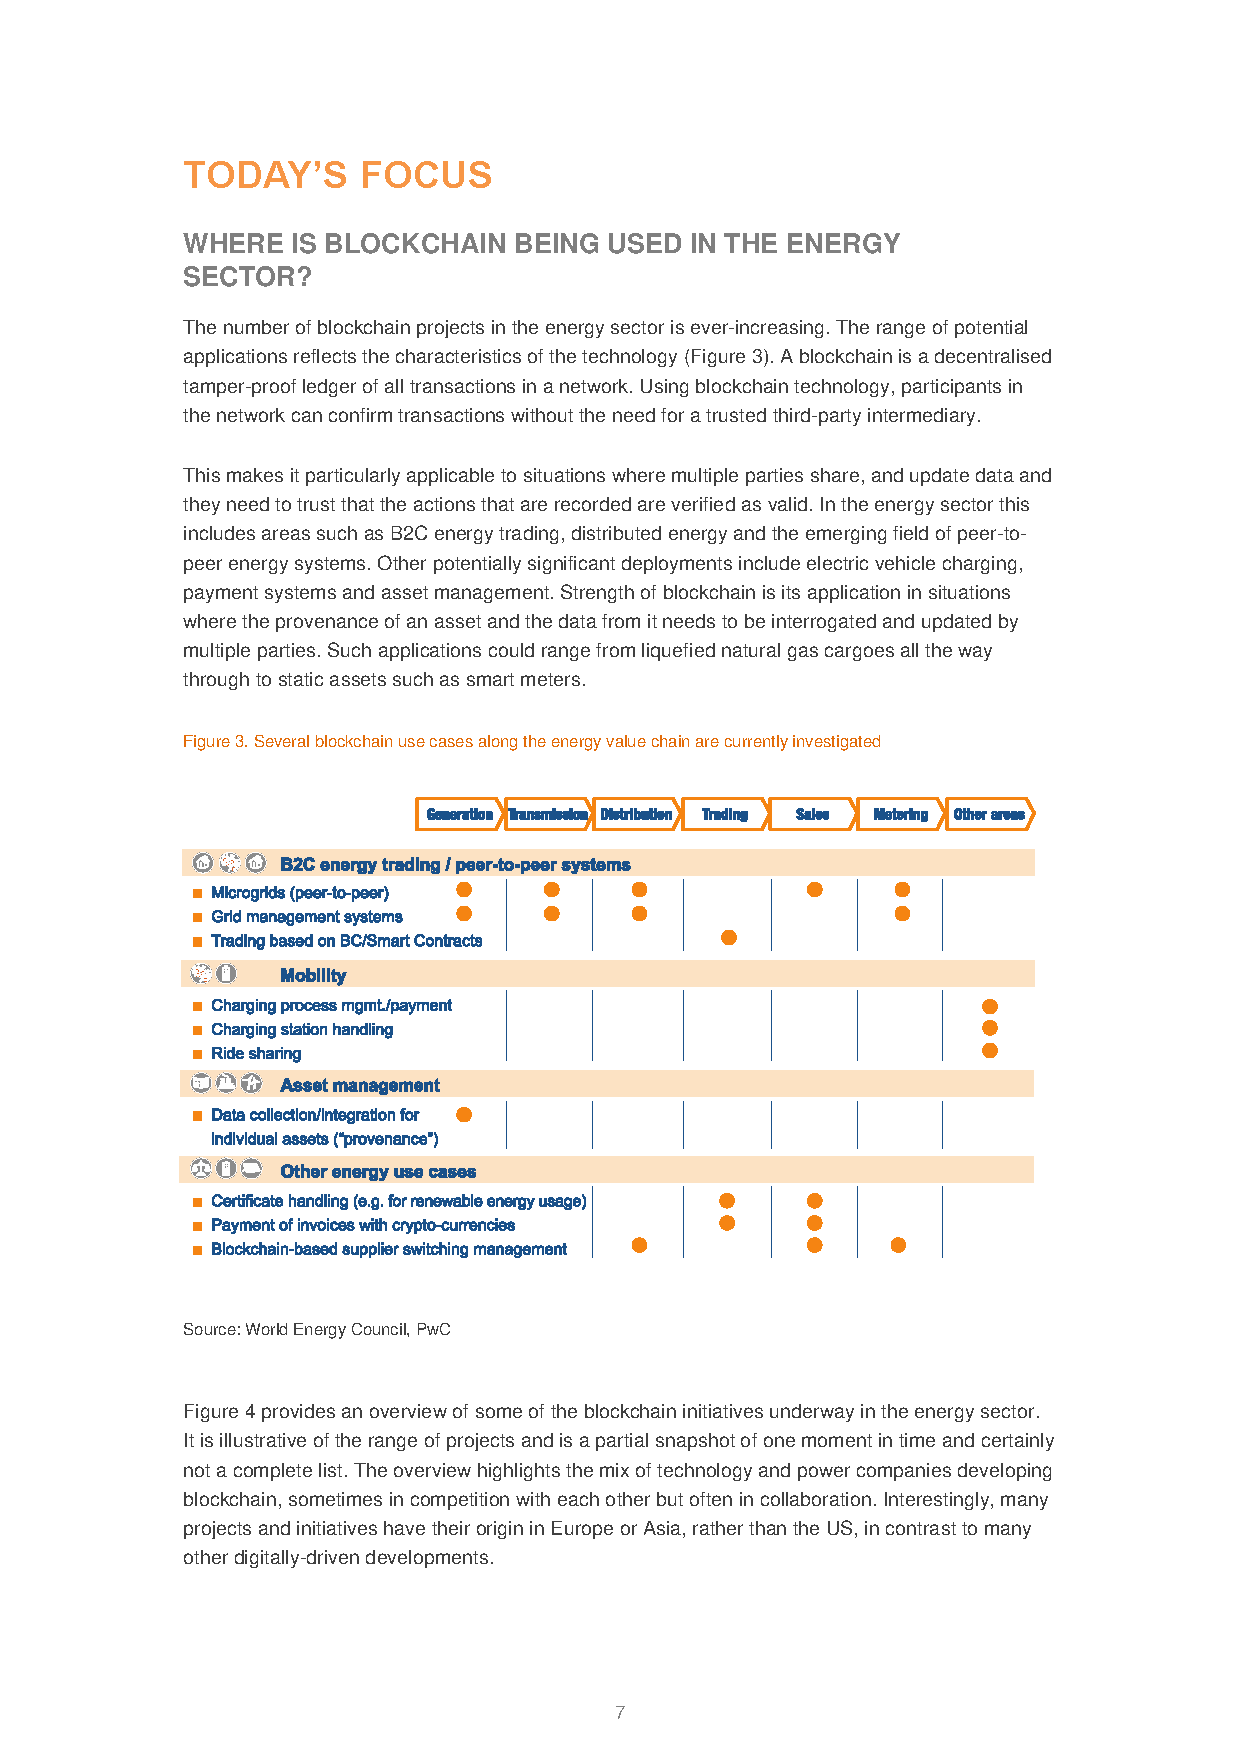
\includegraphics[clip, trim=3cm 8cm 3.25cm 13.25cm, width=\textwidth]{pics/block-on-chain.pdf}}
    \frame{\tiny
\def \bugray {\textcolor{gray}{\bullet}}
\begin{tabular}{m{2.8cm} c|c|c|c|c|c|c}
     & \multicolumn{1}{l}{\textbf{Generation}} & \multicolumn{1}{l}{\textbf{Transmission}} & \multicolumn{1}{l}{\textbf{Distribution}} & \multicolumn{1}{l}{\textbf{Trading}} & \multicolumn{1}{l}{\textbf{Sales}} & \multicolumn{1}{l}{\textbf{Metering}} & \multicolumn{1}{l}{\textbf{Other areas}} \\
 
    \multicolumn{8}{l}{\cellcolor{lightgray}B2C energy trading / peer-to-peer systems} \\
    Microgrids (peer-to-peer) & $\bugray$ & $\bugray$ & $\bugray$ \ref{brook} \textit{our proposal} & & $\bugray$ & $\bugray$ & \\
    Grid management systems & $\bugray$ & $\bugray$ & $\bugray$ & & & $\bugray$ & \ref{wien} \\
    Trading based on BC/Smart Contracts & & & \ref{pwr} & $\bugray$ \ref{alliander} \ref{ideo2} & & & \ref{wien} \\
    
    \multicolumn{8}{l}{\cellcolor{lightgray}Mobility} \\
    Charging process mgmt./payment & & & & & & & $\bugray$ \ref{rwe} \\
    Charging station handling & & & & & & & $\bugray$ \ref{rwe} \\
    Ride sharing & & & & & & & $\bugray$ \\
    
    \multicolumn{8}{l}{\cellcolor{lightgray}Asset management} \\
    Data collection/integration for individual assets ("provenance") & $\bugray$ \ref{solarcoin} & & & & & & \\
    
    \multicolumn{8}{l}{\cellcolor{lightgray}Other energy use cases} \\
    Certificate handling (e.g. for renewable energy usage) & & & & $\bugray$ & $\bugray$ & \ref{ideo1} & \ref{solshare} \\
    Payment of invoices with crypto-currencies & & & \ref{bitcoin} & $\bugray$ & $\bugray$ & & \ref{solshare} \\
    Blockchain-based supplier switching management & & & $\bugray$ & & $\bugray$ & $\bugray$ \ref{nanogrid} & \ref{ideo3} \\
\end{tabular}}
    \legend{$\bullet$ where blockchain projects are being developed.\\ $(n)$ where $n$ represents the example number presented below.}
    \source{Adapted from \citeonline{wec2017}.}
\end{table}

The electricity network use to have a top-down business model with utilities and big power generators sending electricity to customers.
Directly trade of electricity between generators and residential consumers is already a reality in the European Union (EU)~\cite{blocktrading,Brasil-futuroEE},
whilst in Brazil its mechanism is limited by the level of power consumption, and not by consumer class.

In this context,
new technologies to provide the exchange of information and to allow interactions between different autonomous agents, % agentes? conflito de nomenclatura com agentes do setor elétrico REVER!!!
embedded with artificial intelligence tools and mechanisms such as blockchain, should be a feasible solution and a trend for the next few years~\cite{Coelho2017MAS}. %[ Coelho et al., 2017].
% The presence of prosumers into the electricity market sustained by blockchain allows the share and update of data by multiple unknown parties in a trusty and verified manner~\cite{peck2017,wec2017}.
As a result, the blockchain projects can overcome the challenges with decentralized energy systems optimization,
leaving new approaches to arise, such as real-time pricing, consumers awareness about personal power consumption, prosumers awareness about when their generation is most needed, and social awareness about its impact on the grid~\cite{peck2017,wec2017}.

From this premise, worldwide solutions are being developed to enable the active participation of consumers in the electricity market as shown on \autoref{tab:block-on-energy} and described on the following \autoref{ssec:propostas}.
Therefore, for the Brazilian case, prosumers could leave a position of just accumulate energy credits to an active position, in which the excess power generated could be converted into profit. % clearing = compensação!!!

\subsection{New electricity market examples}% accordingly with \autoref{tab:block-on-energy}}
\label{ssec:propostas}

% More valuable examples (29/06/19):
% - https://innovationatwork.ieee.org/honda-gm-research-electric-vehicles-smart-grid-blockchain/
% - https://innovationatwork.ieee.org/4-blockchain-energy-companies-to-watch-in-2019/

\begin{enumerate}[label={\textcolor{gray}{(\arabic*)}}, font={\small\bfseries}]

    \item\label{solarcoin} In a more simple and international way, the \emph{SolarCoin} is a digital asset that rewards owners of solar power generation, being basically a technology to encourage decentralized, clean, and renewable energy generation,
    which aims to reduce the payback time for the solar installations~\cite{mit-dci}.
    Its crypto-currency \emph{solarcoin (SLR)} works similarly to credit cards miles program, 1 MWh is equivalent to 1 SLR.
    
    \item\label{bitcoin} On the other hand, the Marubeni company is allowing Bitcoin payments options for electricity consumption in some regions of Japan~\cite{groarke2016}.
    While a real case application in South Africa developed by Grid Singularity%
    \footnote{\href{http://gridsingularity.com}{http://gridsingularity.com}}
    uses Bitcoin transfer for accounting clearing of electricity pre-paid system \cite{video:grid}.
    
    \item\label{solshare} In Dhaka, Bangladesh, the \emph{ME SOLshare Ltd} is a social enterprise that offers \gls{p2p} trade system for solar power generation, and finance photovoltaic installations for low-income families.
    Founded in 2014, the SOLshare operates off-grid electricity in rural areas and allows its users to earn an income directly from the energy of the Sun.
    Its goal is to empower people to become entrepreneurs, enabling the creation of a bottom up smart grid, and being ready for the future integration to the power network of the country\footnote{\href{https://www.me-solshare.com/}{https://www.me-solshare.com}}.
    
    \item\label{alliander} In a similar approach, the Alliander utility aims for ``real-time'' energy trade on the Island of Texel (Holland) with smart meters linked to blockchain technology. A new business arise towards the wholesale market~\cite{groarke2016}.
    
    \item\label{nanogrid} A case of nanogrid optimization was conducted by \citeonline{magnasco2016}, in which data from a pilot nanogrid in Bangladesh was used. The authors developed a system that uses Operations Research techniques for finding the best topology of the network, defined on real-time operation with smart switches and meters.

    \item\label{brook} In the case of the \emph{Brooklyn Microgrid}, it is still limited to some consumers in Brooklyn, New York.
    The owner of a PV power can sell its generation to a neighbor using a smart contract available by the startup LO3~\cite{blocktrading}. % [Merz , 2016]
    But this model still faces regulatory issues of energy transaction, since it is under the concession area of different distribution utilities~\cite{mangelkamp2017}, which can not occur either in Brazil as stated by national \gls{gd} legislation.

    \item\label{pwr} In Australia, \emph{Power Ledger} goes a little further into the \gls{p2p} interaction, allowing the transaction between the units of a building with other consumers of the distribution grid, thanks to its tight relationship with local utility.
    Owners of a \gls{gd} can decide for who they want to sell their surplus energy and at what price.
    In the platform provided there is a mechanism of negotiation and clearing that is transparent, auditable and automated in the benefit of prosumers and consumers~\cite{pwrledger}.
    They have already expanded to Auckland area, New Zealand, with expectations that schools, community groups and residential houses participate actively in the initiative~\cite{groarke2016}.
    
    \item\label{wien} Other actions are taking place on different uses of electricity as well.
    % For instance, \emph{Fortum} enables consumers to manage theirs home consumption over internet
    % Fortum - Finland --> não achei a prov no site da empresa!
    % "Fortum aims to enable consumers to control appliances over the internet in connected homes and view blockchains as micro demand response enabler at the device level."\cite{groarke2016}
    For instance, the \emph{Wien Energie} utility uses the distributed technology to optimize and to save costs of gas trading for power generation~\cite{groarke2016}.
    Established in Austria, the system is used to guarantee the stability of the grid in case the Sun or the wind do not attend necessary demand\cite{wien-energie2016}.
    
    \item\label{rwe} And in Germany, the \emph{RWE} together with the company \emph{Slock.it}, uses the blockchain to manage electric vehicle recharge in public charging stations.
    They use an accounting unit supported by different energy suppliers in order to provide vehicle drivers a standard method of payment.
    The RWE system is based on the product \emph{BigchainDB} by Ascribe from Berlin, but it is not yet known how smart contracts are used for unlocking charging stations~\cite{blocktrading}.
    
    \item Moreover, real market applications have been tested up by the CoLab,
    an IDEO's hub for collaborative innovation, that designs human-centered projects.
    They have built three prototypes to understand blockchain potential with electricity applications.
    \begin{enumerate*}[label={\textcolor{gray}{(10.\arabic*)}}, font={\small\bfseries}]
        \item\label{ideo1} The Smart Solar
        % https://www.ideocolab.com/prototypes/smartsolar
        directly connects a solar panel to the blockchain network in order to tracks its generation, and automatically issue a personal digital Renewable Energy Certificate (REC).
        \item\label{ideo2} The Shift
        % https://www.ideocolab.com/prototypes/shift
        is a marketplace to trade energy and a self-management device to operate under power rates flexibility.
        \item\label{ideo3} And the Plug 'n' Paid
        % https://www.ideocolab.com/prototypes/plugnpaid
        is the power device manager for homes, which uses Artificial Intelligence (AI) to adjust preferences and behaviours of homeowners looking for power efficiency.
        It also manages consumption, buys power in real time, and trades power with neighboring homes accordingly with pre-charge payment.
    \end{enumerate*}
    
    % Adicionar InternetS of Energy -- DAISEE?

\end{enumerate}
%
%\chapter{The application proposal}
%\label{ch:3}
%% ch: The application proposal
% INTRO = Stakeholder Requirements Specification (StRS)

% \citeonline{mengelkamp2018} -- read
% \citeonline{mihaylov2014} -- read -- used
% \citeonline{vangulick2018} -- read
% \citeonline{kounelis2017} -- read
% \citeonline{wang2018} -- read
% \citeonline{andoni2019} -- read -- to be used

The advent of \acrfullpl{dapp} in the whole electricity chain sector has been strengthening the integration of \glspl{ict} into the power network.
Despite the technology used so far has been enough to keep the infrastructure working through third-party services,
the blockchain enables a window of wisdom at the population level, where there is a big amount of low power customers mainly fed by one source, the distribution utility.

Moreover, aware that the Brazilian \acrfull{gd} legislation is inclined to the blockchain business model,
and the expected expansion of \acrfull{der} as a consequence of consumers looking for lower tariffs and renewable power energy,
the application purpose is to allow the trade of electricity within a community that shares the responsibility of managing their own power generation for self-consumption without relying on a third-party to do so.
%Excelente paragrafo

The community scope is the group of shareable consumption, i.e., enterprises of multiple consumer units (condominiums) and shareable generation (consortiums or cooperatives).
The members of the community range from power consumers to prosumers.
Although they can't sell back their surplus generation to the power utility, they can determine the rules to transfer electricity among the group.
This measurement follows both the group self ambitions and the local legislation guidelines.
Therefore, each member has a quota from the group power generation which represents the member ownership over a given energy portion.
And it is up to the member her/himself to determine how she/he would like to distribute her/his portion.

In order to keep the group objectives of sharing the power generation and the costs to do so as a priority, without be limited by trust factors due to members nature or bad system behaviour, the proposal suggests that any modification on the current quota distribution should be made in function of a token common for the whole group.
The token represents the group digital currency and its feasibility is guaranteed by the blockchain network.
This method gets rid of mistrust, gives transparency for the whole group about any quota change, and allows a safety inspection with updated values for the utility and the legislative bodies.

Such as \gls{ico}'s initiatives, the tokens of the group have a particular method to be created.
In the present case, every time a new power plant is added into the group power capacity, a new equivalent crypto-currency amount is created.
This methodology keeps the market simple when considering the new power plants and the variety of members on each investment round.
The token issued has a low variability on the intra-market because it is proportionally created by power units, and its purpose is to exchange energy solely.
However, the cost of each power unit relies on the power plant cost to generate that energy, that depends on different weather and fund scenarios.
This makes the market unique for each member, i.e., it is up to each member's strategic vision the decision to invest in new power plants or to exchange her/his quota to get profits beyond any investment made to only cover her/his power consumption.

This kind of crypto-currency is also referred to as a non-fungible token%
\footnote{\url{https://en.wikipedia.org/wiki/Non-fungible_token}} (NFT)
because it can not be interchangeable with the blockchain native assets but works well for specific use cases.
This approach is similar to the NRGcoin~\cite{mihaylov2014} in which tokens are created by raising the power generation capacity in the distribution grid, instead of spending energy on computational power to do so.
Curiously, new power plants will emerge only when desired by members to feed their electricity needs.
So, what makes the dynamic of the internal market is the growth of members and their financial investment capacity (and interest) to fund new distributed power plants.

Therefore, there is no need to store money to exchange back the tokens to fiat currency, because each token represents individual money savings by the difference between the tariffs of the group and the utility.
Thus, the income happens similarly to the energy credit process, i.e., each member gets her/his savings after a month-round period.
And the \gls{gd} can be considered as an investment portfolio with periodic returns.
Based on those premises, the token is useful to exchange quotas without directly rely on fiat money.
%Excelente frase, tanto anterior quanto a proxima
It allows the group to determine its own valuation of the different power sources,
and it gives to each member the opportunity to speculate how much her/his quota worth at any given moment, i.e., how much she/he is inclined to accept to exchange the quota.
% A blockchain application to manage the transactions assures a reliable member-to-member deal and transparency to the group and to the power distribution utility about the updated quota values.

Finally, the proposed \gls{dapp} context can be detached into three main layers as shown by \autoref{fig:sys-lay}.
% They can be interpreted as well as the concepts presented by \autoref{fig:sys-as-is}, but with subject detailing.
The information network layer is the key part of the development because it redefines the information flux interaction that comes from both remaining layers.
So, the traditional information flux about the power grid network between consumers/prosumers and utility is unchanged, the power meter continues to register the electricity and send this information in a one-way direction.
Similarly happens to the business layer, where the fundamental practices of the group of shareable consumption keep the same, except by the information management supported by the blockchain advantages,
in what now everyone has reliable access to their counterpart members data, and a impartial communication channel to alter their quotas.

The link between both business and power networks through the information layer is the member her/himself because she/he is the only one with access to her/his electricity meter information and with write-permission to the blockchain network at the same time.
The member as a blockchain node is responsible to input the required measuring values in the information network (off-chain service) and to interact with its peers (on-chain service).

\begin{figure}[htbp]{\textwidth}
    \centering
    \frame{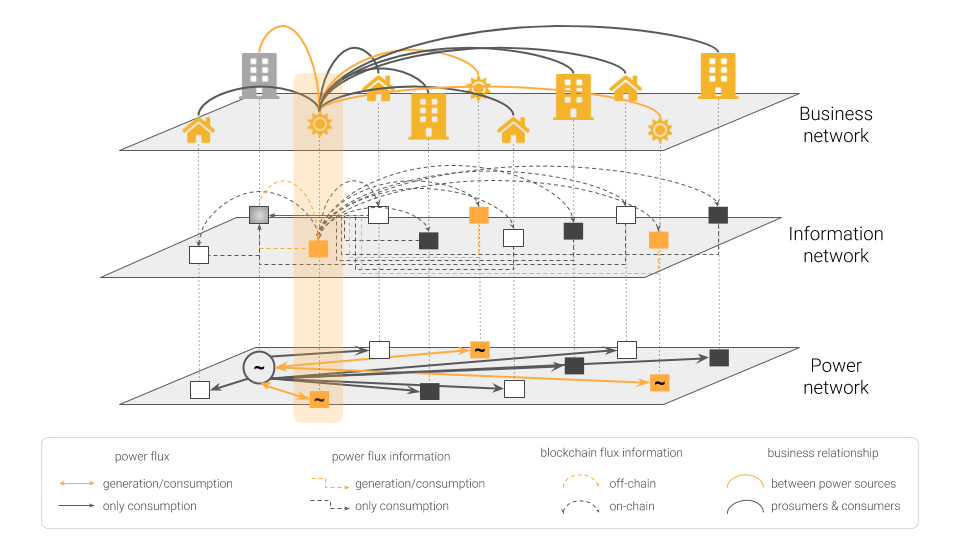
\includegraphics[width=\textwidth]{pics/dapp-op.png}} % fazer o desenho em slides primeiro e depois converter para tikz
    \caption{The operational layers of a micro/mini-grid and the blockchain approach on it from a prosumer point-of-view in a shareable generation group.}
    \label{fig:sys-lay}
    % \legend{}
    \source{Adapted from \citeonline{kounelis2017, andoni2019}.}
\end{figure}

Then, the proposed blockchain application is a small part of an entire management system to be used by the group of shareable consumption in the context of micro/mini-grid to offer to its members an intra-market to negotiate their electricity fraction earnings.
With support from the ISO/IEC/IEEE International Standard of Systems and software engineering -- Life cycle processes -- Requirements engineering (\citeyear{iso-iec-ieee}),
\autoref{sec:requisitos} describes the ordinary requirements for the \gls{dapp} developed.
The following \autoref{sec:platform} adds a comparison about some of the blockchains available on the market in order to justify the one used to develop the application.
\autoref{sec:the-dapp} presents the application itself,
and \autoref{sec:experiments} complements with a simulation about the application functionality making use of a real case of shareable consumption.

\section{Identification of the application requirements}
\label{sec:requisitos}

The design of an application requests the understanding of some system statements which captures the user needs, and associated constraints and conditions.
These requirements involve a set of specifications until reach the definitions of the software functions, performance, design constraints, and attributes~\cite{iso-iec-ieee}.
The \autoref{fig:sys-as-is} states the system approach of the whole process to develop a software, and highlight what the present work is up to advance toward a \gls{dapp}.

\def\c#1{\textbf{#1}}

\newcommand{\appschema}[4]{
\begin{figure}[h!btp]{\textwidth}
    \centering
    \caption{#1}
    {#2} % label
    
    % We need layers to draw the block diagram
    \pgfdeclarelayer{background}
    \pgfdeclarelayer{foreground}
    \pgfsetlayers{background,main,foreground}
    
    % Define a few styles and constants
    \tikzstyle{elemts}=[draw, fill=gray!20, text width=5em, text centered, minimum height=2.5em]
    \tikzstyle{target} = [draw, fill=gray!50, text width=6em, text centered, minimum height=2.5em, rounded corners]
    \tikzstyle{geral} = [rounded corners, draw=black!90]
    % \tikzstyle{ann} = [above, text width=5em]
    \tikzstyle{tbx} = [anchor=north west, text width=6em]
    % \def\blockdist{(-1,0.7)}
    \def\edgedist{(-0.2,0.2)}
    
    \def\bigtxt{\footnotesize{\c{market trends\\\medskip laws \& regulations}\\\medskip %
                legal liabilities\\\medskip social responsibilities\\\medskip \c{technology base}\\\medskip labor pool\\\medskip competing products\\\medskip \c{standards \& specifications\\\medskip public culture\\\medskip physical/natural environment}}}
    \def\bigtx{\footnotesize{policies \& procedures\\\medskip standards \& specifications\\\medskip %
                guidelines\\\medskip domain technologies\\\medskip local culture}}
    \def\bigt{\footnotesize{\c{business operational processes\\\medskip  business operational constraints}\\\medskip %
                business operational policies \& rules\\\medskip business operational modes\\\medskip business operational quality\\\medskip business structure}}
    
    \frame{%
    \resizebox{\textwidth}{!}{%
    \begin{tikzpicture}
        % general boxes
        % \node 
        \node (sftwr) [target] {Software\\(Dapp)};
        \node (sysel) [above of=sftwr] {System Element};
        \path [above of=sysel]+(0,1.5) node (elemt1) [elemts, text width=8em] {System Element};
        
        % titles
        \node (SYS) [above of=elemt1] {System};
        \path (SYS.north west)+(0,0.7) node (sysop) {System Operation};
        \path (sysop.north west)+(-2,0.7) node (bizop) {Business Operation};
        \path (bizop.north west)+(-0.5,0.7) node (orgen) {Organization Environment};
        \path (orgen.north west)+(-1.5,0.7) node (exten) {External Environment};
        
        % text boxes
        \path (bizop.south west)+(0,-0.25) node [tbx, text width=8em] {\bigt};
        \path (orgen.south west)+(0,-0.25) node [tbx] {\bigtx};
        \path (exten.south west)+(0,-0.25) node [tbx, text width=7em] {\bigtxt};
        
        % boxes of the titles
        \begin{pgfonlayer}{background}
            % External Environment
            \path (exten.north west)+\edgedist node (a) {};
            \path (sftwr.south -| sftwr.east)+(2,-1.2) node (b) {};
            \path[geral, draw=white] (a) rectangle (b);
            
            % Organization Environment
            \path (orgen.north west)+\edgedist node (a) {};
            \path (b)+(-0.2,0.2) node (b) {};
            \path[geral] (a) rectangle (b);
            
            % Business Operation
            \path (bizop.north west)+\edgedist node (a) {};
            \path (b)+(-0.2,0.2) node (b) {};
            \path[geral] (a) rectangle (b);
            
            % System Operation
            \path (sysop.north west)+\edgedist node (a) {};
            \path (b)+(-0.2,0.2) node (b) {};
            \path[rounded corners, draw=black!90, dashed] (a) rectangle (b);
            
            % System
            \path (sysel.west |- SYS.north)+(-0.4,0.2) node (a) {};
            \path (sftwr.south -| sysel.east)+(+0.4,-0.4) node (b) {};
            \path[geral] (a) rectangle (b);
            
            % System Element (of Dapp)
            % \path (sysel.north west)+(-0.2,0.2) node (a) {};
            % \path (sftwr.south -| sysel.east)+(+0.2,-0.2) node (b) {};
            % \path[elemts] (a) rectangle (b); % node 'System Element' with 'Software'
            \path let \p1=($(elemt1.west)-(elemt1.east)$), \n1 = {veclen(\p1)-\pgflinewidth},
                \p2=($(sysel.north)-(sftwr.south)$), \n2 = {veclen(\p2)} % -\pgflineheight
                in node[draw, elemts, minimum width=\n1, minimum height={1em+\n2}] at (0,0.4) (nome) {};
        \end{pgfonlayer}
    \end{tikzpicture}
    }}

    \legend{#3}
    \source{#4}
\end{figure}
}
\appschema{Concepts for the development of a system.}%
            {\label{fig:sys-as-is}}%
            {The grayer box and the bold texts highlight the propositions considered for the blockchain application development.}%
            {Adapted from \citeonline[fig.~4]{iso-iec-ieee}}

The different sets of requirement information items shown the broad range of knowledge to be considered for a fully decentralized system development.
Notwithstanding, the identification of each item requires interaction and cooperation among stakeholders, mainly to define how they interact through sets accordingly with business and system specifications.

The \autoref{fig:sys-as-is} presents the development scope from the top level environments, to the business level, to the ``specific system-of-interest''~\cite{iso-iec-ieee}.
The first addresses the external directives the system must follow, and some of the items had already been discussed (bold texts).
The second refers to the intended way of doing business, and the systems are mainly viewed as black-boxes. It is up to the group's guidelines and rules, and most of its items are out of the scope of the present work. The proposal considers only what may be universal for this business category.
At the third lays the user's viewpoint to interact with the aforementioned layers~\cite{iso-iec-ieee}.

% \section{System Requirements Specification (SyRS)}
Even not aware about all specifications, the core concept of the application can be developed with no additional issues.
In the future, the remaining features may improve the application presented here.
For instance, the definitions about how the registering of members will be conducted and how the user interface will be are out of the core of the application, i.e., the purpose to securely allow the transaction between members in a doubtful environment.

The case where the \gls{dapp} rely on off-chain platforms, such as the power meter or electricity bill of the members to gather the values from generation to input in the blockchain is another exception.
For both methods, the group guidelines must address what should be done to solve possible problems to access the information or if a violation is found.
Although a smart-contract can be held to deal with them, the subjects related to errors and penalties are out-of-bounds.

% \subsection{User requirements}
However, for sure, the application must be accessible in any device and the user experience must encompass a wide audience age.
The usability to request or to send tokens must be as easy as to send a text message,
and it may be provided by the blockchain platform chosen throughout the features available for the development.
Although it is an important aspect of the \gls{dapp} project design, the considered development is a hidden layer of the front-end project, which is not instigated.

Moreover, all the users must provide the same registration data available on their electricity bill at the first access to the blockchain environment of a particular group.
This constitutes sensitive data and it will be hidden from the public ledger.
Indeed, this process represents the step in which a user becomes a member of a group.
So, members may access those data but users not.

% \subsection{Project Constraints}
For what concerns members data, there is special attention to where members reside and if they pertain to the same power utility.
Although they could be in the same geographic area, this not implies being fed by the same distribution grid.
It is not restricted to form a group with those customers, but a transaction between them is.
Thus, each member must be classified by power utility in order to exchange tokens.

In addition, some mistakes may happen during a quota transaction,
for example one could type 100 instead of 10 when writing up her/his clause.
In other cases, get rid of the quota should be mandatory by legislation force.
As the group has a representative body to act on their behalf,
the application must allow corrective transaction to interfere on these issues accordingly to the group guidelines to do so.
It is important to remember that blockchain ledger is an append-only database, so a new transaction must be held to take its effect.
This measure doesn't compromise privacy, neither security, but guarantees a safe interference for its members.
However, to simplify, the group representation by members hierarchy was replaced by a voting process to validate the changing of any group asset.

% \paragraph{Stakeholders}
Lastly, the stakeholders involved in the system are:
\begin{enumerate*}[label={(\roman*)}]
    \item\label{con} consumers,
    \item\label{pro} prosumers,
    \item\label{pou} power utility, and
    \item\label{leg} legislator.
\end{enumerate*}
The \ref{con} and the \ref{pro} are represented by the basic role of a member of a given group.
They are the unique users of the application, and they can interchange position.
In a more common way, the former can become the latter, but the opposite is not impossible to happen.
The \ref{pou} and the \ref{leg} can read the public ledger to follow the changes in the quota, but they can't directly interact with the application.
For these ones, each member is only a hash number (the public key) which is cross-referenced on their own private database to get full identification.

For the sake of simplicity, the proposal considers that a member joins only one group, but no restriction was imposed in the code lines.
So, two members who reside in the same geographic area and who are fed by the same distribution utility may be or not part of the same group of shareable generation.

In summary, \autoref{appen:terms} gathers the terms that will be used throughout the publishing in addition to what has been presented so far.
Note that they do not represent the variables names, although they have been used to give readability for the code.
The application comprehension was designed through a \gls{uml} class diagram detailed in \autoref{appen:uml}.
There can be noticed the relationships and attributes of the \emph{reader}, the \emph{user} and the \emph{member}.
Similarly, the main concepts of the blockchain technology were detached to better identify the aforementioned application features.

% \noindent
% * How to guarantee veracity of inputed informations? \\
% ** can be changed over time by user or automatically gotten at utility system? \\
% *** The end value can be different by countability period, it will be later discussed... \\
% **** The special characteristics must be defined by cooperative rules.

\section{Choosing the right platform}
\label{sec:platform}

\subsection{Bitcoin}
\label{ssec:bitcoin}
% Bitcoin variation
    % Alguma aplicação acima?
    
% https://bitcoin.org/pt_BR/como-funciona
    
\subsection{Ethereum}
\label{ssec:ethereum}
% Ethereum
    % A maioria das aplicações apresentadas acima

\subsection{Neo}
\label{ssec:neo}
The Neo blockchain defines itself as a ``distributed network for the Smart Economy''~\cite{neowp}.
Based on the principle of digital identity, i.e., real identity information stamped in electronic form,
Neo allows a true physical asset ownership by means of a digital asset that can, in the near future, replace the Online Certificate Status Protocol (OCSP) to manage and record the X.509 Certificate Revocation List (CRL)~\cite{neowp}.
% "Our verification of identity when issuing or using digital identities includes the use of facial features, fingerprint, voice, SMS and other multi-factor authentication methods. At the same time, we will also use the blockchain to replace the Online Certificate Status Protocol (OCSP) to manage and record the X.509 Certificate Revocation List (CRL)."

The NEO blockchain digital assets has two forms of operation.
One known as global asset refers to the public system space, which involves the native assets NEO and GAS.
The other one refers to the contract assets that may follow some standards and usually have a private storage, an area created by a smart contract with restrictions to join in.
Although any new smart contract deployed on the public ledger can create its own private space, they have to follow  the NEP-5 standard (similar to Ethereum ERC-20) to keep compatibility over the whole system if they intend to create a side cryptocurrency.

Likewise most of blockchain technologies, Neo uses the native tokens to govern transactions.
The token NEO by itself represents the right to manage the network, such as voting for bookkeeping and involvement on network parameter changes.
Its value ranges from 1 to 100 million with integer steps, without subdivisions.
Its total amount was created in the genesis block and it was half divided between the supporters of NEO during the ICO and the NEO Council.
The latter manages the tokens in order to support ``NEO's long-term development, operation and maintenance and ecosystem'' and ``will not enter [into] the exchanges [processes]''~\cite{neowp}.
Therefore, who holds NEO tokens are part of the network owners and has right to manage the network by voting procedures.

The other token is the fuel to control the Neo network resources.
It is called NeoGas, abbreviated as just GAS, and has the same maximum total limit of 100 million, although its minimum unit is 0.00000001.
It is created proportionally to each NEO a peer has by a decay algorithm rate when a new block is generated.
It is used to charge transactions and smart contract operations, however some of them have no fee so far, such as those related to contract assets.
In addition, some NeoIDs have priority when a large amount of transactions happen, while others may get this benefit by paying additional GAS.

This option is valuable because the Neo consensus mechanism has a new block appending time of ... in average.
It is a quite good "waiting period" (tem um nome técnico pra isso!) compared to others \gls{dbft} blockchains, like ...
Furthermore, the distributed storage protocol utilizes the same technology used by IP management over the whole Internet, the Distributed Hash Table (DHT) technology. % VER com Igor!!
"Large files is divided into fixed-size data blocks that are distributed and stored in many different nodes."\cite{neowp}
Although this method impose a trade-off between redundancy and reliability, Neo aims to use token incentives and backbone nodes to solve it, so users may settle the requirements of a given file.
In the end, a file reliability level will be proportional to its assigned cost of store and access.

Moreover, the blockchain allows cross-chain interoperability through a protocol whose makes other smart contracts compatible with NeoContract system.
It is either possible to exchange tokens and to scatter the steps of a transaction across chains.

\textcolor{red}{Falar sobre as API's.}
 the API's to 'trackle' native and side cryptocurrencies over smart-contracts and transactions.
Since


\subsection{Tron?}
\label{ssec:tron}
% Tron

\subsection{Libra}
\label{ssec:libra}

There are many projects going on, one example is the Libra Blokchain, https://info.binance.com/en/research/marketresearch/libra.html, an alliance of JP Morgan, XXX , Facebook...

This blockchain will be used for xxx


\subsection{Hyperledger}
\label{ssec:hyperledger}

Different from the others, the Hyperledger is not a unique blockchain technology, but a family of \glspl{dlt} designed to fit diverse business requirements and allow cross-industry solutions.
It is an open source collaborative effort under the Linux Foundation with leaders in finance, banking, \gls{iot}, supply chains, manufacturing and technology~\cite{hyper1}.

Nonetheless, all the five frameworks available by the Hyperledger make use of a modular architectural design in order to ``encourage the re-use of common building blocks'', and to ``enable rapid innovation of the \gls{dlt} and the interfaces between them''~\cite{hyper2}.
Consequently it has the benefits of extensibility and flexibility,
allowing independent modification of any component in an interoperable way,
offering highly secure solutions through rich and easy-to-use \glspl{api}~\cite{hyper1, hyper2}.

Aware that business blockchain networks operates under a partial trust environment, and the requirements may represent a potentially unique optimization point for the technology~\cite{hyper2},
the resulting system design relies under the classification of permissioned blockchain network but the range between public and private definition varies by each characteristic of a specific framework.
Similarly, the whole family has a particular consensus method that not include the standard \gls{pow} with anonymous miners, neither the use of a native token nor a cryptocurrency~\cite{hyper1}.

The Hyperledger business modular approach is quite similar to what was shown at \autoref{fig:layers}.
Besides the consensus layer purpose (Layer 0), the remaining layers dive into business blockchain components of the generalized layers already presented.
For instance, the smart contract layer is part of the Layer 2a, but the provided data-stores module and identity services module can be correlated with the whole Layer 2.
Independently of where they stand -- on- or off-chain -- their purpose are to allow the better business fit by other modules.

In addition, there is a policy service module responsible for management of various system policies. It is a significant requirement to rule the application behaviour over all other modules, in this way it can be consistent with the Layer 5.
The \glspl{api} module concerns usability such as the Layer 4.
Another module is the interoperation itself (Layer 3), which supports interoperability between different blockchain instances.
The remaining modules can be correlated with the same layer.
The communication and crypto modules aims to allow ``peer-to-peer message transport between the nodes that participate in a shared ledger instance'' and ``different crypto algorithms or modules to be swapped out without affecting other modules''~\cite{hyper1}.
% mudar isso depois!

% Consensus
% FIGURE 1. GENERALIZED HYPERLEDGER CONSENSUS PROCESS FLOW --> diagrama de sequência

% "Hyperledger business blockchain frameworks reach consensus by performing two separate activities: 1. Ordering of transactions, and 2. Validating transactions"~\cite{hyper1}
% The former...
% The latter...

% When dealing with validations, it is more important to give special attention to logic errors than to syntax ones.
% For the latter, the transaction can be dropped with no significant consequences.
% But for the former, the ``errors are more complex and should be policy driven whether to continue processing or not, and we might want to log these transactions for auditing if the policy requires''~\cite{hyper1}.

Anyhow, four frameworks use a voting-based approach to consensus.
Hyperledger Fabric, Hyperledger Iroha and Hyperledger Indy by means of Apache Kafka, Sumeragi and Redundant Byzantine Fault Tolerance (RBFT), which are nothing than variations of \gls{pbft} method.
The Hyperledger Burrow uses \gls{pos} through Tendermint consensus engine\footnote{\href{https://github.com/hyperledger/burrow/}{https://github.com/hyperledger/burrow/}}.
Nonetheless, Hyperledger Sawtooth uses a lottery-based approach, the \gls{poet}~\cite{hyper1}.


% Transaction Dependencies
% "All four Hyperledger frameworks that support smart contracts assume that
% transactions are atomic.
% In other words, a transaction is considered either not yet started or else completed; a transaction cannot be partly completed.
% This ensures transaction integrity.
% When dependent actions (if this then that) must be committed together, some frameworks assume that the dependent actions are captured in a single smart contract.
% Others permit batching of transactions across multiple smart contracts.
% Thus, smart contracts can specify dependencies between multiple transactions which must be committed atomically.
% These references can be either implicit or explicit."~\cite{hyper2}

% "With an implicit reference, it is usually impossible to determine the order in which transactions must be applied.
% Bitcoin solves this by repeatedly trying to apply the transaction, which results in transactions being gradually executed as their prerequisites are satisfied.
% This behaviour requires a transaction staging component, such as mempool, which takes care of any expiring transactions the system could not apply.
% With an explicit reference, the user submitting the transactions specifies the ordering with some form of transaction identifiers.
% Just as implicit and explicit references impact the formation of the block, so does the dependency graph.
% The dependency graph can be either cyclic or acyclic, in other words, circular or non-circular.
% With cyclic dependencies, the entire group containing the cycle must be included in the same block.
% With acyclic dependencies, any portion of the sequence may be included in the block, as long as transactions are included according to the dependency graph.
% With implicit dependencies, cycles may be complex to resolve, which can prevent certain transactions from being validated in parallel and committed.
% On the other hand, explicit dependency references can allow for parallel execution of non-conflicting transactions within the same block."~\cite{hyper2}

% Smart Contracts in the Hyperledger Frameworks --> acho q tb não preciso falar sobre isso
% Fazer um resumão, pq não preciso disso tudo.
% Table 1. Smart Contract Implementations in Hyperledger Frameworks

\subsection{R3 Corda}
\label{ssec:r3corda}

% R3 Corda

% \subsection{Microsoft Azure} -- Não é uma solução da Microsoft, mas uma integração com a Hyperledger
% https://azure.microsoft.com/pt-br/solutions/blockchain/
% https://www.coindesk.com/microsoft-salesforce-join-hyperledger-enterprise-blockchain-consortium

\subsection{Comparison}

% Smart Contract Integrity and Availability
"To ensure the integrity and availability of the blockchain network and the smart contract layer, enterprise blockchains must control access to certain resources.
Since smart contracts are programs, they are vulnerable to malicious attack, coding errors, and poor design.
A breakdown in any of these areas can compromise the integrity or availability of the blockchain system."~\cite{hyper2}

"Business blockchain systems can apply time or token-based resource management techniques to ensure that any particular smart contract does not consume excessive resources."~\cite{hyper2}



% highlight features

% "However, for sure, the application must be accessible in any device and the user experience must encompasses a wide audience age.
% The usability to request or to send tokens must be as easy as send a text message,
% and it may be provided by the blockchain platform choosed."~(seção anterior)
% Quais API's estão disponíveis para facilitar isso?

% WHAT HAVE ALREADY BEEN DISCUSSED AND NEED TO BE IDENTIFIED AS FEATURES

% - technological compliance
%     - cost-effective
%     - fair
%     - robust
%     - flexibility

% - social compliance
%     - accessibility

% - blockchain application
%     - immutability
%     - non-repudiation
%     - integrity
%     - transparency
%     - equal rights

% - blockchain infrastructure
%     - scalability
%     - peer autonomy
%     - dynamic behaviour of peers (leave and join)
%     - self-organization
%     - decentralization
%     - fault-tolerance

% - permissionless OR permissioned
%     - consensus algorithm
%         - trust factor (how the consensus is met)
%         - computational power
%         - transaction speed
%     - main coin
%     - altcoin
%     - xu2017:
%         - cost efficiency
%         - performance
%         - number of failure points
%         - data/computation on/off chain

\begin{table}[h!tbp]{\textwidth}
    \centering
    \caption{To be defined...}
    \label{tab:comparison}
    \frame{% https://www.tablesgenerator.com/#

\begin{tabular}{m{2.8cm}lllllll}
                                            & \textbf{\nameref{ssec:bitcoin}} & \textbf{\nameref{ssec:ethereum}} & \textbf{\nameref{ssec:neo}} & \textbf{\nameref{ssec:tron}} & \textbf{\nameref{ssec:libra}} & \textbf{\nameref{ssec:hyperledger}} & \textbf{\nameref{ssec:r3corda}} \\
\multicolumn{8}{l}{\cellcolor[HTML]{C0C0C0}Technological Compliance}                                                                                                                                                                                                                                                                                                             \\
cost-effective                              & \multicolumn{1}{c}{}                         & \multicolumn{1}{c}{}                          & \multicolumn{1}{c}{}                     & \multicolumn{1}{c}{}                      & \multicolumn{1}{c}{}                       & \multicolumn{1}{c}{}                             & \multicolumn{1}{c}{}                         \\
fair                                        & \multicolumn{1}{c}{}                         & \multicolumn{1}{c}{}                          & \multicolumn{1}{c}{}                     & \multicolumn{1}{c}{}                      & \multicolumn{1}{c}{}                       & \multicolumn{1}{c}{}                             & \multicolumn{1}{c}{}                         \\
robust                                      & \multicolumn{1}{c}{}                         & \multicolumn{1}{c}{}                          & \multicolumn{1}{c}{}                     & \multicolumn{1}{c}{}                      & \multicolumn{1}{c}{}                       & \multicolumn{1}{c}{}                             & \multicolumn{1}{c}{}                         \\
flexibility                                 &                                              &                                               &                                          &                                           &                                            &                                                  &                                              \\
\multicolumn{8}{l}{\cellcolor[HTML]{C0C0C0}Social Compliance}                                                                                                                                                                                                                                                                                                                    \\
accessibility                               & \multicolumn{1}{c}{}                         & \multicolumn{1}{c}{}                          & \multicolumn{1}{c}{}                     & \multicolumn{1}{c}{}                      & \multicolumn{1}{c}{}                       & \multicolumn{1}{c}{}                             & \multicolumn{1}{c}{}                         \\
\multicolumn{8}{l}{\cellcolor[HTML]{C0C0C0}Blockchain Application}                                                                                                                                                                                                                                                                                                               \\
imutability                                 & \multicolumn{1}{c}{}                         & \multicolumn{1}{c}{}                          & \multicolumn{1}{c}{}                     & \multicolumn{1}{c}{}                      & \multicolumn{1}{c}{}                       & \multicolumn{1}{c}{}                             & \multicolumn{1}{c}{}                         \\
non-repudiation                             &                                              &                                               &                                          &                                           &                                            &                                                  &                                              \\
integrity                                   &                                              &                                               &                                          &                                           &                                            &                                                  &                                              \\
transparency                                &                                              &                                               &                                          &                                           &                                            &                                                  &                                              \\
equal rights                                &                                              &                                               &                                          &                                           &                                            &                                                  &                                              \\
\multicolumn{8}{l}{\cellcolor[HTML]{C0C0C0}Blockchain Infrastructure}                                                                                                                                                                                                                                                                                                            \\
scalability                                 & \multicolumn{1}{c}{}                         & \multicolumn{1}{c}{}                          & \multicolumn{1}{c}{}                     & \multicolumn{1}{c}{}                      & \multicolumn{1}{c}{}                       & \multicolumn{1}{c}{}                             & \multicolumn{1}{c}{}                         \\
peer autonomy                               & \multicolumn{1}{c}{}                         & \multicolumn{1}{c}{}                          & \multicolumn{1}{c}{}                     & \multicolumn{1}{c}{}                      & \multicolumn{1}{c}{}                       & \multicolumn{1}{c}{}                             & \multicolumn{1}{c}{}                         \\
dynamic behaviour of peers (leave and join) & \multicolumn{1}{c}{}                         & \multicolumn{1}{c}{}                          & \multicolumn{1}{c}{}                     & \multicolumn{1}{c}{}                      & \multicolumn{1}{c}{}                       & \multicolumn{1}{c}{}                             & \multicolumn{1}{c}{}                         \\
self-organization                           &                                              &                                               &                                          &                                           &                                            &                                                  &                                              \\
decentralization                            &                                              &                                               &                                          &                                           &                                            &                                                  &                                              \\
fault-tolerance                             &                                              &                                               &                                          &                                           &                                            &                                                  &                                              \\
\multicolumn{8}{l}{\cellcolor[HTML]{C0C0C0}Permissionless or Permissioned}                                                                                                                                                                                                                                                                                                       \\
consensus algorithm                         &                                              &                                               &                                          &                                           &                                            &                                                  &                                              \\
main coin                                   &                                              &                                               &                                          &                                           &                                            &                                                  &                                              \\
altcoin                                     &                                              &                                               &                                          &                                           &                                            &                                                  &                                              \\
\textit{cost efficiency}                    &                                              &                                               &                                          &                                           &                                            &                                                  &                                              \\
\textit{performance}                        &                                              &                                               &                                          &                                           &                                            &                                                  &                                              \\
\textit{number of failure points}           &                                              &                                               &                                          &                                           &                                            &                                                  &                                              \\
\textit{data/computation on/off chain}      &                                              &                                               &                                          &                                           &                                            &                                                  &                                             
\end{tabular}}
    % \legend{}
    % \source{}
\end{table}

\section{The Dapp specifications}
\label{sec:the-dapp}
% \section{The Dapp requirements specification}
% \section{The distributed application}
% \section{Software Requirements Specification (SRS)}

% "Ongoing discussions revolve around the following questions:
% - Who should own and operate a distribution-level market?
% - What should the market rules and product definitions look like?
% - How should wholesale- and retail-level energy markets interact?"
% - What are the costs and benefits of TE, really?"~\cite{masiello2016}

% "This article ~\cite{masiello2016} provides a good summary of the market and technology issues to be faced down each of two paths for implementation—should there be a hierarchy of wholesale-level independent service operators (ISOs) and retail-level DSOs or one big centralized market/system operator?"

The \gls{dapp} purpose is to allow members from a group of shareable consumption to safely interact to exchange their power assets and to give transparency to others about their transactions.
For this end, the application is composed by one smart contract responsible to define the group-centered blockchain environment apart of the main blockchain network.
This is important to protect members' data from public access and to guarantee the transactions only between them.

The developed smart contract, also called as \gls{mtemsm}, has several functions and restrictions to deal with different kinds of transaction.
Its has its own public address after being deployed on the main blockchain network.
From the system interface, any user can make a transaction with this smart contract address to invoke a specific function.
Note that it is not required to transfer \emph{NEO coins}, but a transaction fee in \emph{GAS} exist and must be payed by whoever request the transaction.
By the same interface, anyone can track the transactions results based on the publishing \emph{events} or any other return argument, from (dis)approval to join the group, to modifications on a member's dataset.

Although those types of information in the blockchain ledger can be accessible by everyone, some of them are restricted by user levels.
Thereby, any cryptographic result remains for public access while some general information about the group can be accessed through any user account, and the cross-referencing between real-world identification with the blockchain digital identity keeps accessible only to members.
\Autoref{fig:flow-mtemsm} presents an overview of the \gls{mtemsm} interface with three sets of operations, namely:
\begin{description} % emph
    \item[General] provides only one function for users to request to join the group.
    
    \item[Partially restricted] also provides only one function but with restrictions based on what information is requested. So members and users have different access by each statement provided, which can be about the group power capacity, the group number of members, a given power plant registration data, or a member dataset.
    
    \item[Restricted] provides the main functions for members to vote on a process, to bid on a power plant crowdfunding, or to transact between them. Moreover, some administrative functions are also available to handle off-chain operations. Neither of these functions is restricted by members hierarchy but any other user interaction will not be allowed.
\end{description}

\begin{figure}[h!tbp]{\textwidth}
    \centering
    \caption{Available functions organized by operations access over a transaction with the \gls{mtemsm}.}
    \label{fig:flow-mtemsm}
    \frame{\resizebox{\textwidth}{!}{\begin{tikzpicture}

    % Specification of nodes
    \node (s1)  []                                  {EVENTS};
    \node (s2)  [right=of s1]                       {GLOBAL VARIABLES};
    \node (s3)  [below=of s1.west, anchor=west]     {THE MAIN INTERFACE};
    
    \node (o1)    [onchain, below=of s3.west, anchor=west]  {General operation.};
    \node (o2)    [onchain, right=of o1]                    {Partially restricted operation.};
    \node (o3)    [onchain, right=of o2]                    {Restricted operations.};
    \node (o4)    [onchain, below=of o3, xshift=1.5cm]      {Group operations.};
    \node (o5)    [onchain, below=of o4]                    {Administrative operations.};
    
    \node (s4)  [below=of o1.west, anchor=west, yshift=-5cm]    {GROUP FUNCTIONS};
    \node (s5)  [right=of s4]                                   {SYSTEM FUNCTIONS};
    \node (s6)  [right=of s5]                                   {ADMINISTRATIVE FUNCTIONS};
    
    \node (s7)  [below=of s4.west, anchor=west]     {METHODS FOR MEMBERS};
    \node (s8)  [right=of s7]                       {METHODS FOR POWER PLANTS};
    \node (s9)  [right=of s8]                       {METHODS FOR REFERENDUMS};
    \node (s10) [below=of s9.east, anchor=east]     {METHODS TO FINANCE A NEW POWER PLANT (aka an ICO of a NFT)};
    
    % Identification of the system interface
    \draw (s3.north west) rectangle (o5.south east);
    
    % Identification of the system integration
    \draw[thick, dashed] (s1.north west) rectangle (s2.south east);
    \draw[thick, dashed] (s4.north west) rectangle (s6.south east);
    \draw[thick, dashed] (s7.north west) rectangle (s10.south east);
    
\end{tikzpicture}}}
    \source{\copyright}
\end{figure}

As initially observed, the \gls{dapp} does not cover all aspects to the management system but its core agents, objects and relationships are detailed in the UML diagram on \Autoref{appen:uml}.
This representation supports the development of the following functions related to the operations described above.
In addition, it is possible to get a broad view of the \gls{mtemsm} integration with the main blockchain network, its services, and off-chain interface.
It also has a member-centered approach to better handle with the system management purpose.

Moreover, three other specifications were considered throughout the \gls{dapp} development.
One concerns to financial subjects. So a lot of decisions are carefully taken before reach the final desired result in order to shrink the amount of GAS consumed.
This methodology is based on the suggestions provided by a post on \emph{Medium}%
\footnote{\href{https://medium.com/@gongxiaojing0825/practical-tips-in-developing-neo-smart-contract-a872a4f910c1}{Practical Tips in Developing NEO Smart Contracts}},
and on the computing expenses table at NEO blockchain system%
\footnote{\href{https://docs.neo.org/docs/en-us/sc/fees.html}{NEO System Fees}}.

The other concerns to the NeoVM limitations to compile the full C# library.
For instance, most of C# integral types are converted to \verb|BigInteger| type in the NeoVM.
So, initially, the \gls{mtemsm} was designed with only the variables types allowed by the compiler.
However, the cost to storage a \verb|byte| (\verb|unit8|) variable is ..., even been converted to \verb|BigInteger|.
While a ``native'' \verb|BigInteger| variable will always cost ...
This way, a more detailed definition of the variables types were considered to better handle with an economic development.
And it has also supported a better description of the code.

The last specification is the time stamp format used, a important variable to deal on a distributed environment.
NEO system uses Unix time stamp to synchronize its operations.
It represents the date and hour running time in seconds since January 1st, 1970 at UTC%
\footnote{\href{https://en.wikipedia.org/wiki/Unix_time}{Unix time}}.
Therefore, all constants and variables of time were defined in this format.
Even the time frames considered are multiple of seconds, for instance a 30 days period has a constant value of 259200 seconds.
And none time conversion was implemented to deal with input variables different from this format because it must be handled off-chain.

At a glance, each of the developed functions behaviours are described in the following subsections.
The pseudo-codes catch all cases when faced with any kind of input, from how it is processed, to how the output is generated.



%------------------------------------------------------
% 10. External interfaces - Define all inputs into and outputs from the software system. The description should complement the interface descriptions in 9.5.3.3.1 through 9.5.3.3.5, and should not repeat information there.
% Each interface defined should include the following content:
% Jmen caliss para os inputs!
% COLOCAR NOS \paragraph{}
% Necessário detalhar como são as notificações, publicações de eventos e registros na blockchain!

% 11. Functions - Define the fundamental actions that have to take place in the software in accepting and processing the inputs and in processing and generating the outputs, including
% COLOCAR NOS \paragraph{}

\subsection*{Function \texttt{admission}}

It is the entry way to the group environment to share the benefit and cost of a \gls{gd}.

Any user can make a transaction with the \gls{mtemsm} address through the function \verb|Admission| to request to join the group.
...

To take part of it, a NEO user must request access to the group environment through a transaction with the related smart contract address.
After the approval, the user is identified inside the group and can make use of other functions and smart contracts belonging to this private environment.
\autoref{fig:flow-mtemsm} shows this workflow and at \autoref{appen:2} is the related smart contract code.

Furthermore, after an approval, the \gls{mtemsm} stores the member personal data on the internal smart contract memory space, and hence, the member could access other functions to interact with other members.

\hline

\gls{mem} is the class which managers each member registering data, both personal and ``economic'' ones.
It has the functions to check the individual balance of tokens and the shares of the group's power.
It also has an option to get the most updated values from a member or from the whole group all at once.

\begin{figure}[h!tbp]{\textwidth}
    \centering
    \caption{A user point-of-view process to be accepted in a group's private environment.}
    \label{fig:flow-admision}
    \frame{\resizebox{\textwidth}{!}{\begin{tikzpicture}

    % Specification of nodes
    \node (start) [terminal]                    {Activity starts.};
    
    \node (d1)    [decision, below=of start]    {Were all the required inputs provided?};
    \node (d2)    [decision, below=of d1]       {Does the address provided belong to the invoker?};
    \node (d3)    [decision, below=of d2]       {Is the invoker already a member?};
    
    \node (e1)    [i-o, right=of d2]            {Displays an error message.};
    
    \node (o1)    [onchain, below=of d3]        {Gets the inputs provided.};
    \node (o2)    [onchain, below=of o1]        {Creates and stores an ID for follow-up.};
    
    \node (e2)    [i-o, right=of o2]            {Displays the request from the invoker.};
    \node (e3)    [i-o, right=of e2]            {Returns the ID.};
    
    \node (o3)    [offchain, right=of e3]       {Waits a time frame period to keep going.};
    \node (o4)    [onchain, below=of o3]        {During a time frame, members can vote on this ID.};
    \node (o5)    [onchain, right=of o3]        {Any member resumes the process.};
    
    \node (d4)    [decision, above=of o5]       {Was the ID provided?};
    \node (d5)    [decision, above=of d4]       {Did the time frame pass out?};
    
    \node (o6)    [onchain, right=of d5]        {Calculates the result.};
    
    \node (d6)    [decision, above=of o6]       {Is the membership request approved?};
    
    \node (o7)    [onchain, right=of d6]        {Stores the new member dataset.};
    
    \node (e4)    [i-o, above=of d6]            {Displays the disapproval.};
    \node (e5)    [i-o, right=of e4]            {Displays the approval.};
    
    \node (end)   [terminal, above=of e4]       {Activity ends.};


    % Specification of lines between nodes defined above with additional nodes for description.
    \draw[->]  (start) -- (d1);
    \draw[->]     (o1) -- (o2);
    \draw[->]     (o2) -- (e2);
    \draw[->]     (e2) -- (e3);
    \draw[->]     (e3) -- (o3);
    \draw[->]     (e3) |- (o4);
    \draw[->]     (o3) -- (o5);
    \draw[->]     (o5) -- (d4);
    \draw[->]     (o6) -- (d6);
    \draw[->]     (o7) -- (e5);
    \draw[->]     (e4) -- (end);
    \draw[->]     (e5) |- (end);

    \draw[->]     (d1) -- node[left=2.5mm]  {Yes} (d2);
    \draw[->]     (d2) -- node[left=2.5mm]  {Yes} (d3);
    \draw[->]     (d4) -- node[left=2.5mm]  {Yes} (d5);
    \draw[->]     (d5) -- node[above=2.5mm] {Yes} (o6);
    \draw[->]     (d6) -- node[above=2.5mm] {Yes} (o7);
    \draw[->]     (d3) -- node[left=2.5mm]  {No}  (o1);
    \draw[->]     (d2) -- node[above=2.5mm] {No}  (e1);
    \draw[->]     (d6) -- node[left=2.5mm]  {No}  (e4);
    \draw[->]     (d1) -| node[pos=0.25, above=2.5mm] {No}  (e1);
    \draw[->]     (d3) -| node[pos=0.25, above=2.5mm] {Yes} (e1);
    \draw[->]     (d4) -| node[pos=0.25, above=2.5mm] {No}  (e1);
    \draw[->]     (d5) -| node[pos=0.25, above=2.5mm] {No}  (e1);
    
    \draw[->]     (e1) -- ++(4cm,0) |- (end) node {};
    
\end{tikzpicture}}}
    \source{\copyright}
\end{figure}

\subsection*{Function \texttt{summary}}

\begin{figure}[h!tbp]{\textwidth}
    \centering
    \caption{The process to get information from the group.}
    \frame{\resizebox{0.5\textwidth}{!}{\begin{tikzpicture}

    % Specification of nodes
    \node (start) [terminal]                    {Activity starts.};
    
    \node (d1)    [decision, below=of start]    {Were all the required inputs provided?};
    \node (d2)    [decision, below=of d1]       {Is the invoker not a member and the ID argument an address?};
    
    \node (e1)    [i-o, right=of d1]            {Displays an error message.};
    
    \node (o1)    [onchain, below=of d2]        {Gets the inputs provided.};
    
    \node (d3)          [decision, below=of o1]       {Is the \emph{key} a member address?};
        \node (d4)      [decision, right=of d3]       {Is the optional argument empty?};
            \node (e2)  [i-o, right=of d4]            {Returns a member's dataset information.};
        \node (d5)      [decision, below=of d4]       {Is the optional argument equal to \verb|"detailed"|?};
            \node (e3)  [i2o, right=of d5]            {Returns a member's dataset information and all PP IDs she/he has a quota on.};
        \node (o2)      [onchain, below=of d5]        {The optional argument is equal to something else.};
        \node (e4)      [i-o, right=of o2]            {Returns the respective information stored.};
    
    
    \node (d6)      [decision, left=of d3]       {Is the \emph{key} a PP ID?};
        \node (d7)  [decision, left=of d6]       {Is the PP operational?};
            
            % Yes, PP is operational.
            \node (d8)      [decision, left=of d7]      {Is the optional argument empty?};
                \node (e5)  [i-o, left=of d8]           {Returns a PP's dataset information.};
            \node (d9)      [decision, below=of d8]     {Is the optional argument equal to \verb|"detailed"|?};
                \node (e6)  [i2o, left=of d9]           {Returns a PP's dataset information and all member addresses it has shares with.};
            \node (o3)      [onchain, below=of d9]      {The optional argument is equal to something else.};
            \node (e7)      [i-o, left=of o3]           {Returns the respective information stored.};
        
            % No, PP is not operational.
            \node (d10)     [decision, below=of d7, yshift=-10cm] {Is the optional argument empty?};
                \node (e8)  [i-o, left=of d10]                    {Returns a PP's crowdfunding information.};
            \node (d11)     [decision, below=of d10]              {Is the optional argument equal to \verb|"detailed"|?};
                \node (e9)  [i2o, left=of d11]                    {Returns a PP's crowdfunding information and all member addresses whose have bided on it if it has succeed.};
            \node (o4)      [onchain, below=of d11]               {The optional argument is equal to something else.};
            \node (e10)     [i-o, left=of o4]                     {Returns the respective information stored.};
    
    \node (d12)         [decision, below=of d3, yshift=-10cm]       {Is the \emph{key} a referendum ID?};
        \node (d13)     [decision, right=of d12]                    {Is the optional argument empty?};
            \node (e11) [i-o, right=of d13]                         {Returns a referendum's process information.};
        \node (o5)      [onchain, below=of d13]                     {The optional argument is equal to something else.};
        \node (e12)     [i-o, right=of o5]                          {Returns the respective information stored.};
    
    \node (o6)      [onchain, below=of d12, yshift=-5cm]        {The \emph{key} is equal to something else.};
    \node (e13)     [i-o, right=of o6]                          {Returns a summary of the group.};
    
    \node (end)   [terminal, below=of e13, yshift=-4cm]       {Activity ends.};
    
    \node[right=of end, xshift=8cm] (ref1) {};
    \node[left=of end, xshift=-28cm] (ref2) {};

    % Specification of lines between nodes defined above with additional nodes for description.
    \draw[->] (start) -- (d1);
    \draw[->]    (o1) -- (d3);
    \draw[->]    (o2) -- (e4);
    \draw[->]    (o3) -- (e7);
    \draw[->]    (o4) -- (e10);
    \draw[->]    (o5) -- (e12);
    \draw[->]    (o6) -- (e13);

    \draw[->]     (d1) -- node[left=2.5mm]  {Yes} (d2);
    \draw[->]     (d2) -- node[left=2.5mm]  {Yes} (o1);
    \draw[->]     (d3) -- node[above=2.5mm] {Yes} (d4);
    \draw[->]     (d4) -- node[above=2.5mm] {Yes} (e2);
    \draw[->]     (d5) -- node[above=2.5mm] {Yes} (e3);
    \draw[->]     (d6) -- node[above=2.5mm] {Yes} (d7);
    \draw[->]     (d7) -- node[above=2.5mm] {Yes} (d8);
    \draw[->]     (d8) -- node[above=2.5mm] {Yes} (e5);
    \draw[->]     (d9) -- node[above=2.5mm] {Yes} (e6);
    \draw[->]    (d10) -- node[above=2.5mm] {Yes} (e8);
    \draw[->]    (d11) -- node[above=2.5mm] {Yes} (e9);
    \draw[->]    (d12) -- node[above=2.5mm] {Yes} (d13);
    \draw[->]    (d13) -- node[above=2.5mm] {Yes} (e11);

    \draw[->]     (d1) -- node[above=2.5mm] {No}  (e1);
    \draw[->]     (d3) -- node[above=2.5mm] {No}  (d6);
    \draw[->]     (d4) -- node[left=2.5mm]  {No}  (d5);
    \draw[->]     (d5) -- node[left=2.5mm]  {No}  (o2);
    \draw[->]     (d7) -- node[left=2.5mm]  {No}  (d10);
    \draw[->]     (d8) -- node[left=2.5mm]  {No}  (d9);
    \draw[->]     (d9) -- node[left=2.5mm]  {No}  (o3);
    \draw[->]    (d10) -- node[left=2.5mm]  {No}  (d11);
    \draw[->]    (d11) -- node[left=2.5mm]  {No}  (o4);
    \draw[->]    (d12) -- node[left=2.5mm]  {No}  (o6);
    \draw[->]    (d13) -- node[left=2.5mm]  {No}  (o5);
    
    \draw[->]     (d2) -| node[pos=0.25, above=2.5mm] {No}  (e1);
    \draw[->]     (d6) |- node[pos=0.25, left=2.5mm]  {No}  (d12);
    
    \draw[->]    (e1) -| (ref1) -- (end);
    \draw[->]    (e2) -| (ref1) -- (end);
    \draw[->]    (e3) -| (ref1) -- (end) ;
    \draw[->]    (e4) -| (ref1) -- (end) ;
    \draw[->]    (e5) -| (ref2) -- (end);
    \draw[->]    (e6) -| (ref2) -- (end);
    \draw[->]    (e7) -| (ref2) -- (end) ;
    \draw[->]    (e8) -| (ref2) -- (end) ;
    \draw[->]    (e9) -| (ref2) -- (end) ;
    \draw[->]   (e11) -| (ref1) -- (end);
    \draw[->]   (e10) |- (end) ;
    \draw[->]   (e12) |- (end) ;
    \draw[->]   (e13) -- (end);
    
\end{tikzpicture}}}
    % \legend{}
    \source{\copyright}
\end{figure}

\subsection*{Function \texttt{bid}}

\begin{figure}[h!tbp]{\textwidth}
    \centering
    \caption{A general bid procedure during a new power plant crowdfunding process.}
    \frame{\resizebox{0.5\textwidth}{!}{\begin{tikzpicture}

    % Specification of nodes
    \node (start) [terminal]                    {Activity starts.};
    
    \node (d1)    [decision, below=of start]    {Were all the required inputs provided?};
    \node (d2)    [decision, below=of d1]       {Does the address provided belong to the invoker?};
    \node (d3)    [decision, below=of d2]       {Is the provided PP ID a valid one?};
    \node (d4)    [decision, below=of d3]       {Does the invoker belong to the same power utility as the PP under funding?};
    \node (d5)    [decision, below=of d4]       {Is it offered a factual value?};
    \node (d6)    [decision, below=of d5]       {Still time to bid?};
    
    \node (e1)    [i-o, right=of d3]            {Displays an error message.};
    
    \node (o1)    [onchain, below=of d6]        {Gets the inputs provided.};
    
    \node (d7)    [decision, right=of o1, xshift=2.4mm]       {Is the bid value greater than the remaining deal?};
    
    \node (o2)    [onchain, right=of d7]        {Increases the value gathered so far.};
    \node (o3)    [onchain, above=of o2]        {Increases the number of contributions.};
    \node (o4)    [onchain, above=of o3]        {Keeps an identified record of the bid.};
    
    \node (e2)    [i-o, above=of o4]            {Displays the bid statement.};
    \node (e3)    [i-o, above=of e2]            {Returns \verb|"true"|.};
    
    \node (end)   [terminal, above=of e3]       {Activity ends.};


    % Specification of lines between nodes defined above with additional nodes for description.
    \draw[->]  (start) -- (d1);
    \draw[->]     (o1) -- (d7);
    \draw[->]     (o2) -- (o3);
    \draw[->]     (o3) -- (o4);
    \draw[->]     (o4) -- (e2);
    \draw[->]     (e2) -- (e3);
    \draw[->]     (e1) -| (end);
    \draw[->]     (e3) -- (end);

    \draw[->]     (d1) -- node[left=2.5mm]  {Yes} (d2);
    \draw[->]     (d2) -- node[left=2.5mm]  {Yes} (d3);
    \draw[->]     (d3) -- node[left=2.5mm]  {Yes} (d4);
    \draw[->]     (d4) -- node[left=2.5mm]  {Yes} (d5);
    \draw[->]     (d5) -- node[left=2.5mm]  {Yes} (d6);
    \draw[->]     (d6) -- node[left=2.5mm]  {Yes} (o1);
    \draw[->]     (d7) -- node[pos=0.03, left=2.5mm]  {Yes} (e1);
    
    \draw[->]     (d3) -- node[above=2.5mm] {No}  (e1);
    
    \draw[->]     (d1) -| node[pos=0.25, above=2.5mm] {No}  (e1);
    \draw[->]     (d2) -| node[pos=0.25, above=2.5mm] {No}  (e1);
    \draw[->]     (d4) -| node[pos=0.25, above=2.5mm] {No}  (e1);
    \draw[->]     (d5) -| node[pos=0.25, above=2.5mm] {No}  (e1);
    \draw[->]     (d6) -| node[pos=0.25, above=2.5mm] {No}  (e1);
    \draw[->]     (d7) -- node[pos=0.25, above=2.5mm] {No}  (o2);
    
\end{tikzpicture}}}
    % \legend{}
    \source{\copyright}
\end{figure}

\subsection*{Function \texttt{vote}}

\acrfull{vfm}

\begin{figure}[h!tbp]{\textwidth}
    \centering
    \caption{A general voting procedure called by a member.}
    \frame{\resizebox{0.5\textwidth}{!}{\begin{tikzpicture}

    % Specification of nodes
    \node (start) [terminal]                    {Activity starts.};
    
    \node (d1)    [decision, below=of start]    {Were all the required inputs provided?};
    \node (d2)    [decision, below=of d1]       {Does the address provided belong to the invoker?};
    \node (d3)    [decision, below=of d2]       {Still time to vote?};
    
    \node (e1)    [i-o, right=of d2]            {Displays an error message.};
    
    \node (o1)    [onchain, below=of d3]        {Gets the inputs provided.};
    \node (o2)    [onchain, below=of o1]        {Increases the number of votes on the respective process.};
    
    \node (d4)    [decision, right=of o2]       {Is the vote in favor?};
    
    \node (o3)    [onchain, right=of d4, xshift=1cm]        {Increases the number of \verb|"trues"|.};
    
    \node (e2)    [i-o, above=of o3]            {Displays the vote statement.};
    \node (e3)    [i-o, above=of e2]            {Returns the vote answer.};
    
    \node (end)   [terminal, above=of e3]       {Activity ends.};


    % Specification of lines between nodes defined above with additional nodes for description.
    \draw[->]  (start) -- (d1);
    \draw[->]     (o1) -- (o2);
    \draw[->]     (o2) -- (d4);
    \draw[->]     (e2) -- (e3);
    \draw[->]     (o3) -- (e2);
    \draw[->]     (e1) -| (end);
    \draw[->]     (e3) -- (end);

    \draw[->]     (d1) -- node[left=2.5mm]  {Yes} (d2);
    \draw[->]     (d2) -- node[left=2.5mm]  {Yes} (d3);
    \draw[->]     (d3) -- node[left=2.5mm]  {Yes}  (o1);
    \draw[->]     (d4) -- node[above=2.5mm] {Yes} (o3);
    
    \draw[->]     (d2) -- node[above=2.5mm] {No}  (e1);
    \draw[->]     (d1) -| node[pos=0.25, above=2.5mm] {No}  (e1);
    \draw[->]     (d3) -| node[pos=0.25, above=2.5mm] {No} (e1);
    \draw[->]     (d4) |- node[pos=0.25, left=2.5mm]  {No}  (e2);
    
\end{tikzpicture}}}
    % \legend{}
    \source{\copyright}
\end{figure}

\subsection*{Function \texttt{trade}}

\acrfullpl{tesm}

% Description of a trade process
A member can send/receive tokens from anyone else with a cost agreed upon themselves (an off-chain communication process).
It restricts null values of quotas, but not null cost values, which can be interpreted as a donation.
The \gls{mem} posts an event every time it is triggered in order to keep the group transparency about the quota shares.

\begin{figure}[h!tbp]{\textwidth}
    \centering
    \caption{A transactive energy process between members.}
    \frame{\resizebox{0.5\textwidth}{!}{\begin{tikzpicture}

    % Specification of nodes
    \node (start) [terminal]                    {Activity starts.};
    
    \node (d1)    [decision, below=of start]    {Were all the required inputs provided?};
    \node (d2)    [decision, below=of d1]       {Does the first address provided belong to the invoker?};
    \node (d3)    [decision, below=of d2]       {Is the exchange address a valid one?};
    \node (d4)    [decision, below=of d3]       {Is the exchange address also a member?};
    \node (d5)    [decision, below=of d4]       {Do both addresses belong to the same power utility?};
    \node (d6)    [decision, below=of d5]       {Are there provided factual values for trade?};
    
    \node (e1)    [i-o, right=of d3]            {Displays an error message.};
    
    \node (o1)    [onchain, below=of d6]        {Gets the inputs provided.};
    \node (o2)    [onchain, right=of o1]        {Gets the assets (quota and tokens) from each address.};
    
    \node (d7)    [decision, right=of o2]       {Do both addresses have enough assets to be exchanged?};
    
    \node (e2)    [i-o, above=of d7]            {Returns \verb|"false"|.};
    
    \node (o3)    [onchain, right=of d7]        {Decreases the quota from the first address by the exchange portion.};
    \node (o4)    [onchain, right=of o3]        {Increases the quota of the second address with the exchange portion.};
    \node (o5)    [onchain, above=of o4]        {Decreases the tokens from the second address by the price defined.};
    \node (o6)    [onchain, above=of o5]        {Increases the tokens of the first address with the price defined.};
    
    \node (e3)    [i2o, above=of o6]            {Displays information about the trade that has been made.};
    \node (e4)    [i-o, above=of e3]            {Returns \verb|"true"|.};
    
    \node (end)   [terminal, above=of e4]       {Activity ends.};


    % Specification of lines between nodes defined above with additional nodes for description.
    \draw[->]  (start) -- (d1);
    \draw[->]     (o1) -- (o2);
    \draw[->]     (o2) -- (d7);
    \draw[->]     (o3) -- (o4);
    \draw[->]     (o4) -- (o5);
    \draw[->]     (o5) -- (o6);
    \draw[->]     (o6) -- (e3);
    \draw[->]     (e3) -- (e4);
    \draw[->]     (e1) -| (end);
    \draw[->]     (e2) |- (end);
    \draw[->]     (e4) -- (end);

    \draw[->]     (d1) -- node[left=2.5mm]  {Yes} (d2);
    \draw[->]     (d2) -- node[left=2.5mm]  {Yes} (d3);
    \draw[->]     (d3) -- node[left=2.5mm]  {Yes} (d4);
    \draw[->]     (d4) -- node[left=2.5mm]  {Yes} (d5);
    \draw[->]     (d5) -- node[left=2.5mm]  {Yes} (d6);
    \draw[->]     (d6) -- node[left=2.5mm]  {Yes} (o1);
    \draw[->]     (d7) -- node[above=2.5mm] {Yes} (o3);
    
    \draw[->]     (d3) -- node[above=2.5mm] {No}  (e1);
    \draw[->]     (d7) -- node[left=2.5mm]  {No}  (e2);
    
    \draw[->]     (d1) -| node[pos=0.25, above=2.5mm] {No}  (e1);
    \draw[->]     (d2) -| node[pos=0.25, above=2.5mm] {No}  (e1);
    \draw[->]     (d4) -| node[pos=0.25, above=2.5mm] {No}  (e1);
    \draw[->]     (d5) -| node[pos=0.25, above=2.5mm] {No}  (e1);
    \draw[->]     (d6) -| node[pos=0.25, above=2.5mm] {No}  (e1);
    
\end{tikzpicture}}}
    % \legend{}
    \source{\copyright}
\end{figure}

\subsection*{Function \texttt{power up}}

\acrfull{nppsm}
 
The \gls{pp} class aims to provide the tools to manage any power plant registering data.

The \gls{tg} class supports the group crypto-currency market creating new tokens every time is requested by the group's policy (in most of the cases, when the \gls{pp} is raised).

When identified the need for a new \gls{gd} installation, whatever if it is the first one or not, the cost of the investment ($C_{n}$) and the number of participants must be known.
Therefore, at the end of the investment round conducted through the blockchain platform, the quota value of the member ($qm_{n}$) can be interpreted like this:

\begin{equation}
    qm_{n} = \frac{im_{n}}{C_{n}}
\end{equation}

The $im_{n}$ stands for the investment made by the member for the \textit{new} power plant.
Thus, the related instalment has a power capacity ($P_{n}$) directly proportional to each participant token fraction:

\begin{equation}
    P_{n} = \sum_{m=1}^{k} qm_{n}^{(m)} \cdot T_{n}^{(m)} \qquad \text{(1 kW == 1 SEB)} % definição crítica!
\end{equation}

However, the total values of the group's power capacity ($P_{t}$) and tokens ($T_{t}$) are the sum of each power plant presented...

\begin{equation}
    P_{t} = \sum_{x=1}^{n} P_{x} = T_{t} = \sum_{x=1}^{n} \sum_{m=1}^{M} qm_{x}^{(m)} \cdot T_{x}^{(m)}
\end{equation}

\begin{equation}
    Im_{t} = \sum_{x=1}^{n} im_{x} = \sum_{x=1}^{n} \frac{qm_{x}}{C_{x}} = \frac{\text{define the energy unit}}{\text{define the profit trade-off}}
    % Quanto mais quota comprar a um custo menor, mais energia barata terá...
    % Isso só é valido se, no momento da análise, o custo atual da energia for maior que o custo da compra.
    % Essa análise está clara na equação?
\end{equation}

\begin{itemize}
    \item[$C_{n}$] cost of a new distributed power plant
    \item[$P_{n}$] power capacity utilization of a new distributed power plant
    \item[$T_{n}$] tokens generated when a new distributed power plant is built
    \item[$qm_{n}$] quota of the member front of her/his investment in a new distributed power plant
    \item[$im_{n}$] investment of the member in a new distributed power plant
    \item[$m$] index of the member
    \item[$n$] total number of power plants or index for a new power plant (!)
    \item[$k$] maximum number of members on the investment round of a new distributed power plant
    \item[$M$] total number of members in a certain period of time
\end{itemize}

\begin{figure}[h!tbp]{\textwidth}
    \centering
    \caption{A general voting procedure called by a member.}
    \frame{\resizebox{\textwidth}{!}{\begin{tikzpicture}

    % Specification of nodes
    \node (start) [terminal]                    {Activity starts.};
    
    \node (d1)    [decision, below=of start]    {Were all the required inputs provided?};
    \node (d2)    [decision, below=of d1]       {Is the time to market a factual value?};
    
    \node (e1)    [i-o, right=of d2]            {Displays an error message.};
    
    \node (o1)    [onchain, below=of d2]        {Gets the inputs provided.};
    \node (o2)    [onchain, below=of o1]        {Creates and stores a referendum ID for follow-up.};
    
    \node (e2)    [i-o, below=of o2]            {Displays the request for a new PP.};
    \node (e3)    [i-o, below=of e2]            {Returns the referendum ID.};
    
    % Loop process.
    \node (o3)    [offchain, below=of e3, xshift=10cm]       {Waits a time frame period to keep going.};
    \node (o4)    [onchain, below=of o3]        {During the time frame members can vote/bid on the respective ID.};
    
    \node (o5)    [onchain, right=of o3]        {Any member resumes the process.};
    
    \node (d3)    [decision, right=of o5]       {Was the referendum ID provided?};
    \node (d4)    [decision, right=of d3]       {Were there provided more arguments than needed?};
    
    \node (o6)    [onchain, right=of d4]        {Gets the inputs provided.};
    
    % STEP 1
    \node (d5)    [decision, right=of o6]       {Is there a PP ID?};
    \node (d6)    [decision, right=of d5]       {Did the waiting period of the referendum pass out?};
    
    \node (d7)    [decision, right=of d6]       {Has the referendum result already been evaluated?};
    
    \node (e4)    [i2o, above=of d7]            {Returns a message of the end of the process.};
    
    \node (o8)    [onchain, right=of d7]        {Updates the referendum evaluation status.};
    
    \node (d8)    [decision, right=of o8]       {Are there more than 50\% of favorable votes?};
    
    \node (o9)    [onchain, right=of d8]        {Updates the referendum result status.};
    
    \node (o10)   [onchain, right=of o9]       {Creates the PP registration ID.};
    \node (o11)   [onchain, right=of o10]       {Starts a crowdfunding.};
    
    \node (e5)    [i2o, right=of o11]           {Displays the approval for the crowdfunding process.};
    \node (e6)    [i-o, right=of e5]            {Returns the PP ID.};
    
    \node (e7)    [i-o, below=of d8]            {Displays the disapproval.};
    \node (e8)    [i-o, right=of e7]            {Returns \verb|"false"|.};
    
    % STEP 2
    \node (d9)    [decision, below=of d5, yshift=-10cm]      {Did the waiting period of the crowdfunding pass out?};
    
    \node (o12)    [onchain, right=of d9]      {Gets a list of funders of the respective PP.};
    
    \node (d10)    [decision, right=of o12]      {Has the crowdfunding result already been evaluated?};
    
    \node (o13)    [onchain, right=of d10]      {Updates the crowdfunding evaluation status.};
    
    \node (d11)    [decision, right=of o13]     {Has the funding reached the target?};
    
    \node (o14)    [onchain, right=of d11]      {Updates the crowdfunding result status.};
    \node (o15)    [onchain, right=of o14]      {Updates the number of investors.};
    
    \node (e9)     [i2o, right=of o15]          {Displays the success of the crowdfunding process.};
    \node (e10)    [i-o, right=of e9]           {Returns \verb|"true"|.};
    
    \node (o16)    [onchain, below=of d11]      {Refund each funder.};
    
    \node (e11)    [i2o, right=of o16]          {Displays the failure of the crowdfunding process.};
    \node (e12)    [i-o, right=of e11]          {Returns \verb|"false"|.};
    
    % STEP 3
    \node (o17)    [onchain, below=of d10, yshift=-10cm]      {Calculates the date the new PP is planned to start to operate.};
    
    \node (d12)    [decision, below=of o17]     {Did the waiting period of the time to market pass out?};
    \node (d13)    [decision, right=of d12]     {Has the PP operation already started?};
    
    \node (o18)    [onchain, right=of d13]      {Increases the total power supply of the group};
    \node (o19)    [onchain, right=of o18]      {Calculates the shares of the new PP in the group total power supply.};
    \node (o20)    [onchain, right=of o19]      {Calculates how many tokens a funder will get.};
    \node (o21)    [onchain, right=of o20]      {Calculates the shares a funder will have from the new total power supply.};
    \node (o22)    [onchain, right=of o21]      {Distributes the respective assets for each funder.};
    
    \node (e13)     [i2o, right=of o22]         {Displays the success of the new PP operation.};
    \node (e14)     [i-o, right=of e13, xshift=0.4cm]         {Returns \verb|"true"|.};
    
    \node (e15)     [i2o, above=of d13]         {Displays a message of the end of remaining operations.};
    
    % END OF OPERATIONS
    \node (end)     [terminal, right=of e10, xshift=4cm]    {Activity ends.};


    % Specification of lines between nodes defined above with additional nodes for description.
    \draw[->]  (start) -- (d1);
    \draw[->]     (o1) -- (o2);
    \draw[->]     (o2) -- (e2);
    \draw[->]     (o3) -- (o4);
    \draw[->]     (o3) -- (o5);
    \draw[->]     (o5) -- (d3);
    \draw[->]     (o6) -- (d5);
    % \draw[->]     (o7) -- (x);
    \draw[->]     (o8) -- (d8);
    \draw[->]     (o9) -- (o10);
    \draw[->]    (o10) -- (o11);
    \draw[->]    (o11) -- (e5);
    \draw[->]    (o12) -- (d10);
    \draw[->]    (o13) -- (d11);
    \draw[->]    (o14) -- (o15);
    \draw[->]    (o15) -- (e9);
    \draw[->]    (o16) -- (e11);
    \draw[->]    (o17) -- (d12);
    \draw[->]    (o18) -- (o19);
    \draw[->]    (o19) -- (o20);
    \draw[->]    (o20) -- (o21);
    \draw[->]    (o21) -- (o22);
    \draw[->]    (o22) -- (e13);
    
    \draw[->]     (e1) -| (end);
    \draw[->]     (e2) -- (e3);
    \draw[->]     (e3) |- (o3) node (jump) [erase, pos=0.8] {};
    \draw[->]     (e4) -| (end);
    \draw[->]     (e5) -- (e6);
    \draw[->]     (e6) -| (end);
    \draw[->]     (e7) -- (e8);
    \draw[->]     (e8) -| (end);
    \draw[->]     (e9) -- (e10);
    \draw[->]    (e10) -- (end);
    \draw[->]    (e11) -- (e12);
    \draw[->]    (e12) -| (end);
    \draw[->]    (e13) -- (e14);
    \draw[->]    (e14) -- (end);
    \draw[->]    (e15) -| (end);

    \draw[->]     (d1) -- node[left=2.5mm]   {Yes} (d2);
    \draw[->]     (d2) -- node[left=2.5mm]   {Yes} (o1);
    \draw[->]     (d3) -- node[above=2.5mm]  {Yes} (d4);
    \draw[->]     (d4) -- node[above=2.5mm]  {No} (o6);
    \draw[->]     (d5) -- node[above=2.5mm]  {No} (d6);
    \draw[->]     (d6) -- node[above=2.5mm]  {Yes} (d7);
    \draw[->]     (d7) -- node[above=2.5mm]  {No} (o8);
    \draw[->]     (d8) -- node[above=2.5mm]  {Yes} (o9);
    \draw[->]     (d9) -- node[above=2.5mm]  {Yes} (o12);
    \draw[->]    (d10) -- node[above=2.5mm]  {No} (o13);
    \draw[->]    (d11) -- node[above=2.5mm]  {Yes} (o14);
    \draw[->]    (d12) -- node[above=2.5mm]  {Yes} (d13);
    \draw[->]    (d13) -- node[above=2.5mm]  {Yes} (o18);
    
    \draw[->]     (d1)  -| node[pos=0.25, above=2.5mm] {No} (e1);
    \draw[->]     (d9)  -| node[pos=0.25, above=2.5mm] {No}  (e1);
    \draw[->]     (d12) -| node[pos=0.25, above=2.5mm] {No}  (e1);
    
    \draw[->]     (d2) -- node[above=2.5mm] {No} (e1);
    \draw[->]     (d5) -- node[left=2.5mm]  {Yes} (d9);
    \draw[->]     (d7) -- node[left=2.5mm]  {Yes} (e4);
    \draw[->]     (d8) -- node[left=2.5mm]  {No} (e7);
    \draw[->]    (d10) -- node[left=2.5mm]  {Yes} (o17);
    \draw[->]    (d11) -- node[left=2.5mm]  {No} (o16);
    \draw[->]    (d13) -- node[left=2.5mm]  {No} (e15);
    
    \draw[->]     (d3) -- ++(0,4cm) -| (e1) node[pos=0.25, above=2.5mm] {No};
    \draw[->]     (d4) -- ++(0,6cm) -| (e1) node[pos=0.25, above=2.5mm] {Yes};
    \draw[->]     (d6) -- ++(0,8cm) -| (e1) node[pos=0.25, above=2.5mm] {No};
    
    \draw[-] (jump)+(-\radius, 0mm) arc(180:0:\radius);
    
\end{tikzpicture}}}
    % \legend{}
    \source{\copyright}
\end{figure}

\hline

\gls{pp} manages the stored values of power plants.
Although a decision process has to be made on-chain to approve the investment on a new power plant, it is better for the group if an off-chain decision fund has been discussed before because of the network fee.
Nonetheless, a new power plant can be requested by any member through the function \verb|Plant|.
The \gls{pp} goal is register how much each member is up to pay to fund a given amount of power, but the bids coordination is made through an off-chain interface.
Until the whole end of a new power plant implementation, the \gls{pp} keeps waiting for the project timeframe to distribute the new tokens generated.
This waiting time is required to avoid unbalanced distribution of energy among members,
in other words, to update the share fraction of the whole group based on the new power plant auction, the \gls{pp} must wait the date the new power plant is ready to operate.

\hline

\gls{tg} is not only responsible to automatically trigger when called by the end of a new power plant process, it works as a member wallet too...
It follows the NEP-5 standard to...
% Get the NFT standard! Still under development, must use NEP-5 basics.
% https://github.com/neo-project/proposals
Its goal is create the amount of tokens from the information about who will receive it and how it must be distributed (in terms of shares -- \%).
% The end of its process happens when the \gls{mem} is called to distribute the tokens generated.
Independently of the number of beneficiaries only one transaction happens by trigger, keeping the report always account for 100\% of the amount generated.

\subsection*{Function \texttt{change}}

\begin{figure}[h!tbp]{\textwidth}
    \centering
    \caption{The update process of some information.}
    \frame{\resizebox{0.5\textwidth}{!}{\begin{tikzpicture}

    % Specification of nodes
    \node (start) [terminal]                    {Activity starts.};
    
    \node (d1)    [decision, below=of start]    {Were all the required inputs provided?};
    \node (d2)    [decision, right=of d1]       {Is the ID provided a valid one?};
    \node (d3)    [decision, right=of d2]       {Are the arguments provided valid to update an address?};
    \node (d4)    [decision, right=of d3]       {Are the arguments provided valid to update a PP?};
    \node (d5)    [decision, right=of d4]       {Is the member who is requesting to change its own personal data?};
    \node (d6)    [decision, right=of d5]       {Is the utility name provided a valid one?};
    \node (d7)    [decision, right=of d6]       {Is the member who is requesting to change its own bid?};
    \node (d8)    [decision, right=of d7]       {Is there still time to change the bid?};
    
    \node (e1)    [i-o, below=of d4, yshift=-3cm]            {Displays an error message.};
    
    \node (o1)    [onchain, below right=of d8, xshift=3cm, yshift=-6cm]        {Gets the inputs provided.};
    
    % CHANGE address
    \node (d9)    [decision, below=of o1]      {Is the \verb|key| a member address?};
    \node (d10)   [decision, left=of d9]       {Is the second optional argument a \verb|string|?};
    
    \node (o2)    [onchain, left=of d10]       {Updates the member profile data.};
    
    \node (e2)    [i-o, left=of o2]            {Displays a message of the updated status.};
    \node (e3)    [i-o, left=of e2]            {Returns \verb|true|.};
    
    \node (d11)   [decision, below=of d10]     {Is the second optional argument a \verb|BigInteger|?};
    
    \node (o3)    [onchain, left=of d11]       {Creates the request ID to change a member register.};
    
    \node (o24)   [onchain, below=of d11]      {The optional argument is empty.};
    
    \node (o4)    [onchain, left=of o24]       {Creates the request ID to delete a member.};
    
    \node (e4)    [i2o, below left=of o3]      {Displays a message of the process requested.};
    \node (e5)    [i-o, left=of e4]            {Returns the ID.};
    
    % CHANGE PP
    \node (d12)   [decision, below=of o24, yshift=-3cm]      {Are there two optional arguments?};
    
    \node (o5)    [onchain, left=of d12]       {Updates the member's bid on a PP crowdfunding process.};
    
    \node (e6)    [i-o, left=of o5]            {Displays a message of the updated status.};
    \node (e7)    [i-o, left=of e6]            {Returns \verb|true|.};
    
    \node (d13)   [decision, below=of d12]     {Is there only one optional argument?};
    
    \node (o6)    [onchain, left=of d13]       {Creates the request ID to change a PP utility name.};
    
    \node (o25)   [onchain, below=of d13]      {The optional argument is empty.};
    
    \node (o7)    [onchain, left=of o25]       {Creates the request ID to delete a PP.};
    
    \node (e8)    [i2o, below left=of o6]      {Displays a message of the process requested.};
    \node (e9)    [i-o, left=of e8]            {Returns the ID.};

    % AFTER WAITING PERIOD
    \node (o8)    [offchain, below=of e1, yshift=-17cm]       {Waits a time frame period to keep going.};
    \node (o9)    [onchain, right=of o8]       {During the time frame members can vote on the respective ID.};
    \node (o10)   [onchain, left=of o8]        {Any member resumes the process.};
    
    \node (d14)   [decision, left=of o10]      {Was the referendum ID provided?};
    \node (d15)   [decision, left=of d14]      {Did the time frame pass out?};
    
    \node (o11)   [onchain, below=of d15, yshift=-12cm]      {Gets the inputs provided.};
    
    \node (o12)   [onchain, below=of o11]      {Identify the proposal.};
    
    % CHANGE MEMBER REGISTER
    \node (d16)   [decision, below=of o12]     {Is the proposal to change a member register?};
    
    \node (o13)   [onchain, right=of d16]      {Calculates the referendum result.};
    
    \node (d17)   [decision, right=of o13]     {Is the result positive?};
    
    \node (e10)   [i-o, right=of d17]          {Displays the approval of the process.};
    
    \node (o14)   [onchain, right=of e10]      {Updates the member register.};
    
    \node (e11)    [i-o, right=of o14]         {Displays a message of the update process.};
    \node (e12)    [i-o, below=of d17]         {Displays the refusal of the process.};
    
    % DELETE MEMBER
    \node (d18)   [decision, below=of d16, yshift=-3cm]     {Is the proposal to delete a member?};
    
    \node (o15)   [onchain, right=of d18]       {Calculates the referendum result.};
    
    \node (d19)   [decision, right=of o15]      {Is the result positive?};
    
    \node (e13)   [i-o, right=of d19]           {Displays the approval of the process.};
    
    \node (o16)   [onchain, right=of e13]       {Gets the member's quota.};
    \node (o17)   [onchain, right=of o16]       {Calculates the quota to be given out.};
    \node (o18)   [onchain, right=of o17]       {Distributes the piece for each member.};
    \node (o19)   [onchain, right=of o18]       {Deletes the member from the group database.};
    
    \node (e14)    [i-o, right=of o19]          {Displays a message of the ending of membership.};
    \node (e15)    [i-o, below=of d19]          {Displays the refusal of the process.};
    
    % CHANGE UTILITY NAME
    \node (d20)   [decision, below=of d18, yshift=-3cm]     {Is the proposal to change a PP utility name?};
    
    \node (o20)   [onchain, right=of d20]       {Calculates the referendum result.};
    
    \node (d21)   [decision, right=of o20]      {Is the result positive?};
    
    \node (e16)   [i-o, right=of d21]           {Displays the approval of the process.};
    
    \node (o21)   [onchain, right=of e16]       {Updates the PP utility name.};
    
    \node (e17)    [i-o, right=of o21]          {Displays a message of the update process.};
    \node (e18)    [i-o, below=of d21]          {Displays the refusal of the process.};
    
    % DELETE PP
    \node (d22)   [decision, below=of d20, yshift=-3cm]     {Is the proposal to delete a PP?};
    
    \node (o22)   [onchain, right=of d22]       {Calculates the referendum result.};
    
    \node (d23)   [decision, right=of o22]      {Is the result positive?};
    
    \node (e19)   [i-o, right=of d23]           {Displays the approval of the process.};

    \node (o23)   [onchain, right=of e19]       {Deletes the PP from the group database.};
    
    \node (e20)    [i-o, right=of o23]          {Displays a message of the deletion of PP.};
    \node (e21)    [i-o, below=of d23]          {Displays the refusal of the process.};
    
    % END OF OPERATIONS
    \node (end)     [terminal, below=of d22, yshift=-5cm]    {Activity ends.};


    % Specification of lines between nodes defined above with additional nodes for description.
    \draw[->]  (start) -- (d1);
    \draw[->]     (o1) -- (d9);
    \draw[->]     (o2) -- (e2);
    \draw[->]     (o3) -| (e4);
    \draw[->]     (o4) -| (e4);
    \draw[->]     (o5) -- (e6);
    \draw[->]     (o6) -| (e8);
    \draw[->]     (o7) -| (e8);
    \draw[->]     (o8) -- (o9);
    \draw[->]     (o8) -- (o10);
    % \draw[->]     (o9) -- (x);
    \draw[->]    (o10) -- (d14);
    \draw[->]    (o11) -- (o12);
    \draw[->]    (o12) -- (d16);
    \draw[->]    (o13) -- (d17);
    \draw[->]    (o14) -- (e11);
    \draw[->]    (o15) -- (d19);
    \draw[->]    (o16) -- (o17);
    \draw[->]    (o17) -- (o18);
    \draw[->]    (o18) -- (o19);
    \draw[->]    (o19) -- (e14);
    \draw[->]    (o20) -- (d21);
    \draw[->]    (o21) -- (e17);
    \draw[->]    (o22) -- (d23);
    \draw[->]    (o23) -- (e20);
    \draw[->]    (o24) -- (o4);
    \draw[->]    (o25) -- (o7);
    
    \draw[->]     (e1) -- ++(-20cm, 0) node {} |- (end);
    \draw[->]     (e2) -- (e3);
    \draw[->]     (e3) -- ++(-29.9cm, 0) node (jump1) [erase, pos=0.295] {} |- (end);
    \draw[->]     (e4) -- (e5);
    \draw[->]     (e5) -| (o8);
    \draw[->]     (e6) -- (e7);
    \draw[->]     (e7) -- ++(-15cm, 0) node (jump2) [erase, pos=0.637] {} -- ++(-15.1cm, 0) node (jump3) [erase, pos=0.645] {} |- (end);
    \draw[->]     (e8) -- (e9);
    \draw[->]     (e9) -| (o8);
    \draw[->]    (e10) -- (o14);
    \draw[->]    (e11) -- ++(20cm, 0) node {} |- (end);
    \draw[->]    (e12) -- ++(31cm, 0) node {} |- (end);
    \draw[->]    (e13) -- (o16);
    \draw[->]    (e14) |- (end);
    \draw[->]    (e15) -- ++(24cm, 0) node {} |- (end);
    \draw[->]    (e16) -- (o21);
    \draw[->]    (e17) -- ++(6cm, 0) node {} |- (end);
    \draw[->]    (e18) -- ++(18cm, 0) node {} |- (end);
    \draw[->]    (e19) -- (o23);
    \draw[->]    (e20) |- (end);
    \draw[->]    (e21) |- (end);

    \draw[->]     (d1) -- node[above=2.5mm]  {Yes} (d2);
    \draw[->]     (d2) -- node[above=2.5mm]  {Yes} (d3);
    \draw[->]     (d3) -- node[above=2.5mm]  {Yes} (d4);
    \draw[->]     (d4) -- node[above=2.5mm]  {Yes} (d5);
    \draw[->]     (d5) -- node[above=2.5mm]  {Yes} (d6);
    \draw[->]     (d6) -- node[above=2.5mm]  {Yes} (d7);
    \draw[->]     (d7) -- node[above=2.5mm]  {Yes} (d8);
    \draw[->]     (d8) -| node[above=2.5mm, pos=0.25]  {Yes} (o1);
    \draw[->]     (d9) -- node[above=2.5mm]  {Yes} (d10);
    \draw[->]    (d10) -- node[above=2.5mm]  {Yes} (o2);
    \draw[->]    (d11) -- node[above=2.5mm]  {Yes} (o3);
    \draw[->]    (d12) -- node[above=2.5mm]  {Yes} (o5);
    \draw[->]    (d13) -- node[above=2.5mm]  {Yes} (o6);
    \draw[->]    (d14) -- node[above=2.5mm]  {Yes} (d15);
    \draw[->]    (d15) -- node[left=2.5mm]   {Yes} (o11);
    \draw[->]    (d16) -- node[above=2.5mm]  {Yes} (o13);
    \draw[->]    (d17) -- node[above=2.5mm]  {Yes} (e10);
    \draw[->]    (d18) -- node[above=2.5mm]  {Yes} (o15);
    \draw[->]    (d19) -- node[above=2.5mm]  {Yes} (e13);
    \draw[->]    (d20) -- node[above=2.5mm]  {Yes} (o20);
    \draw[->]    (d21) -- node[above=2.5mm]  {Yes} (e16);
    \draw[->]    (d22) -- node[above=2.5mm]  {Yes} (o22);
    \draw[->]    (d23) -- node[above=2.5mm]  {Yes} (e19);
    
    \draw[->]    (d10) -- node[left=2.5mm]  {No} (d11);
    \draw[->]    (d11) -- node[left=2.5mm]  {No} (o24);
    \draw[->]    (d12) -- node[left=2.5mm]  {No} (d13);
    \draw[->]    (d13) -- node[left=2.5mm]  {No} (o25);
    \draw[->]    (d16) -- node[left=2.5mm]  {No} (d18);
    \draw[->]    (d17) -- node[left=2.5mm]  {No} (e12);
    \draw[->]    (d18) -- node[left=2.5mm]  {No} (d20);
    \draw[->]    (d19) -- node[left=2.5mm]  {No} (e15);
    \draw[->]    (d20) -- node[left=2.5mm]  {No} (d22);
    \draw[->]    (d21) -- node[left=2.5mm]  {No} (e18);
    \draw[->]    (d22) -- node[left=2.5mm]  {No} (end);
    \draw[->]    (d23) -- node[left=2.5mm]  {No} (e21);
    
    \draw[->]    (d4) -- node[left=2.5mm, pos=0.2]   {No} (e1);
    \draw[->]    (d9) |- node[left=2.5mm, pos=0.25]  {No} (d12);
    
    \draw[->]    (d1) -- ++(0,-4cm) node[left=2.5mm, pos=0.5] {No} -| (e1);
    \draw[->]    (d2) -- ++(0,-4cm) node[left=2.5mm, pos=0.5] {No} -| (e1);
    \draw[->]    (d3) -- ++(0,-4cm) node[left=2.5mm, pos=0.5] {No} -| (e1);
    \draw[->]    (d5) -- ++(0,-4cm) node[left=2.5mm, pos=0.5] {No} -| (e1);
    \draw[->]    (d6) -- ++(0,-4cm) node[left=2.5mm, pos=0.5] {No} -| (e1);
    \draw[->]    (d7) -- ++(0,-4cm) node[left=2.5mm, pos=0.5] {No} -| (e1);
    \draw[->]    (d8) -- ++(0,-4cm) node[left=2.5mm, pos=0.5] {No} -| (e1);
    \draw[->]   (d14) -- ++(0,10cm) node[left=2.5mm, pos=0.5] {No} -| (e1);
    \draw[->]   (d15) -- ++(0,10cm) node[left=2.5mm, pos=0.5] {No} -| (e1);
    
    \draw[-] (jump1)+(-\radius, 0mm) arc(180:0:\radius);
    \draw[-] (jump2)+(-\radius, 0mm) arc(180:0:\radius);
    \draw[-] (jump3)+(-\radius, 0mm) arc(180:0:\radius);
    
\end{tikzpicture}}}
    % \legend{}
    \source{\copyright}
\end{figure}

\subsection*{Function \texttt{referendum} (private -- no flow)}

The \gls{rum} class is used to handle a fair and transparent group decision process, for instance, to approve a user request to join the group or a funding of a new power plant.
Lastly but not least, the \gls{mem} class manages all member registering data.

\acrfull{tgsm}

This contract is triggered automatically every time a new member is approved to enter into the group blockchain environment, and at the end of a new power plant fund round.
On the former case, the contract is called by the main smart contract (\gls{mtemsm}) to generate 1 (one) SEB for the new member.
The transfer of the token marks the member approval.
On the latter case, the contract is invoked to generate the number of tokens proportionally to the power capacity of the plant.
Afterward, a transaction throughout \gls{tesm} ends the funding process distributing SEB's to funders based on the quotas acquired.

Moreover, the \gls{tgsm} can be called by whoever at any time since the creation of new tokens has been approved by the group.
This specification defines the general behaviour of this smart contract, i.e., its execution only works after a ... from the group...
The FIGURE X presents this workflow and the implemented code is presented at \autoref{asec:tgsm}.

\hline

\gls{rum} has the tools to the group voting process to govern their resolutions.
Each member has the same power vote, i.e., 1 member is equal to 1 vote.
However, the referendum process is not directly called by anyone but only when a member has interacted with some other function which needs the consensus of more than a half of the total group participants to take an effect.
Independently of the subject, when the \gls{rum} is triggered the \gls{mtemsm} keeps waiting for everyone to answer with a positive or negative statement during a defined timeframe.
This process is a transaction with no expense, neither network fee%
\footnote{At least based on what have been defined so far at NEO [link for the related cost description webpage].}.
At the end of each referendum process, the \gls{rum} shows a summary report.

\section{Smart Contract's costs of operation}

% INCLUIR A ANÁLISE DE CUSTO DE CADA OPERAÇÃO!!! Criar uma tabela descretizando cada função.
% ex.: https://medium.com/coinmonks/neo-token-contract-nep-5-in-go-f6b0102c59ee
% O cara do Bradesco falou bem sobre isso tb!
% Lidar com 'exceptions' é caro na blockchain!
% https://docs.microsoft.com/en-us/dotnet/csharp/programming-guide/exceptions/
% Ajuda para estruturar estas informações
% https://pt.wikipedia.org/wiki/Arquitetura_de_dados

\section{Experiments}
\label{sec:experiments}
% (somente na versão final da tese).
% Você pode medir quanto tempo leva para as operações acontecerem e quais os possíveis problemas enfrentados no uso do sistema. Poderia comparar mais de uma implementação, se você fizer. Pode comparar a ideia com a ideia do Brooklyn Microgrid e demais propostas. Em uma tabela, pode dizer o que o deles faz, e o que o seu faz.

\verb|to be done...|

% 12. Usability requirements - Define usability (quality in use) requirements. Usability requirements and objectives for the software system include measurable effectiveness, efficiency, and satisfaction criteria in specific contexts of use.
% Deve atender aos requisitos considerados para a escolha do NEO!

% 13. Performance requirements - Specify both the static and the dynamic numerical requirements placed on the software or on human interaction with the software as a whole.
% Static numerical requirements are sometimes identified under a separate section entitled Capacity.
% The performance requirements should be stated in measurable terms.
% Quantas transações o NEO pode fazer e quantas nós precisamos fazer simultaneamente?
% Qual o nosso intervalo de operação?
% Existem intervalos diferentes para cada operação do dapp. Todas são satisfeitas? Como?

% 14. Logical database requirements - Specify the logical requirements for any information that is to be placed into a database, including:
% a) Types of information used by various functions;
% b) Frequency of use;
% c) Accessing capabilities;
% d) Data entities and their relationships;
% e) Integrity constraints;
% f) Data retention requirements.

% 15. Design constraints - Specify constraints on the system design imposed by external standards, regulatory requirements, or project limitations.

% 16. Standards compliance - Specify the requirements derived from existing standards or regulations, including:
% a) Report format;
% b) Data naming;
% c) Accounting procedures;
% d) Audit tracing.
% O formato do registro dos dados é o suficiente para se instaurar uma audiência?
% É o suficiente para enviar os valores para a distribuidora?

% 17. Software system attributes - Specify the required attributes of the software product. The following is a partial list of examples:
% Reliability
% Availability
% Security
% Maintainability
% Portability

% 18. Verification - Provide the verification approaches and methods planned to qualify the software. The information items for verification are recommended to be given in a parallel manner with the information items in subclause 9.5.10 to 9.5.17.
% Jmen caliss (mea cupa)! Como verifico que o dapp não falhou?

% 19. Supporting information - The SRS should contain additional supporting information including
% a) Sample input/output formats, descriptions of cost analysis studies, or results of user surveys;
% b) Supporting or background information that can help the readers of the SRS;
% c) A description of the problems to be solved by the software;
% d) Special packaging instructions for the code and the media to meet security, export, initial loading, or other requirements.
% The SRS should explicitly state whether or not these information items are to be considered part of the requirements.
% Jmen caliss! Está descrito na seção de Experimentos.

% ------------------------------------------------------


% In order to make the proposal applicable, the forthcoming development steps are based on the third example available by~\citeonline{aneel-ideal}.
% The related example is about how a cooperative of shareable generation composed of residential and commercial power units may fund their own micro/mini-power plant.
% They consider different consumer profiles, number of members, and types of investments.
% However, the financing is static with members paying monthly fees to get a payback after a certain period.

% Fortunately, the examples are useful to the whole group of shareable consumption with a slight difference in how the energy credits are distributed among the members with no significant impact on the current proposal.
% Therefore, the aspects whose raise suspicious over a central authority to state the quota shares and possible lack of transparency on the group reports can be emphasized,
% which is one of the key factors to consider the use of blockchain technology on this business.

% Furthermore, to allow a dynamic financing and intra-market environment, the creation of the group's tokens are made by an adaptation of \gls{ico}'s methodology.
% With an exception that we are not interested in creating a new crypto-currency, but in the fund of a new power plant, i.e., the member gets the electricity proportionally to her/his bid offer and, additionally, some tokens reward for future exchanges.
% -------------------
% o 'bid offer' faz parte da dinâmica, pois cada um se compromete a pagar o q pode. Diferente do exemplo da Aneel, q tem uma mensalidade determinada pelo grupo.
% Colocar isso no fluxograma, pois o valor da quota muda para todo mundo quando uma nova usina entra em operação. A base muda e tem q ter um update para geral! Um trigger futuro!!

% That said, the example provides three power consumer profiles with different average consumption,
% which totalize 130 power units whose consume an average of 108000 $kWh/month$.
% \autoref{tab:aneel-premises} summarizes theses numbers.
% Although, there were suggested the rent of a land to install the \gls{gd} and a sharing of its cost proportionally to each member fund contribution,
% the current proposal considers the rent of viable area among members (house or garage roofs) to optimize the use of space, profits and financing options.

% \begin{table}[h!tbp]{\textwidth}
%     \centering
%     \caption{Caption}
%     \label{tab:aneel-premises}
%     \footnotesize
%     \frame{\begin{tabular}{c|c|c|c|c}
%         consumer profile & number of units & average consumption & TOTAL & fraction \\
%         \hline
%         type 1 & 80 & 150 $kWh/month$ & 12000 $kWh/month$ & 11.1 \% \\
%         type 2 & 20 & 300 $kWh/month$ & 6000 $kWh/month$ & 5.56 \% \\
%         type 3 & 30 & 3000 $kWh/month$ & 90000 $kWh/month$ & 83.3 \% \\
%         \hline
%         TOTAL & 130 & - & 108000 $kWh/month$ & 100.0 \% \\
%     \end{tabular}}
% \end{table}

\begin{table}[h!tbp]{\textwidth}
    \centering
    \caption{Members' power units premises for the simulation.}
    \label{tab:dapp-premises}
    \footnotesize
    \frame{\begin{tabular}{c|c|c|c|c}
        consumer profile & number of units & average consumption & TOTAL & fraction \\
        \hline
        prosumer & 50 & 360 $kWh/month$ & 18000 $kWh/month$ & 16.67 \% \\
        consumer & 80 & 1125 $kWh/month$ & 90000 $kWh/month$ & 83.33 \% \\
        \hline
        TOTAL & 130 & - & 108000 $kWh/month$ & 100.0 \% \\
    \end{tabular}}
\end{table}


% Dar exemplo de um motivo que poderia levar a alguém trocar a sua quota (participação no grupo).
% ----------------------------------------------------------------------------------------------
% For instance, some dwellers of a condominium may be interested to have a \gls{gd} installation.
% But the available area for the installment is a common area of the condominium.
% This way, all the dwellers made an agreement allowing the rental of the common area to be used by those dwellers involved in the \gls{gd} project.
% However, this rental will not be paid by money, but by power quota to cover the common area electricity consumption.
% After a while, the remaining dwellers got aware about the \gls{gd} benefit, and have request to be part of the project.
% But now, the pioneers dwellers decided to exchange part of their quotas to aggregate the others with a cost based on their personal interest, since the \gls{gd} capacity has enough power for everyone, and no expansion is required so far.
%
%\chapter{Conclusion}
%% \setcounter{chapter}{4}
%\label{ch:final}
%\verb|to be done...|

% \paragraph{Future directions}
% (para versão final da tese)
% Levantar aspectos futuros a desenvolver. Por exemplo, se o medidor da concessionária fosse integrado à blockchain, essa coleta de dados poderia ser totalmente automatizada (trustless), evitando qualquer necessidade de uma autoridade central na associação. Na verdade, a própria concessionária poderia intermediar todo o processo, e aí seria como uma CCEE interna (como você sempre comenta).


% Surely, the proposed model is not exhaustive and must be complemented with and questioned by peers.
% Hopefully, it will contribute to an interdisciplinary audience with helpful explanation of the sector in a broad sense and incentivize the integration of blockchain as well.

As previously presented on the NEO specifications, the NEO platform does not charge for any inner application transaction,
however it can be changed in the future and compromise the \gls{dapp} behaviour because, based on the current development, the user who starts a transaction is responsible to pay the fee by default.
Although another smart contract could be developed to track every time a transaction happens in order to reward the user by the fee payment, this new smart contract will have another fee anyway.
So, a function to handle this should be implemented in future improvements of the smart contracts.

% Oportunidade de melhoria da gestão com blockchain
% ----------------------------------------------------------------------------------------------
% Therefore, the conditions to share costs and benefits are immeasurable and can raise suspicion in every step.
% In addition, the current data management systems can overwhelm the group investment towards a lower tariff.
% A blockchain application can handle these issues in a more affordable way...

% Besides that, they should take care of their private key, even though a copy of each one can be stored off-chain with restricted access from the representative board under the group guidelines (\emph{point of failure}).
%------- This is a common problem of every blockchain application. Must be a discussion point, not a particular feature.

the \gls{mtemsm} is the boundary between the group independence to manager its shares with its commitment to notify the stakeholders about any change that could happen in the quota values.
This smart contract represents the trade-off between private and public decisions, however certain that its more transparent and secure to hold these pieces of information on the blockchain, instead to leave this responsibility for the power utility.
%
%% ----------------------------------------------------------
% ELEMENTOS PÓS-TEXTUAIS
% ----------------------------------------------------------
\backmatter%

% ----------------------------------------------------------
% BIBLIOGRAFIA

% \citeoption{config/abnt-options4.bib} % não sei pra que precisa disso...
\bibliography{bibs/abnt-options,%
              bibs/bibliography}

% ----------------------------------------------------------
% GLOSSÁRIO
% \postextualchapter*{Glossário}
% \printnoidxglossary[type=main] % still not working
% \printglossary[type=main]
% \printglossary

% \gls{}
% \Gls{}
% \glspl{ }
% \Glspl{ }

% ----------------------------------------------------------
% APÊNDICES (opcionais)
%\appendix % inicia os apêndices
%
%\postextualchapter{Kullback-Leibler Divergence}%
%\label{appen:dkl}%
%\section{Kullback-Leibler Divergence}%
\label{app:dkl:dkl}%

The Kullback-Leibler divergence or relative entropy is the measure of the difference between two probability distributions. 
The entropy computes how uncertainty events are. 
If a system is quite stable, the entropy will be close to zero and will not vary a lot, while if the system is quite unstable, then the entropy will be very large. 



%
%\postextualchapter{Smolensky Word Completion Example}%
%\label{appen:smolensky-word}%
%\section{Smolensky MAKE Example}%
\label{app:smolensky:make}%

(CITAR SMOLENSKY) presents a word completion example with a Restricted Boltzmann Machine. 
In other words, the RBM has to complete missing or unknown letters of a given word. 
Based on previous example that had been shown to the RBM, the machine would complete the unknown information of the word with the most probable letter taking into account the other letters known in the word.

This example uses the word `MAKE'. (CITAR SMOLENSKY) calls the units on the hidden layer as `knowledge atoms', and the units on the visible layer as `feature processors'. In this appendix we will keep the nomenclature used by Smolensky.

The input to a completion task is provided by fixing some of the `feature processors' --- the known information --- while the unknown information is allowed to be updated. Fixed `features' are the units that are assigned the values $-1$ or $+1$, while the unknown `features' have value $0$. 





The entropy computes how uncertainty events are.
If a system is quite stable, the entropy will be close to zero and will not vary a lot, while if the system is quite unstable, then the entropy will be very large.
The Kullback-Leibler divergence, or relative entropy, is the measure of how different two separate probability distributions, $R$ and $P$, are from each other~\cite{bib:goodfellow2016}. Considering these probability distribution are both discrete and are defined on the same probability space $\chi$, the Kullback-Leibler divergence $D_{KL}(R || P)$ is given by
\begin{equation}
  \label{eq:app-dkl}
  D_{KL}(R || P) = \sum_{x \in \chi} R(x) \ln \left(\frac{R(x)}{P(x)} \right),
\end{equation}
the equation above can be read as the divergence from $P$ to $R$.

It is important to notice that this divergence measurement is not symmetric,
\begin{equation}
  \label{eq:app-dkl-nonsymmetric}
  \begin{split}
    D_{KL}(R||P) & \neq D_{KL}(P||R), \\
    \sum_{x \in \chi} R(x) \ln \left(\frac{R(x)}{P(x)} \right) & \neq \sum_{x \in \chi} P(x) \ln \left(\frac{P(x)}{R(x)} \right),
  \end{split}
\end{equation}
and that KL divergence, relative entropy, is always a non-negative value, 
\begin{equation}
  \label{eq:app-dkl-nonnegative}
  \begin{split}
    E & = D_{KL}(R||P) \\
    D_{KL}(R||P) & = \sum_{x \in \chi} R(x) \ln{\left( \frac{R(x)}{P(x)} \right)} \\
    & \geq \sum_{x \in \chi} R(x) \left( 1 - \frac{P(x)}{R(x)} \right) \\
    & = \sum_{x \in \chi} \left( R(x) - P(x) \right) \\
    & = \sum_{x \in \chi} R(x) - \sum_{x \in \chi} P(x) = 1 - 1 \\
    & \Rightarrow D_{KL}(R||P) \geq 0.
  \end{split}
\end{equation}

Notice that $D_{KL}(R||P)$ will only reach zero if and only if $P(x) = R(x)$, which means that we are able to retrieve the exactly desired probability distribution at the visible units from the input data.


\begin{figure}[h!tbp]{\textwidth}
    \centering
    \caption{EXAMPLE FIGURE FROM TIKZ}%
    \label{fig:smolensky-make}%
    \begin{tikzpicture}
        [node distance=1.3cm, on grid, >=stealth', bend angle=45, auto,
        every place/.style={minimum size=6mm, thick, draw=blue!75, fill=blue!20,}
        every transition/.style={thick, draw=black!75, fill=black!20},
        red place/.style={place, draw=red!75, fill=red!20},
        every label/.style={red}]

        \node [place, tokens=1] (w1) {};
        \node [place] (c1) [below=of w1] {};
        \node [place] (s) [below=of c1, label=above:$s\le 3$] {};
        \node [place] (c2) [below=of s] {};
        \node [place, tokens=1] (w2) [below=of c2] {};

        \node [transition] (e1) [left=of c1] {}
            edge [pre, bend left] (w1)
            edge [post, bend right] (s)
            edge [post] (c1);
        \node [transition] (e2) [left=of c2] {}
            edge [pre, bend right] (w2)
            edge [post, bend left] (s)
            edge [post] (c2);
        \node [transition] (l1) [right=of c1] {}
            edge [pre] (c1)
            edge [pre, bend left] (s)
            edge [post, bend right] node[swap] {2} (w1);
        \node [transition] (l2) [right=of c2] {}
            edge [pre] (c2)
            edge [pre, bend right] (s)
            edge [post, bend left] node {2} (w2);

        \begin{scope}[xshift=6cm]
            \node [place, tokens=1] (w1') {};
            \node [place] (c1') [below=of w1'] {};
            \node [red place] (s1') [below=of c1',xshift=-5mm] [label=left:$s$] {};
            \node [red place] (s2') [below=of c1',xshift=5mm] [label=right:$\bar s$] {};
            \node [place] (c2') [below=of s1',xshift=5mm] {};
            \node [place, tokens=1] (w2') [below=of c2'] {};

            \node [transition] (e1') [left=of c1'] {}
                edge [pre, bend left] (w1')
                edge [post] (s1')
                edge [pre] (s2')
                edge [post] (c1');
            \node [transition] (e2') [left=of c2'] {}
                edge [pre, bend right] (w2')
                edge [post] (s1')
                edge [pre] (s2')
                edge [post] (c2');
            \node [transition] (l1') [right=of c1'] {}
                edge [pre] (c1')
                edge [pre] (s1')
                edge [post] (s2')
                edge [post, bend right] node[swap] {2} (w1');
            \node [transition] (l2') [right=of c2'] {}
                edge [pre] (c2')
                edge [pre] (s1')
                edge [post] (s2')
                edge [post, bend left] node {2} (w2');
        \end{scope}

        \begin{scope}[on background layer]
            \node (r1) [fill=black!10,rounded corners,fit=(w1)(w2)(e1)(e2)(l1)(l2)] {};
            \node (r2) [fill=black!10,rounded corners,fit=(w1')(w2')(e1')(e2')(l1')(l2')] {};
        \end{scope}

        \draw [shorten >=1mm, -to, thick, decorate,
               decoration={snake, amplitude=.4mm, segment length=2mm,
                           pre=moveto, pre length=1mm, post length=2mm}]
              (r1) -- (r2) node [above=1mm, midway, text width=3cm, align=center]
              {replacement of the \textcolor{red}{capacity} by \textcolor{red}{two places}};
        
    \end{tikzpicture}   
    \legend{No legend}
    \source{PGFMANUAL.pdf}
\end{figure}







%
%\postextualchapter{Pool Of Images}%
%\label{appen:poolofimages}%
%\section{Pool Of Images}%
\label{app:poolofimages}%


\begin{figure}[h!tbp]{\textwidth}
    \centering
    \caption{EXAMPLE FIGURE FROM TIKZ}%
    \label{fig:smolensky-make}%
    \begin{tikzpicture}
        [node distance=1.3cm, on grid, >=stealth', bend angle=45, auto,
        every place/.style={minimum size=6mm, thick, draw=blue!75, fill=blue!20,}
        every transition/.style={thick, draw=black!75, fill=black!20},
        red place/.style={place, draw=red!75, fill=red!20},
        every label/.style={red}]

        \node [place, tokens=1] (w1) {};
        \node [place] (c1) [below=of w1] {};
        \node [place] (s) [below=of c1, label=above:$s\le 3$] {};
        \node [place] (c2) [below=of s] {};
        \node [place, tokens=1] (w2) [below=of c2] {};

        \node [transition] (e1) [left=of c1] {}
            edge [pre, bend left] (w1)
            edge [post, bend right] (s)
            edge [post] (c1);
        \node [transition] (e2) [left=of c2] {}
            edge [pre, bend right] (w2)
            edge [post, bend left] (s)
            edge [post] (c2);
        \node [transition] (l1) [right=of c1] {}
            edge [pre] (c1)
            edge [pre, bend left] (s)
            edge [post, bend right] node[swap] {2} (w1);
        \node [transition] (l2) [right=of c2] {}
            edge [pre] (c2)
            edge [pre, bend right] (s)
            edge [post, bend left] node {2} (w2);

        \begin{scope}[xshift=6cm]
            \node [place, tokens=1] (w1') {};
            \node [place] (c1') [below=of w1'] {};
            \node [red place] (s1') [below=of c1',xshift=-5mm] [label=left:$s$] {};
            \node [red place] (s2') [below=of c1',xshift=5mm] [label=right:$\bar s$] {};
            \node [place] (c2') [below=of s1',xshift=5mm] {};
            \node [place, tokens=1] (w2') [below=of c2'] {};

            \node [transition] (e1') [left=of c1'] {}
                edge [pre, bend left] (w1')
                edge [post] (s1')
                edge [pre] (s2')
                edge [post] (c1');
            \node [transition] (e2') [left=of c2'] {}
                edge [pre, bend right] (w2')
                edge [post] (s1')
                edge [pre] (s2')
                edge [post] (c2');
            \node [transition] (l1') [right=of c1'] {}
                edge [pre] (c1')
                edge [pre] (s1')
                edge [post] (s2')
                edge [post, bend right] node[swap] {2} (w1');
            \node [transition] (l2') [right=of c2'] {}
                edge [pre] (c2')
                edge [pre] (s1')
                edge [post] (s2')
                edge [post, bend left] node {2} (w2');
        \end{scope}

        \begin{scope}[on background layer]
            \node (r1) [fill=black!10,rounded corners,fit=(w1)(w2)(e1)(e2)(l1)(l2)] {};
            \node (r2) [fill=black!10,rounded corners,fit=(w1')(w2')(e1')(e2')(l1')(l2')] {};
        \end{scope}

        \draw [shorten >=1mm, -to, thick, decorate,
               decoration={snake, amplitude=.4mm, segment length=2mm,
                           pre=moveto, pre length=1mm, post length=2mm}]
              (r1) -- (r2) node [above=1mm, midway, text width=3cm, align=center]
              {replacement of the \textcolor{red}{capacity} by \textcolor{red}{two places}};
        
    \end{tikzpicture}   
    \legend{No legend}
    \source{PGFMANUAL.pdf}
\end{figure}









%\postextualchapter{Replicated Softmax Model}%
%\label{appen:rsm}%
%\section{Replicated Softmax Model}%
\label{app:rsm}%

(CITAR RUSLAN E HINTON) proposed the Replicated Softmax to model and extract low-dimensional latent semantic representations of an unstructured collection of documents.

Within Natural Language Processing research field it is possible to access the topic a document based on its words probability distribution, this is known as Topic Modelling.

Replicated Softmax model uses a Restricted Boltzmann Machine structure.

Considering a dictionary that has $K$ words, a document with $D$ words, and $\mathbf{h} \in {\{0, 1\}}^{F}$ stochastic hidden units. 
Let $\mathbf{V}$ be an $D \times K$ observed binary matrix whose entries $v_{ik} = 1$ means the $i^{th}$ word of the document is the $k^{th}$ word of the dictionary, and $v_{ik} = 0$ otherwise.
For a state ${\{\mathbf{V}, \mathbf{h}\}}$, the energy is defined as follows:
\begin{equation}
    \label{eq:app:rsm-energy-Vh}
    E(\mathbf{V}, \mathbf{h}) = - \sum^{D}_{i = 1} \sum^{F}_{j = 1} \sum^{K}_{k = 1} W_{ijk} h_{j} v_{ik} - \sum^{D}_{i = 1} \sum^{K}_{k = 1} v_{ik} b_{ik} - \sum^{F}_{j = 1} h_{j} a_{j},
\end{equation}
where ${\{\mathbf{W}, \mathbf{a}, \mathbf{b}\}}$ are the model parameters.
$\mathbf{W}$ is the weight tensor, each element $W_{ijk}$ is a symmetric interaction between a visible unit $i$ that takes on value $k$ and a hidden unit $j$, $b_{ik}$ is the bias of unit $i$ that takes on value $k$, and $a_{j}$ is the bias of hidden unit $j$.

The normalized joint probability of state ${\{\mathbf{V}, \mathbf{h}\}}$ is given by:
\begin{equation}
    \label{eq:app:rsm-joint-prob}
    P(\mathbf{V}, \mathbf{h}) = \frac{e^{-E(\mathbf{V}, \mathbf{h})}}{Z},
\end{equation}
where $Z$ is the partition function, the normalization constant to keep the probability within interval $[0, 1]$:
\begin{equation}
    \label{eq:app:rsm-partition-func}
    Z = \sum_{\mathbf{V}'} \sum_{\mathbf{h}'} e^{-E(\mathbf{V}', \mathbf{h}')}.
\end{equation}

From the joint probability we can compute the marginal probability of the visible units $P(\mathbf{V})$ and of the hidden units $P(\mathbf{h})$:
\begin{align}
    \label{eq:app:rsm-marg-prob-visible}
    P(\mathbf{V}) &= \frac{1}{Z} \sum_{\mathbf{h}} e^{-E(\mathbf{V}, \mathbf{h})}, \\
    P(\mathbf{h}) &= \frac{1}{Z} \sum_{\mathbf{V}} e^{-E(\mathbf{V}, \mathbf{h})}.
\end{align}

%\begin{figure}[h!tbp]{\textwidth}
    \centering
    \caption{EXAMPLE FIGURE FROM TIKZ}%
    \label{fig:rsm-network}%
    \begin{tikzpicture}
        \matrix (network) [matrix of nodes, nodes in empty cells,
                           nodes={outer sep=0pt, circle, minimum size=4pt, draw},
                           column sep={1cm, between origins},
                           row sep={1cm, between origins}]
        {             &              &               & \\
                      &              &               & \\
         |[draw=none]|&|[xshift=1mm]|&|[xshift=-1mm]|  \\};
        \foreach \a in {1,...,4}{
            \draw (network-3-2) -- (network-2-\a);
            \draw (network-3-3) -- (network-2-\a);
            \draw [-stealth] ([yshift=5mm]network-1-\a.north) -- (network-1-\a);
            \foreach \b in {1,...,4}{
                \draw (network-1-\a) -- (network-2-\b)
            }
        }
        \draw [-stealth] ([yshift=-5mm]network-3-2.south) -- (network-3-2);
        \draw [-stealth] ([yshift=-5mm]network-3-3.south) -- (network-3-3);
    \end{tikzpicture}
    \legend{No legend}
    \source{PGFMANUAL.pdf}
\end{figure}






\begin{figure}[h!tbp]{\textwidth}
    \centering
    \caption{EXAMPLE FIGURE FROM TIKZ}%
    \label{fig:rsm-network}%
    \begin{tikzpicture}
        \node (1) [draw, minimum width=15em, minimum height=2em, very thick, rounded rectangle] {};
        \node (l1) [left=0em of 1] {$\mathbf{x}$};

        \node (2) [above=3.9em of 1, draw, fill=gray, minimum width=9em,very thick, minimum height=2em, rounded rectangle] {};
        \node (l2) [left=0em of 2] {$\mathbf{h}$};

%        \node (3) [above=3.9em of 2, draw, fill=lightgray, minimum width=9em,very thick, minimum height=2em, rounded rectangle] {};
%        \node (l3) [left=0em of 3] {$\mathbf{h}_2$};

        \node[circle, draw, thick] (A1) {};
        \node[circle, draw, thick, right=0.5em of A1] (A2) {};
        \node[circle, draw, thick, right=0.5em of A2] (A3) {};
        \node[circle, draw, thick, right=0.5em of A3] (A4) {};
        \node[circle, draw, thick, right=0.5em of A4] (A5) {};
        \node[circle, draw, thick, left=0.5em of A1] (A6) {};
        \node[circle, draw, thick, left=0.5em of A6] (A7) {};
        \node[circle, draw, thick, left=0.5em of A7] (A8) {};
        \node[circle, draw, thick, left=0.5em of A8] (A9) {};

        \node[circle, draw, fill=white, thick, above=5em of A1] (B1) {};
        \node[circle, draw, fill=white, thick, right=0.5em of B1] (B2) {};
        \node[circle, draw, fill=white, thick, right=0.5em of B2] (B3) {};
        \node[circle, draw, fill=white, thick, left=0.5em of B1] (B4) {};
        \node[circle, draw, fill=white, thick, left=0.5em of B4] (B5) {};

%        \node[circle, draw, fill=white, thick, above=5em of B1] (C1) {};
%        \node[circle, draw, fill=white, thick, right=0.5em of C1] (C2) {};
%        \node[circle, draw, fill=white, thick, right=0.5em of C2] (C3) {};
%        \node[circle, draw, fill=white, thick, left=0.5em of C1] (C4) {};
%        \node[circle, draw, fill=white, thick, left=0.5em of C4] (C5) {};

        \foreach \x in {1,...,9}{%
            \foreach \y in {1,...,5}{%
                \draw[thick] (A\x) -- (B\y);
            }
        }
%        \foreach \x in {1,...,5}{%
%            \foreach \y in {1,...,5}{%
%                \draw[thick] (B\x) -- (C\y);
%            }
%        }
        \draw (A5) -- node[right] {$\mathbf{W}$} (B3);
%        \draw (B3) -- node[right] {${\bf W}_2$} (C3);
    \end{tikzpicture}
    \legend{No legend}
    \source{PGFMANUAL.pdf}
\end{figure}






%\postextualchapter{UML class diagram}
%\label{appen:uml}
%\input{appendices/a3-uml}
%
%\postextualchapter{Description of the considered constraints}
%\label{appen:constraints}
%\input{appendices/a4-constraints}
%
%\postextualchapter{The \acrlong{mtesm}}
%\label{appen:sc}
%\input{appendices/a5-sc}
%
%\postextualchapter{Setup of the example}
%\label{appen:example}
%\input{appendices/a6-example}

% ----------------------------------------------------------
% ANEXOS (opcionais)
% \annex % inicia os anexos

% \postextualchapter{Primeiro anexo}

% ----------------------------------------------------------
% ÍNDICE REMISSIVO (relativo ao 'makeindex')

% \printindex % não mudou nada!


\end{document}

